% arara: clean: {
% arara: --> extensions:
% arara: --> ['log','idx','ilg','ind','out','bbl','blg','thm','toc','aux','synctex.gz','bcf','run.xml','contb',
% arara: --> 'contg','contn','diffb','diffg','diffn','funb','fung','funn','genb','geng','genn','intb','intg','pytxcode',
% arara: --> 'intn','limb','limg','limn','logb','logg','logn','realb','realg','realn','seqb','seqg','seqn','ist',
% arara: --> 'serb','serg','sern','setb','setg','setn','ssfunb','ssfung','ssfunn','topb','topg','topn','pdf']
% arara: --> }
% arara: lualatex: { draft: yes }
% arara: bibtex
% arara: lualatex: { draft: yes }
% arara: makeindex
% arara: lualatex
% arara: pythontex
% arara: lualatex: { draft: yes }
% arara: makeglossaries
% arara: lualatex: {
% arara: --> shell: yes,
% arara: --> synctex: yes,
% arara: --> interaction: batchmode
% arara: --> }
% arara: clean: {
% arara: --> extensions:
% arara: --> ['log','idx','ilg','ind','out','bbl','blg','thm','toc','aux','synctex.gz','bcf','run.xml','contb',
% arara: --> 'contg','contn','diffb','diffg','diffn','funb','fung','funn','genb','geng','genn','intb','intg','pytxcode',
% arara: --> 'intn','limb','limg','limn','logb','logg','logn','realb','realg','realn','seqb','seqg','seqn','ist',
% arara: --> 'serb','serg','sern','setb','setg','setn','ssfunb','ssfung','ssfunn','topb','topg','topn']
% arara: --> }
\documentclass[
	graybox,
	envcountchap,
	sectrefs
]{svmono}
%\usepackage[showframe]{geometry}%
\usepackage{type1cm}
\usepackage{makeidx}
\usepackage{multicol}
\usepackage[bottom]{footmisc}% places footnotes at page bottom
\usepackage{amssymb,mathtools}
\usepackage{newtxtext}
%\usepackage{newtxmath}       % selects Times Roman as basic font
\usepackage[lite]{mtpro2}
\usepackage{bm,dsfont}
\usepackage{mathrsfs}
\usepackage{lipsum}
\usepackage[shortlabels]{enumitem}

\usepackage{graphicx}  % standard LaTeX graphics tool
\graphicspath{ {img} }
%\usepackage{subfiles}
%\subfile{sub/sub.tex}
\usepackage[
	nonumberlist,%toc,
	stylemods={longbooktabs},
	nomain
]{glossaries-extra}
\newglossary[geng]{general}{genb}{genn}{General}
\newglossary[logg]{logic}{logb}{logn}{Lógica}
\newglossary[setg]{sets}{setb}{setn}{Conjuntos}
\newglossary[fung]{functions}{funb}{funn}{Funciones}
\newglossary[realg]{realnumbers}{realb}{realn}{El sistema de los números reales}
\newglossary[seqg]{sequences}{seqb}{seqn}{Sucesiones}
\newglossary[topg]{topology}{topb}{topn}{Topología de $\mathds{R}$}
\newglossary[limg]{limits}{limb}{limn}{Límite de funciones}
\newglossary[contg]{continuous}{contb}{contn}{Funciones continuas}
\newglossary[diffg]{differentiable}{diffb}{diffn}{Funciones diferenciables}
\newglossary[intg]{riemannintegral}{intb}{intn}{La integral de Riemann}
\newglossary[serg]{series}{serb}{sern}{Series de números reales}
\newglossary[ssfung]{sequencesfunctions}{ssfunb}{ssfunn}{Sucesiones y series de funciones}
\loadglsentries{abbreviations}

\newglossarystyle{symbunitlong}{
	\setglossarystyle{long3col-booktabs}
	\renewenvironment{theglossary}
	{\begin{longtable}{lp{\glsdescwidth}c>{\centering}rp{\glspagelistwidth}}}%
		{\end{longtable}}
	\renewcommand*{\glossaryheader}{
		\bfseries Símbolo & %\descriptionname
		\bfseries Significado &
		\bfseries Definido en la página
		\tabularnewline\midrule\endhead}
}
\usepackage{pythontex}
\usepackage[%	hyperref,
	pdfencoding=auto,
	linktocpage=true,
	colorlinks=true,
	linkcolor=blue,
	urlcolor=magenta,
	pdfpagelabels
%	bookmark=false
]{hyperref}

\hypersetup{pdfinfo={
		Title={Relación de recurrencia. Ecuaciones en diferencias y análisis en escala de tiempo},
		Author={Carlos Aznarán, Franss Cruz, Junior Micha, Gabriel Quiróz, Davis García},
		Keywords={recurrence relation, difference equations},
		Subject={Real Analysis},
		Producer={TeXstudio 2.12.16},
		Creator={LuaTeX, Version 3.1.10.0 (TeX Live 2019)},
}}

\usepackage{etoolbox,ifluatex}
\ifluatex
\makeatletter
\patchcmd{\PEX@}{\dp\Pbox@>\dp\z@}{\ht\Pbox@>\dp\z@}{}{}
\patchcmd{\SQEX@}{\dp\Sbox@>\dp0}{\ht\Sbox@>\dp0}{}{}
\makeatother
\fi

\DeclareMathOperator{\sen}{sen}
\newcommand{\divides}{\mid}
\newcommand{\notdivides}{\nmid}
\renewcommand{\chapterautorefname}{capítulo}
\date{21 de junio del 2019}

\makeindex             % used for the subject index
                       % please use the style svind.ist with
                       % your makeindex program
%\let\claim\relax
%\renewcommand\claimname{Aa}
%\makeatletter
%\let\addtocontents\newfloat@addtocontents@ORI
%\makeatother
\makeglossaries
\begin{document}

\hypersetup{pageanchor=false}

\author{
	Carlos A. Aznarán Laos\\
	Franss Cruz Ordoñez\\
	Junior Micha Velasque\\
	Gabriel Quiróz Gómez\\
	Davis S. García Fernández
}
\title{Relación de recurrencia}
\subtitle{Ecuaciones en diferencias y análisis en escalas de tiempo}
\maketitle

\frontmatter
\begin{dedication}
La presente monografía está dedicada a mis profesores y estudiantes de la Facultad de Ciencias.
\end{dedication}
%\foreword
El problema \textsc{isoperimétrico}, un problema clásico visto en la antigüedad, lo que no necesita mucho de conocimiento matemático, en el que la proposición consiste: Dado
un número real positivo $L$, se trata de estudiar la cuestión siguiente: de todas las curvas cerradas del plano de longitud dada $L>0$, ¿cuál es la que encierra mayor área?
Esta cuestión puede ser respondida inclusive por personas que cursan el menor grado, en el que su intuición les indica que es la \emph{circunferencia}, la curva que encierra el mayor área y se sabe que la respuesta es $\tfrac{L^2}{4\pi}$. Pues ahí todo bien, la respuesta no era nada complicada. Pero el problema consiste en cómo se demostraría con matemáticas que la circunferencia maximiza el área, pues si se puede formar infinitas curvas con perímetro $L$. La materia de estudio del \textsc{cálculo variacional} consiste en buscar máximos y mínimos (o más generalmente extremos relativos) de funcionales continuos definidos sobre algún espacio funcional. También constituyen una generalización del cálculo elemental de máximos y mínimos de funciones reales de una variable.\par
\vspace{\baselineskip}
\begin{flushright}\noindent
Rímac, abril 2019\hfill {\it El profesor del curso}\\
\end{flushright}
\preface
Uno de los temas más importantes dentro del \emph{Análisis Matemático} son las sucesiones, es decir, funciones cuyo dominio y contradominio es el conjunto de los números naturales $\mathds{N}$ y el de los números reales $\mathds{R}$, respectivamente. En el presente trabajo nos enfocaremos en nada menos que las ``relaciones de recurrencia'', donde cualquier  término se determina en función de al menos uno de los términos precedentes, un ejemplo famoso es la \emph{sucesión de Fibonacci}. Esta sucesión fue descrita por \emph{Leonardo de Pisa}\footnote{Fibonacci} como la solución a un problema de cría de conejos:
\begin{quote}
	``Cierta persona cría una pareja de conejos juntos en un lugar cerrado y desea saber cuántos nacimientos durante un año han acontecido a partir del par inicial, de acuerdo a su naturaleza, cada pareja necesita un mes para envejecer y cada mes posterior procrea otra pareja''.
\end{quote}
Viendo esto, hemos concebido un modelo matemático basado en sucesiones recursivas, dando su definición, algunos otros ejemplos, su relación con las ecuaciones en diferencias y otras aplicaciones como resolver sistemas de ecuaciones lineales empleando nuestros conocimientos adquiridos en el curso de Análisis Real de la carrera de Matemática en la Universidad
Nacional de Ingeniería.
\vspace{\baselineskip}
\begin{flushright}\noindent
Rímac,\hfill {\it Carlos Aznarán Laos}\\
junio 2019\hfill {\it Franss Cruz Ordoñez}\\
\end{flushright}
\extrachap{Alcance de la monografía}
El ánimo de la monografía es dar una introducción matemática al modelamiento, análisis y técnicas de simulación para interacciones. Dado que el campo de las posibles aplicaciones es enorme y las diferentes aplicaciones aportarán diferentes desafíos que requieren de técnicas adecuadas, centraremos nuestra atención en los problemas que involucran un acoplamiento muy fuerte entre los dos subproblemas discreto y continuo.

La monografía está dividida en tres partes. En la primera parte, comenzaremos introduciendo las definiciones básicas de las relaciones de recurrencia y dar una visión general de las diferentes propiedades utilizadas para describir los métodos de Euler y Runge--Kutta. Para estos modelos y ecuaciones, desarrollaremos una teoría matemática fundamental que nos dará respuestas sobre la existencia, unicidad y regularidad de las soluciones. Dada la comprensión suficiente de los dos subproblemas, podremos abordar modelos acoplados para las relaciones de recurrencias. Ambos problemas se acoplan mediante la escalas de tiempo.

La primera parte de este libro también cubrirá una introducción a las ecuaciones en diferencias y el método para la discretización temporal de ecuaciones diferenciales ordinarias. Comenzaremos a reunir los elementos esenciales que son necesarios para manejar el problema X. Luego, prestamos atención a las necesidades especiales de los problemas de interacción de la estructura del fluido.

En la segunda parte de la monografía, describimos dos modelos numéricos específicos para la realización de problemas de interacción de X. Esta parte se centra en las formulaciones Y, donde ambos subproblemas están fuertemente vinculados y tratados como un único conjunto común de ecuaciones. Obtendremos una formulación matemática que cubrirá el problema de las recurrencias discretas, las ecuaciones en diferencias finitas y el cálculo clásico. Se consideran dos enfoques diferentes: En primer lugar, describimos el enfoque de la derivada discreta, una técnica bien establecida por George Boole para modelar las interacciones oferta-demanda que permiten esquemas de discretización muy precisos. En segundo lugar, presentamos la formulación completamente Runge-Kutta, un nuevo enfoque de modelado que puede cubrir una amplia gama de problemas de aplicación diferentes. Para estos dos enfoques, introduciremos detalles sobre la discretización en el espacio y tiempo. Además, describiremos técnicas avanzadas para la solución de los sistemas algebraicos resultantes. La compleja estructura de los problemas de interacción de la estructura de fluido acoplado combina las dificultades de los problemas de flujo con las de estructuras elásticas. Los sistemas de ecuaciones resultantes son enormes, carecen de estructura deseable (como la simetría) e incorporan un acoplamiento muy rígido. Finalmente, discutiremos algunos temas avanzados relacionados con el tratamiento numérico eficiente de problemas de sistema de ecuaciones dinámica en cálculo fraccionario. Con la ayuda del análisis de sensibilidad de los problemas acoplados, podremos diseñar estimadores de error orientados a objetivos que ayudarán a reducir significativamente los costos computacionales para grandes simulaciones. Además, estas técnicas pueden aplicarse para resolver problemas simples de optimización con X.
%\Extrachap{B}

\begin{acknowledgement}
Nos gustaría expresar el agradecimiento especial al maestro Manuel Toribio Cangana, así como a nuestro profesor Benito Ostos, que nos brindó la excelente oportunidad de elaborar esta monografía sobre el tema \emph{relaciones de recurrencia}, quien también nos ayudó en la organización del mismo. Estamos muy agradecidos con ellos. En segundo lugar, también nos gustaría agradecer a nuestros padres y amigos que nos ayudaron a terminar este proyecto en un tiempo limitado.\par

\

Estamos haciendo este proyecto no solo por las notas sino también para expandir nuestro conocimiento.
\end{acknowledgement}

\tableofcontents

%\extrachap{Acrónimos}

\begin{description}[CABR]
	\item[CAS]{Sistema Computarizado Algebraico}
\end{description}

\hypersetup{pageanchor=true}

\mainmatter
%%%%%%%%%%%%%%%%%%%%%%%%%%%%%%%%%%%%%%%% Primera parte %%%%%%%%%%%%%%%%%%%%%%%%%%%%%%%%%%%%%%%%
\begin{partbacktext}
	\part{Fundamentos}
	En la primera parte de la monografía presentaremos los conceptos fundamentales para modelar y simular los problemas de las ecuaciones en diferencias, a veces, mal llamado \emph{relaciones de recurrencias}. En el~\autoref{ch:intro} presentaremos los modelos fundamentales y las ecuaciones en diferencias. Discutiremos la relación de \emph{Ackermann}
\end{partbacktext}
%\chapsubtitle{Subtítulo}
%\chapauthor{Tu nombre}
\begingroup
\let\clearpage\relax
\chapter{Introducción}\label{ch:intro}
\abstract{En este capítulo introducimos las relaciones de recurrencia. Estas son \emph{ecuaciones} que definen de \emph{manera recursiva}, a través de funciones adecuadas, los términos aparecen en una sucesión real o compleja. La primera sección trata algunos ejemplos bien conocidos que muestran cómo estas relaciones pueden surgir en la vida real, por ejemplo, el problema de la Torre de Hanói o el problema de Flavio Josefo. Luego, dedicamos una gran parte del capítulo a las ecuaciones en diferencias, es decir, $\Delta x_{n}$, donde $f$ es una función de valor real: en este contexto, los métodos más estudiados son el de Euler y Runge-Kutta. Estudiamos a fondo el caso que pueden ser usados para resolver ecuaciones diferenciales ordinarias. La última parte del capítulo está dedicada al célebre teorema del Polinomio minimal, que afirma que la raíz de un implica la solución: así le damos al estudiante el sabor de un sistema dinámico, esa noción no se desarrolla explícitamente en la monografía.}

\section{Relación de recurrencia}\label{sec:recurrence}
En esta sección presentamos a nuestros lectores las nociones básicas subyacentes de las relaciones de recurrencia, así como varios ejemplos de tales relaciones. Una relación de recurrencia es una familia numerable de ecuaciones que definen sucesiones en modo recursivo. Aquellas sucesiones que así surgen se llaman \emph{soluciones de la recurrencia}, dependiendo de uno o más \emph{valores iniciales}: cada término que sigue al valor inicial en tales sucesiones es definida como una función de los términos anteriores.

\begin{example}[Relaciones de recurrencias real]\leavevmode
	\begin{enumerate}
		\item El sistema de ecuaciones con coeficientes reales en la colección infinita de incógnitas $x_{0}$, $x_{1}$, \ldots, $x_{n},$\ldots \[\ccases{x_{1}&=3x_{0}\\x_{2}&=3x_{1}\\\mathrel{\makebox[\widthof{x}]{\vdots}}&=\mathrel{\makebox[\widthof{3x}]{\vdots}}\\x_{n+1}&=3x_{n}\\\mathrel{\makebox[\widthof{x}]{\vdots}}&=\mathrel{\makebox[\widthof{3x}]{\vdots}}}\] podría indicarse más concisamente por $x_{n+1}=3x_{n},n\geq0$, es una \emph{relación de recurrencia}. La sucesión ${\left(3^{n}\right)}_{n\geq0}$ es una solución de la recurrencia dada con \emph{valor inicial} $x_{0}=1$. Es fácil de convencerse a uno mismo que en general, para cualquier número real $c\in\mathds{R}$, la sucesión ${\left(c3^{n}\right)}_{n\geq0}$ es la única solución de la \emph{recurrencia} con el valor inicial $x_{0}=c$.
		\item Con el cuidado adecuado es fácil verificar que la sucesión real \[ x_{0}=1, x_{1}=1, x_{2}=2, x_{3}=2, x_{4}=4, \ldots, x_{7}=4, \ldots, x_{2^{m}}=2^{m}, \ldots \] es la solución de la \emph{relación de recurrencia} con coeficientes reales \[ x_{n}=\ccases{2x_{n/2},&\text{si }n\geq2\text{ es par},\\x_{n-1},&\text{si }n\text{ es impar},} \] con el \emph{valor inicial} $x_{0}=1$.
		\item La sucesión real \[ x_{0}=2, x_{1}=1, x_{2}=2^{1/2}, x_{3}=1, \ldots, x_{2m-1}=1 ,x_{2m}=2^{1/2^{m}}, \ldots \] es la solución de la \emph{relación de recurrencia} con coeficientes reales \[ x_{n}=\sqrt{x_{n}-2},\quad n\geq2, \] y los \emph{valores iniciales} $x_{0}=2$ y $x_{1}=1$.
	\end{enumerate}
\end{example}

La pregunta que ahora surge naturalmente es la de definir relaciones generales de recurrencia. Buscamos exponer de manera rigurosa lo que acabamos de inferior de los ejemplos anteriores.

\begin{definition}[Relación de recurrencia]\index{Relación de recurrencia!definición}\label{def:recurrence}
	Una \textbf{relación de recurrencia} en las incógnitas $x_{i}$, $i\in\mathds{N}$, es una familia de ecuaciones
	\begin{equation*}
	x_{n}=f_{n}\left(x_{0},\ldots,x_{n-1}\right),\quad n\geq r,
	\end{equation*}
	donde $r\in\mathds{N}_{\geq1}$, y ${\left(f_{n}\right)}_{n\geq r}$ son funciones
	\begin{equation*}
	f_{n}\colon D_{n}\rightarrow\mathds{R},\quad D_{n}\subseteq\mathds{R}^{n},\quad\text{o}\quad f_{n}\colon D_{n}\rightarrow\mathds{C},\quad D_{n}\subseteq\mathds{C}^{n}.
	\end{equation*}
	Dependiendo del caso encontrado, las llamaremos \textbf{recurrencias reales}\index{Relación de recurrencia!real} o \textbf{recurrencias complejas}\index{Relación de recurrencia!compleja}. Las incógnitas $x_{0},\ldots,x_{r-1}$ son llamadas \textbf{libres}. Su número $r$ es el \textbf{orden} de la relación\index{Relación de recurrencia!orden}.
\end{definition}

Al reemplazar $n$ por $n+r$, la relación de recurrencia de orden $r$
\begin{align*}
x_{n}&=f_{n}\left(x_{0},\ldots,x_{n-1}\right),\quad n\geq r,
\shortintertext{puede también escribirse como}
x_{n+r}&=f_{n+r}\left(x_{0},\ldots,x_{n+r-1}\right),\quad n\geq0.
\end{align*}

\begin{definition}[Solución de una recurrencia]\index{Relación de recurrencia!solución}
	Una sucesión ${\left(a_{n}\right)}_{n}$ es una \textbf{solución} de la relación de recurrencia de orden $r$
	\begin{equation}
	x_{n}=f_{n}\left(x_{0},\ldots,x_{n-1}\right),\quad n\geq r,
	\end{equation}
	con $f_{n}\colon D_{n}\rightarrow\mathds{R}$, $D_{n}\in\mathds{R}^{n}$, sii
	\begin{equation*}
	\left(a_{0},\ldots,a_{n-1}\right)\in D_{n},\quad a_{n}=f_{n}\left(a_{0},a_{1},\ldots,a_{n-1}\right)\quad\forall\,n\geq r.
	\end{equation*}
\end{definition}

La sucesión $\left(a_{0},\ldots,a_{r-1}\right)$ de valores asignados para las $r$ incógnitas libres es llamada la $r$--sucesión de \textbf{valor inicial} o de las \textbf{condiciones iniciales} de la solución. Definimos la \textbf{solución general real} (respectivamente \textbf{compleja}) de la sucesión como la familia de todas las soluciones con elementos que pertenece a $\mathds{R}$ (respectivamente en $\mathds{C}$).

\begin{example}
	Considere la relación de recurrencia de primer orden definida por \[x_{n}=\frac{1}{x_{n-1}-1},\quad n\geq1.\]

	La $1$--sucesión $\left(2\right)\in D_{0}$ no es una sucesión de valor inicial de una solución, en efecto, $2$ pertenece al dominio de $f_{0}\left(x\right)=\frac{1}{x-1}$, pero $\left(2,f_{0}(x=2)\right)=\left(2,1\right)$ no pertenece al dominio de $f_{1}\left(x_{0},x_{1}\right)=\frac{1}{x-1}$. En cambio, la $1$--sucesión $\left(3\right)$ es una sucesión de valor inicial de la solución (sucesión) \[ {\left(a_{n}\right)}_{n}\coloneqq\left\{3,\frac{1}{2},-2,-\frac{1}{3},-\frac{3}{4},-\frac{4}{7},-\frac{7}{1},\ldots\right\}. \] Note que para $n\geq2$ uno tiene $a_{n}<0$ y así $a_{n+1}=\frac{1}{a_{n}-1}<0$ es distinto de $1$.
\end{example}

\begin{example}[Forma alternativa de la relación de recurrencia]
	En muchas ocasiones una relación de recurrencia de orden $r$ involucra solo los últimos $r$ términos y es de la forma	\[ x_{n}=g_{n}\left(x_{n-r},\ldots,x_{n-1}\right),\quad n\geq r, \] donde ${\left(g_{n}\right)}_{n\geq r}$ son las funciones definidas en un subconjunto $E_{n}$ de $\mathds{R}^{r}$ o $\mathds{C}^{r}$. Este último es de hecho una relación de recurrencia: es suficiente para establecer $f_{n}\left(x_{0},\ldots,x_{n-1}\right)\coloneqq g_{n}\left(x_{n-r},\ldots,x_{n-1}\right)$ para $\left(x_{0},\ldots,x_{n-1}\right)\in D_{n}\coloneqq\mathds{R}^{n-r}\times E_{n}$ (o $\mathds{C}^{n-r}\times E_{n}$) a fin de cumplir los requerimientos de la definición~\eqref{def:recurrence}.
\end{example}

%Una relación de recurrencia es una ecuación que expresa cada término de una sucesión en función de los términos precedentes. Una relación de recurrencia presenta la siguiente forma:
%\begin{align*}
%u_{n}&=\varphi\left(n,u_{n-1}\right),\forall n>0,\\
%\intertext{donde}
%\varphi&\colon\mathds{N}\times X\rightarrow x
%\end{align*}
%es una función donde $X$ es un conjunto al que deben pertenecer los elementos de una sucesión. Para cualquier $u_{0}\in X$, esto define una sucesión única con $u_{0}$ como su primer elemento, llamado el valor inicial.
%
%Es fácil modificar la definición para obtener sucesiones a partir del término del índice $1$ o superior. Esto define la relación de recurrencia de primer orden. Una relación de recurrencia de orden $k$ tiene la forma:
%\begin{align*}
%u_{n}&=\varphi\left(n,u_{n-1},u_{n-2},\ldots,u_{n-k}\right),\forall n\geq k,\\
%\intertext{donde}
%\varphi&\colon\mathds{N}\times X^{k}\rightarrow X
%\end{align*}
%Es una función que involucra $k$ elementos consecutivos de la sucesión. En este caso, se necesitan $k$ valores iniciales para definir una sucesión.

\section{Ecuación en diferencias}\label{sec:difference}\index{Ecuación en diferencias!definición}

Aquí es conveniente representar cualquier sucesión de números reales $(a_{n})_{n} $ como la función $f\colon\mathds{N}\rightarrow\mathds{R}$ definido por: \[ f(n)=a_{n},\quad\forall n\in\mathds{N}. \] Dadas dos funciones $f,g\colon\mathds{N}\rightarrow\mathds{R}$ y $r\in\mathds{R} $ consideremos las funciones: \[ (f+g)(n)=f(n)+g(n),\quad\text{y}\quad(rf)(n)=rf(n)\quad\forall n\in\mathds{N}. \] Dotado de estas operaciones, el conjunto de funciones de $\mathds{N}\rightarrow\mathds{R}$ es un $\mathds{R}$--espacio vectorial de funciones. También consideraremos la función: \[ (fg)(n)=f(n)g(n)\forall k\in\mathbb{N}. \] Un mapa lineal del espacio de funciones de $\mathds{N}$ a $ \mathds{R}$ en sí mismo es un operador.

\begin{definition}[Operador identidad y operador de cambio]
Consideramos el espacio de funciones de $\mathds{N}\to\mathds{R}$. Para cada función $f\colon\mathds{N}\rightarrow\mathds{R}$ el operador identidad y el operador de cambio $\theta$ están definidos: \[ \mathds{I}(f)=f\quad\text{y}\quad\theta(f)(n)=f(n+1)\quad\forall n\in\mathds{N}. \] Uno verifica inmediatamente que la identidad y el operador de cambio son de hecho lineales.
\end{definition}

\begin{proposition}[Linealidad de la identidad y el operador de cambio]
Sean las funciones $f,g\colon\mathds{N}\to\mathds{N}$ y $c\in\mathds{R}$. Luego tenemos:
\begin{enumerate}
	\item $\mathds{I}\left(f+g\right)(n)=\mathds{I}(f)(n)+\mathds{I}(g)(n)$.
	\item $\mathds{I}\left(cf\right)(n)=c\mathds{I}(f)(n)$ y $\theta\left(cf\right)(n)=c\theta(f)(n)$.
\end{enumerate}
\end{proposition}

\begin{proof}
	Sea $n\in\mathds{N}$, luego:
	\begin{align*}
	\theta(f+g)(n)&=(f+g)(n+1)=f(n+1)+g(n+1)=\theta(f)(n)+\theta(g)(n).\\
	\theta(cf)(n)&=(cf)(n+1)=cf(n+1)=c\theta(f)(n).
	\end{align*}
	Se verifica la linealidad de $\mathds{I}$ inmediatamente.
\end{proof}

Para cualquier operador $T$, será conveniente un ligero abuso de notación, para escribir $Tf(n)$ en lugar de $T(f)(n)$. Además en algunos casos, por ejemplo cuando $f$ depende de otros parámetros, uno escribe $T_{n}f(n)$ en lugar de $Tf(n)$ para evitar la ambigüedad. Así, por ejemplo, denotada por $\mathds{I}_{\mathds{N}}\colon\mathds{N}\rightarrow\mathds{N}$ la función definida por $\mathds{I}_{\mathds{N}}(n)=n$ para cada $n\in\mathds{N} $ escribiremos $\theta n=n+1$ en lugar de $\theta(\mathds{I}_{\mathds{N}})(n)=n+1$. Análogamente $\theta n^{2}=(n+1)^{2}$, $\theta_{n}n^{a}=(n+1)^{a}$ y $\theta_{n}a^{n}=a^{n+1}$ para cada $a\in\mathds{R}$.

Para las funciones de valor real de una variable de número natural ahora introducimos el análogo de la derivada habitual para funciones de valor real de una variable real:

\begin{definition}[Operador de cambio]
	El operador diferencia es el operador $\bigtriangleup$ que a cada función $f\colon\mathds{N}\rightarrow\mathds{R}$ asigna la función $\bigtriangleup f\colon\mathds{N}\rightarrow \mathds{R}$, definido de la siguiente manera: \[ \bigtriangleup f(n)=f(n+1)-f(n),\quad\forall n\in\mathds{N}. \]
\end{definition}

\begin{remark}
	Usando el operador de cambio, uno tiene $\bigtriangleup=\theta-\mathds{I}$, es decir: \[ \bigtriangleup f=\theta f-f,\quad\forall f\colon\mathds{N}\rightarrow\mathds{R}. \] Claramente, para cada función $f\colon\mathds{N}\rightarrow\mathds{R}$, uno tiene: \[ \bigtriangleup f(k)=\frac{f(k+1)-f(k)}{1}, \] entonces $\bigtriangleup f\colon\mathds{N}\rightarrow\mathds{R}$ es una función que mide el cociente de diferencia de $f$ sobre el intervalo más pequeño posible de números naturales, es decir, un intervalo de longitud uno. En este sentido, el operador diferencia constituye el análogo discreto de la noción de derivada para funciones de una variable real. En lo que sigue, el lector tendrá ocasión para anotar analogías y contrastes entre estas dos nociones.
\end{remark}

Al igual que la derivada, el operador de diferencia es lineal: de hecho, es una diferencia de dos operadores lineales.

\begin{proposition}[Linealidad de la diferencia]
	Sean $ f,g\colon\mathds{N}\rightarrow\mathds{R}$ y $c\in\mathds{R}$. Luego uno tiene:
	\begin{enumerate}
		\item $\bigtriangleup\left(f+g\right)=\bigtriangleup f+\bigtriangleup g$.
		\item $\bigtriangleup(cf)=c\bigtriangleup f$.
	\end{enumerate}
\end{proposition}


\begin{proof}
	Como $ \bigtriangleup=\theta-\mathds{I}$ se obtiene:
	\begin{enumerate}
		\item $\bigtriangleup\left(f+g\right)=\left(\theta-\mathds{I}\right)\left(f+g\right)=\theta\left(f+g\right)-\mathds{I}\left(f+g\right)=\theta(f)-f+\theta(g)-g=\bigtriangleup(f)-\bigtriangleup(g)$.
		\item $\bigtriangleup\left(cf\right)=\left(\theta-\mathds{I}\right)\left(cf\right)=\theta\left(cf\right)-\mathds{I}\left(cf\right)=c\theta(f)-cf=c(\theta-\mathds{I})(f)=c\bigtriangleup(f)$.
	\end{enumerate}
\end{proof}
Ahora vemos cómo el operador de diferencia actúa en algunas funciones simples con dominio $\mathds{N}$.

\begin{example}\leavevmode
	\begin{enumerate}
		\item Funciones constantes: al igual que en el caso de la derivada de una  constante. Funciona con dominios en $\mathds{R}$, aquí también tenemos que la diferencia de una función constante (con dominio $\mathds{N}$) es igual a la función cero: de hecho, si $f(n)=c\in\mathds{R}$ por cada $n\in\mathds{N}$, entonces \[ \bigtriangleup f(k)=f(k+1)-f(k)=c-c=0. \]
		\item Función de identidad en los números naturales: al igual que en el caso continuo, la diferencia de la función de identidad $I_{\mathds{N}}\colon\mathds{N}\rightarrow \mathds{N}$ es la función constante $n=1$ para todo $n\in\mathds{N}$. De hecho, \[ \bigtriangleup I_{\mathds{N}}(n)=I_{\mathds{N}}(n+1)-1=n+1-n=1. \]
		\end{enumerate}
\end{example}

\begin{example}
	Los operadores de cambio y diferencia conmutan. Más explícitamente, uno tiene \[ \bigtriangleup\circ\theta=\theta\circ\bigtriangleup. \]
\end{example}

\begin{proof}
De hecho, para cada $n\in\mathds{N} $ y cada función $f\colon\mathds{N}\rightarrow\mathds{R}$ uno tiene
	\begin{align*}
		\bigtriangleup\left(\theta f\right)(n)&=\theta f\left(n+1\right)-\theta f(n)=f(n+2)-f\left(n+1\right),\\
		\shortintertext{mientras}
		\theta\left(\bigtriangleup f\right)(n)&=\bigtriangleup f\left(n+1\right)=f(n+2)-f(n+1).
	\end{align*}
Por lo tanto, uno tiene $\bigtriangleup\left(\theta f\right)=\theta\left(\bigtriangleup f\right)(n)$.
\end{proof}
La fórmula para la diferencia de un producto se parece a la del derivado de un producto, excepto la introducción del operador de turno:
\begin{proposition}[Diferencia de un producto]
Si $f,g\colon\mathds{N}\rightarrow\mathds{R}$, luego \[ \bigtriangleup\left(fg\right)=\bigtriangleup f\theta g+f\bigtriangleup g. \]
\end{proposition}

\begin{remark}
	Cabe destacar el hecho evidente de que a pesar de la aparente falta de simetría, uno tiene $\bigtriangleup\left(fg\right)=\bigtriangleup\left(gf\right)$.
\end{remark}

\begin{proof}
	\begin{align*}
		\bigtriangleup\left(f(n)g(n)\right)
		&=f\left(n+1\right)g\left(n+1\right)-f(n)g(n)\\
		&=f(n+1)g(n+1)-f(n)g(n+1)+f(n)(n+1)-f(n)g(n)\\
		&=(f(n+1)-f(n))g(n+1)+f(n)g(n+1)-g(n)\\
		&=\bigtriangleup f(n)\theta g(n)+f(n)\bigtriangleup g(n).
	\end{align*}
\end{proof}

\

Una ecuación en diferencias es una expresión de la forma: \[ G\left(n,f(n),f(n+1),\ldots,f(n+k)\right)=0,\forall n\in\mathds{Z} \] donde $f$ es una función definida en $\mathds{Z}$.

Si después de simplificar esta expresión quedan los términos $f\left(n+k_{1}\right)$ y $f\left(n+k_{2}\right)$ como el mayor y el menor, respectivamente. Se dice que la ecuación es de orden $k=k_{1}-k_{2}$.

\begin{example}[Ecuación en diferencias de orden $3$]
	La ecuación dada por \[ 5f(n+4)-4f(n+2)+f(n+1)+(n-2)^{3}=0 \] es de orden $4-1=3$.
\end{example}

Una ecuación en diferencias de orden $k$ se dice que es \emph{lineal}\index{Ecuación en diferencias!lineal} si puede expresarse de la forma: \[ p_{0}(n)f(n+k)+p_{1}(n)f(0+k-1)+\cdots+p_{k}(n)f(n)=g(n), \] donde los coeficientes $p_{i}$ son funciones definidas en $\mathds{Z}$.

El caso más sencillo es cuando los coeficientes son constantes $p_{i}(n)=a_{i}$: \[ a_{0}f(n+k)+a_{1}f(n+k-1)+\cdots+a_{k}f(n)=g(n). \] La ecuación en diferencias se dice que es \emph{homogénea}\index{Ecuación en diferencias!homogénea} en el caso que $g(n)=0$, y completa en el caso contrario.

\begin{theorem}{}
	Dada la ecuación en diferencias lineal de coeficientes constantes y de orden $ K $: \[ a_{0}f(n+k)+a_{1}f(n+k-1)+\cdots+a_{k}f(n)=g(n) \] el problema de hallar una función definida $\mathds{Z}$, que verifique la ecuación, y tales que en los $k$ enteros consecutivos $n_{0},n_{0}+1,\ldots,n_{0}+k-1$ tome los valores dados $c_{0},c_{1},\ldots,c_{k-1}$, tiene solución única.
\end{theorem}

\begin{theorem}{}
	Dada una ecuación en diferencias lineal homogénea de coeficientes constantes y de orden $k$. Si una solución $f$ es nula en $k$ enteros consecutivos, entonces $f$ es idénticamente nula.
\end{theorem}

\begin{theorem}{}
	Toda combinación lineal de soluciones de una ecuación en diferencias lineal homogénea de coeficientes constantes y de orden $k$ es también solución de dicha ecuación.
\end{theorem}

\begin{definition}[Solución de una ecuación en diferencias homogénea]
Sea la ecuación en diferencias lineal homogénea de coeficientes constantes y de orden $k$. \[ a_{0}f(n+k)+a_{1}f(n+k-1)+\cdots+a_{k}f(n)=0,\quad\forall k\in\mathds{Z}. \] Buscaremos soluciones del tipo $f(n)=r^{n}.$ Entonces, \[ r^{n}\left(a_{0}r^{k}+a_{1}r^{k-1}+\cdots+a_{k}\right)=0\implies r^{n}(a_{0}r^{k}+a_{1}r^{k-1}+\cdots+a_{k})=0. \] Por tanto, $r$ es raíz de la \textbf{ecuación característica} \[ (a_{0}r^{k}+a_{1}r^{k-1}+\cdots+a_{k})=0. \]
\end{definition}

El estudio de la solución dependería de si las raíces de la ecuación característica son simples o múltiples.
\begin{example}
	Hallar la solución de \[ f(n+2)-4f(n+1)+3f(n)=0\quad\forall n\in\mathds{Z},\quad f(0)=0,\quad f(1)=1. \] La ecuación característica es \[ r^{2}-4r+3=0\rightarrow r_{1}=3,\quad r_{2}=1. \] Por lo tanto: \[ f(n)=c_{1}3^{n}+c_{2}1^{n}=c_{1}3^{n}+c_{2}. \] Por otra parte:
	\begin{equation*}
	\left.\begin{aligned}
	f(0)&=\phantom{1}c_{1}+c_{2}=0\\
	f(1)&=3c_{1}+c_{2}=1
	\end{aligned}
	\right\}
	\longrightarrow c_{1}=\frac{1}{2},\quad c_{2}=-\frac{1}{2}.
	\end{equation*}
De donde \[ f(n)=\frac{1}{2}\cdot3^{n}-\frac{1}{2}=\frac{3^{n}-1}{2}. \]
\end{example}

\subsection{Algunos modelos de recurrencias lineales}\label{subsec:models}

Ahora damos una serie de ejemplos que ilustran cómo reducir la solución de un problema en el que la búsqueda de las soluciones de una relación de recurrencia apropiada.

\begin{example}[Número de Catalan]
	El número de Catalan ($C_{n} $) es igual al número de rutas de la esquina inferior izquierda de una rejilla cuadrada de $n\times n$ a la esquina superior derecha si estamos restringidos a viajar solo a la derecha o hacia arriba y si se permite tocar pero no pasar arriba de la diagonal entre la esquina inferior izquierda y la superior derecha. Tal ruta recibe el nombre de \emph{ruta buena}. Se da una relación de recurrencia para los números de Catalan. Las rutas buenas se dividen en clases con base en  la primera vez que tocan la diagonal después de salir de la esquina inferior derecha.Por ejemplo,la ruta en la figura toca la diagonal primero en el punto ($3,3$).Las rutas que tocan la diagonal primero en el punto$(k,k)$ se consideran construidas por un proceso de dos pasos:
	\begin{enumerate}
		\item Primero, se construye la parte de $(0,0)$ a $(k,k)$.
		\item Segundo, se construye la parte de $(k,k)$ a $(n,n)$. Una buena ruta siempre sale de $(0,0)$ moviéndose hacia la derecha a $(1,0)$ y siempre llega a $(k,k)$ moviéndose hacia arriba desde $(k,k-1)$.
		\item Los movimientos de $(1,0)$ a $(k,k-1)$ dan una ruta buena en la rejilla de $(k-1)\times(k-1) $ con esquina en $ (1,0),(1,k-1),(k,k-1)$ y $ (k,0)$. En la figura, se marcaron los puntos $(1,0)$ y $(k,k-1),k=3$, con rombos, y se aisló la subrejilla de $(k-1)\times(k-1)$. Así, hay $C_{k-1}$ rutas de $(0,0)$ a $(k,k)$ que tocan primero a la diagonal en $(k,k)$.
		\item La parte de $(k,k)$ a $(n,n)$ es una buena ruta en la rejilla de $(n-k)\times(n-k)$ con esquinas en $(k,k),(k,n),(n,n)$ y $(n,k)$ (vea la figura). Hay $C_{n-1}$ rutas de este tipo. Por el principio de la multiplicación, hay $C_{k-1}C_{n-k}$ rutas buenas en una rejilla de $n\times n$ que tocan primero la diagonal en $(k,k)$. Las rutas buenas que tocan por primera vez en $(k^{\prime}, k^{\prime}),k\neq k^{\prime}$. Entonces se utiliza el principio de la suma a fin de obtener una relación de recurrencia para el número total de rutas buenas en una rejilla de $n\times n$:
	\end{enumerate}
	\[ C_{n}=\sum_{k=1}^{n}C_{k-1}C_{n-k}. \]
	\begin{figure}[ht!]
		\sidecaption[t]%[ht!]
		\centering
		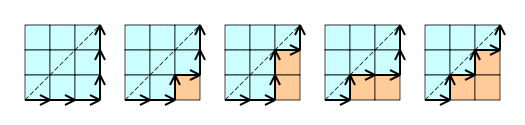
\includegraphics[width=0.4\paperwidth]{./img/catalan}
		\caption{\label{fig:catalan} Retículo de tamaño $\left(k,k\right)$.}
	\end{figure}
\end{example}

\begin{example}[La escalera]
	Un niño decide escalar una escalera con $n\geq 1$ de tal manera que cada paso que él despeja uno o dos de los pasos de la escalera %(vea)
	Encuentre la relación de recurrencia que sirva para calcular el número de diferentes maneras posibles de escalar la escalera.
\end{example}
Usamos la variable desconocida $x_{n}$ para denotar el número de maneras en las cuales el niño puede escalar la escalera de $n\geq1$ pasos. Es fácil de observar que $x_{1}=1$ y $x_{2}=2$ (dos pasos cada uno de longitud uno, o un paso de longitud dos escalones). Ahora sea $n\geq3$: si con el primer paso el niño mueve solo el primer escalón; existen claramente $x_{n-1}$ posibles maneras de escalar los que quedan. Si en cambio con el primer lugar, se suben dos peldaños de escalera.
%https://rajsain.files.wordpress.com/2013/11/randomized-algorithms-motwani-and-raghavan.pdf
%
%https://www.csie.ntu.edu.tw/~r97002/temp/Concrete%20Mathematics%202e.pdf
%
%https://link.springer.com/chapter/10.1007/978-3-642-61544-3_9
%
%https://link.springer.com/chapter/10.1007/978-94-011-1814-9_9
%
%https://link.springer.com/chapter/10.1007/978-3-319-15579-1_39
%
%https://link.springer.com/chapter/10.1007/978-94-011-2058-6_14
%
%https://link.springer.com/chapter/10.1007/BFb0120904
%
%https://link.springer.com/chapter/10.1007%2FBFb0120904
%
%https://link.springer.com/article/10.1007/BF00874886
%
%https://link.springer.com/search?date-facet-mode=between&showAll=true&query=recurrence+AND+relation&facet-discipline=%22Mathematics%22

%\motto{hola}
%\runinhead{xd}
%\subruninhead{xd}
%\begin{petit}
%A
%\end{petit}
\subsection{Problemas}

\begin{exercise}
Supongamos que $E_n$ es definido recursivamente en $\mathds{Z}^+$ por \[ E_0=0,E_1=2,\text{ y },E_{n+1}=2n\{E_n+E_{n-1}\} \text{ para }n\geq 1. \] Determine el valor de $E_{10}$.
\end{exercise}

\begin{solution}
	Suponga que $E_{n}$ es definida recursivamente sobre $P$ por \[ E_{0}=0,\quad E_{1}=2,\quad\text{y}\quad E_{n+1}=2n \LEFTRIGHT\{\}{E_{n}+E_{n-1}}\quad\forall n\geq1. \]
	El valor de $E_{10}$ se determina así:
	\begin{align*}
	E_{2}&=E_{1+1}=2(1)\LEFTRIGHT\{\}{E_{1}+E_{0}}=2\LEFTRIGHT\{\}{2+0}=4.\\
	E_{3}&=E_{2+1}=2(2)\LEFTRIGHT\{\}{E_{2}+E_{1}}=4\LEFTRIGHT\{\}{4+2}=24.\\
	E_{4}&=E_{3+1}=2(3)\LEFTRIGHT\{\}{E_{3}+E_{2}}=6\LEFTRIGHT\{\}{24+4}=168.\\
	E_{5}&=E_{4+1}=2(4)\LEFTRIGHT\{\}{E_{4}+E_{3}}=8\LEFTRIGHT\{\}{168+24}=1536.\\
	E_{6}&=E_{5+1}=2(5)\LEFTRIGHT\{\}{E_{5}+E_{4}}=10\LEFTRIGHT\{\}{1536+168}=17040.\\
	E_{7}&=E_{6+1}=2(6)\LEFTRIGHT\{\}{E_{6}+E_{5}}=12\LEFTRIGHT\{\}{17040+1536}=222912.\\
	E_{8}&=E_{7+1}=2(7)\LEFTRIGHT\{\}{E_{7}+E_{6}}=14\LEFTRIGHT\{\}{222912+17040}=3359328.\\
	E_{9}&=E_{8+1}=2(8)\LEFTRIGHT\{\}{E_{8}+E_{7}}=16\LEFTRIGHT\{\}{3359328+222912}=57315840.\\
	E_{10}&=E_{9+1}=2(9)\LEFTRIGHT\{\}{E_{9}+E_{8}}=18\LEFTRIGHT\{\}{57315840+3359328}=1092153024.
	\end{align*}
\end{solution}

%\begin{exercise}
%Supongamos que la función $f$ es definida recursivamente en $\mathds{Z}^+$ por \[ f(n)\coloneq \ccases{1 & \text{si }n=2^k\text{ para algún }k \in \mathds{N}.\\ f(n/2) & \text{si }n\text{ es par pero no una potencia de 2} \\ f(3n+1) & \text{si }n\text{ es impar.}}. \] Entonces
%	\begin{alignat*}{2}
%f(3)	=&f(10)	&&\qquad\text{ porque }3\text{ es impar}\\
%			=&f(5)	&&\qquad\text{ porque } 10=2\times 5\\
%			=&f(16)	&&\qquad\text{ porque }5\text{ es impar}\\
%			=&1&&\qquad\text{ porque } 16=2^4.
%\end{alignat*}
%\begin{enumerate}[(a)]
%	\item Mostrar que $f(11)$ también es igual a $1$.
%	\item Mostrar que $f(9)$, $f(14)$, y $f(25)$ son todos iguales a $f(11)$ y, por lo tanto, todos iguales a $1$.
%	\item Escriba un programa para hallar $f(27)$.
%\end{enumerate}
%?`Crees que esta función siempre dará el valor de $1$, sin importar con qué $n$ comiences? Busque la ``Conjetura de Collatz'' o el ``Problema del granizo''.
%\end{exercise}
%
%\begin{solution}
%	
%\end{solution}

%\begin{exercise}
%Podríamos definir una \emph{desajuste} como una $n$--permutación $S$ de $\left\{1,\ldots,n\right\}$ donde cada $S_{j}\neq j$ y luego definir $\bm{D_n}$ como el número de desajustes de $\left\{1,\ldots,n\right\}$. Entonces $D_{n}$ es la única sucesión que satisface la ecuación de recurrencia
%\begin{equation}\label{ex:1.3}
%D_{n}=\left(n-1\right)\left\{D_{n-1}+D_{n-2}\right\}\text{ para }n=3,4,5,\ldots
%\end{equation}
%con las condiciones iniciales $D_{1}=0$ y $D_{2}=1$.
%\begin{enumerate}[(a)]
%	\item Mostrar que $D_{2}=(2)\left(D_{1}\right)+(-1)^2$.
%	\item Use la inducción matemática para probar que para todo entero $n\geq2$, \[ D_{n}=(n)(D_{n-1})+{(-1)}^n. \]
%\end{enumerate}
%\end{exercise}
%
%\begin{solution}
%
%\end{solution}

%\begin{exercise}
%Use la inducción matemática y la ecuación \eqref{ex:1.3} para probar que \[ \forall n\in\mathds{Z}^{+}\colon\bm{D_n}=n!\sum_{j=0}^n\frac{(-1)^j}{j!}. \]
%\end{exercise}
%
%\begin{solution}
%	
%\end{solution}

%\begin{exercise}
%Supongamos que (o busque estos dos resultados de cálculo)
%\begin{enumerate}[A.]
%	\item $\forall x\in\mathds{R}\colon e^x=\sum_{j=0}^\infty\frac{x^j}{j!}$, entonces $e^{-1}=\sum_{j=0}^\infty\frac{(-1)^j}{j!},$
%	\item $\forall n\in\mathds{Z}^{+}\colon e^{-1}=\sum_{j=0}^n\frac{(-1)^j}{j!}+E_n$ donde $|E_n|<\left|\frac{(-1)^{n+1}}{(n+1)!}\right|=\frac{1}{(n+1)!}$.
%\end{enumerate}
%
%\begin{enumerate}[(a)]
%	\item Use el resultado de la pregunta anterior para mostrar \[ \frac{n!}{e}=D_{n}+n!E_{n}\quad\text{donde}\quad|n!E_n|<\frac{n!}{(n+1)!}=\frac{1}{n+1}\leq\frac{1}{2}. \]
%	\item Explique por qué $D_{n}-\frac{1}{2}\leq\frac{n!}{e}\leq D_{n}+\frac{1}{2}$.
%	\item ?`Es $\left\lceil\frac{n!}{e}\right\rceil=D_{n}$?
%\end{enumerate}
%
%\end{exercise}
%
%\begin{solution}
%	
%\end{solution}

%\begin{exercise}
%La \emph{función de Ackermann}\index{Ackermann!función} a veces es definida recursivamente en una forma ligeramente diferente
%\begin{enumerate}[label={Regla~\arabic*}]
%	\item $B\left(0,n\right)=n+1$ para $n=0,1,2,\ldots$,
%	\item $B\left(m,0\right)=B\left(m-1,1\right)$ para $m=1,2,3,\ldots$, y
%	\item $B\left(m,n\right)=B\left(m-1,B\left(m,n-1\right)\right)$ cuando ambos $m$ y $n$ son positivos.
%\end{enumerate}
%
%	\begin{enumerate}
%	\item Use inducción matemática para probar $\forall n\in\mathds{N}\colon B\left(1,n\right)=n+2$.
%	\item Use inducción matemática para probar $\forall n\in\mathds{N}\colon B\left(2,n\right)=3+2n$.
%	\item Use inducción matemática para probar $\forall n\in\mathds{N}\colon B\left(3,n\right)=2^{3+n}-3$.
%	\item Use inducción matemática para probar $\forall n\in\mathds{N}\colon B\left(4,n\right)=\left(2\uparrow\left[3+n\right]\right)-3$.
%	\item De una expresión usando el símbolo $\uparrow$ para los valores de $B\left(5,1\right)$ y $B\left(5,2\right)$.
%\end{enumerate}
%\end{exercise}
%
%\begin{solution}
%	
%\end{solution}

\begin{exercise}
Supongamos que $A$ es un conjunto de $2n$ objetos. Sea $P_{n}$ el número de diferentes maneras que los objetos en $A$ pueden ser ``emparejados'' (el número de diferentes particiones de $A$ en $2$--subconjuntos). Supongamos que $n\in\mathds{Z}^{+}$. Si $n=2$, entonces $A$ tiene cuatro elementos, $A=\left\{x_1,x_2,x_3,x_4\right\}$. Los tres posibles emparejamientos son:
\begin{enumerate}
	\item $x_{1}$ con $x_{2}$ y $x_{3}$ con $x_{4}$,
	\item $x_{2}$ con $x_{3}$ y $x_{2}$ con $x_{4}$,
	\item $x_{3}$ con $x_{4}$ y $x_{2}$ con $x_{3}$.
\end{enumerate}
Así $P_{2}=3$.

\begin{enumerate}[(a)]% TODO: Crear el programa en Python
	\item Mostrar que si $n=3$ y $A=\left\{x_{1},x_{2},x_{3},x_{4},x_{5},x_{6}\right\}$, existen $15$ posibles emparejamientos enumerándolos a todos:
	\begin{enumerate}
		\item $x_{1}$ con $x_{2}$ y $x_{3}$ con $x_{4}$ y $x_{5}$ con $x_{6}$.
		\item \ldots
	\end{enumerate}
	Así $\bm{P_3}=15$.
	\item Mostrar que $P_{n}$ debe satisfacer la RE $P_{n}=(2n-1)P_{n-1}$ para $\forall n\geq2$.
	\item Use esta ecuación de recurrencia y la inducción matemática para probar \[ P_{n}=\frac{(2n)!}{2^n\times n!}\quad\forall n\geq 1. \]
\end{enumerate}

\end{exercise}

\begin{solution}\leavevmode
	\begin{enumerate}[(a)]
		\item Los $15$ posibles emparejamientos son:
		\begin{enumerate}[1.]
			\item $x_{1}$ con $x_{2}$, $x_{3}$ con $x_{4}$ y $x_{5}$ con $x_{6}$.
			\item $x_{1}$ con $x_{2}$, $x_{3}$ con $x_{5}$ y $x_{4}$ con $x_{6}$.
			\item $x_{1}$ con $x_{2}$, $x_{3}$ con $x_{6}$ y $x_{4}$ con $x_{5}$.
			\item $x_{1}$ con $x_{3}$, $x_{2}$ con $x_{4}$ y $x_{5}$ con $x_{6}$.
			\item $x_{1}$ con $x_{3}$, $x_{2}$ con $x_{5}$ y $x_{4}$ con $x_{6}$.
			\item $x_{1}$ con $x_{2}$, $x_{2}$ con $x_{6}$ y $x_{4}$ con $x_{5}$.
			\item $x_{1}$ con $x_{4}$, $x_{2}$ con $x_{3}$ y $x_{5}$ con $x_{6}$.
			\item $x_{1}$ con $x_{4}$, $x_{2}$ con $x_{5}$ y $x_{3}$ con $x_{6}$.
			\item $x_{1}$ con $x_{4}$, $x_{2}$ con $x_{6}$ y $x_{3}$ con $x_{6}$.
			\item $x_{1}$ con $x_{5}$, $x_{2}$ con $x_{3}$ y $x_{4}$ con $x_{6}$.
			\item $x_{1}$ con $x_{5}$, $x_{2}$ con $x_{4}$ y $x_{3}$ con $x_{6}$.
			\item $x_{1}$ con $x_{5}$, $x_{2}$ con $x_{6}$ y $x_{3}$ con $x_{4}$.
			\item $x_{1}$ con $x_{6}$, $x_{2}$ con $x_{3}$ y $x_{4}$ con $x_{5}$.
			\item $x_{1}$ con $x_{5}$, $x_{2}$ con $x_{4}$ y $x_{3}$ con $x_{5}$.
			\item $x_{1}$ con $x_{6}$, $x_{2}$ con $x_{5}$ y $x_{3}$ con $x_{4}$.
		\end{enumerate}
		Así, $P_{3}=15$ posibles emparejamientos.
		\item Supongamos que $n\geq2$. Un elemento $x_{1}$ puede ser emparejado con cualquier de los $\left(2n-1\right)$ otros elementos en $A$. Esto resulta $2\left(n-2\right)=2\left(n-1\right)$ elementos aún por emparejar, y que pueden emparejarse en $P_{n-1}$ maneras. Así, el número de emparejamientos de $2n$ elementos es $P_{n}=\left(2n-1\right)\times P_{n-1}$.
		\item $P_{n}=(1)(3)\cdots\left(2n-1\right)$, esto es, el producto de los primeros $n$ naturales. Por inducción matemática:
		\begin{enumerate}[label={Paso~\arabic*}]
			\item $P_{1}=1$ que es el primer natural impar.
			\item Asuma que $\exists k\geq1$ donde $P_{k}=(1)(3)\cdots\left(2k-1\right)$.
			\item Si $n=k+1$, entonces para $n\geq2$ y
			\begin{align*}
			P_{k+1}&=\left(2\left[k+1\right]-1\right)P_{j}\quad\text{usando la RE}&\\
			&=\left(2k+1\right)\times(1)(3)\cdots\left(2k-1\right)\quad\text{del paso 2}&\\
			&=(1)(3)(5)\cdots\left(2k-1\right)\times\left(2\left[k+1\right]-1\right).
			\end{align*}
		\end{enumerate}
	\end{enumerate}
\end{solution}


\begin{exercise}
	Mostrar que $y_{n}=\frac{n(n-1)}{2}+c$ para $n>0$ es una solución de la relación de recurrencia \[ y_{n+1}=y_{n}+n. \]
\end{exercise}

\begin{solution}
	$z_{n+1}=\frac{\left[n+1\right]\left(\left[n+1\right]-1\right)}{2}+c=\frac{\left[n+1\right]\left(n\right)}{2}+c=\frac{n\left(n-1\right)+2n}{2}+c=z_{n}+n$.
\end{solution}

\begin{exercise}
Suponga que una sucesión es definida por: \[ f(0)=5\text{ y }f(n+1)=2\times f(n)+1\text{ para } n=0,1,2,\ldots. \]
\begin{enumerate}[(a)]
	\item Encuentre el valor de $f(10)$.
	\item Probar que la sucesión ni es una sucesión aritmética ni es una sucesión geométrica.
\end{enumerate}
\end{exercise}

\begin{solution}
	\begin{enumerate}
		\item
		\begin{align*}
		f(1)&=11, f(2)&=23, f(3)&=47, f(4)&=95, f(5)&=191,\\
		f(6)&=383, f(7)&=767, f(8)&=1535, f(9)&=3071, f(10)&=6143.
		\end{align*}
		\item $f(1)-f(0)=6$, pero $f(2)-f(1)=12$, así que $f$ no es un sucesión aritmética. Por otro lado, $\frac{f(1)}{f(0)}=\frac{11}{5}=\frac{121}{55}$. pero $\frac{f(2)}{f(1)}=\frac{23}{11}=\frac{115}{55}$, por lo tanto, $f$ no es una sucesión geométrica.
	\end{enumerate}
\end{solution}

%\begin{exercise}
%\begin{enumerate}[(a)]
%	\item Encuentre la solución general de la ecuación de recurrencia \[ S_{n}=3S_{n-1}-10\text{ para }n=1,2,\ldots \]\label{ex:1.10a}
%	\item Determine la solución particular donde $S_{0}=15$.
%	\item Use la fórmula en~\eqref{ex:1.10a} para evaluar $S_6$ y verifique su respuesta usando la ecuación de recurrencia en sí.
%\end{enumerate}
%\end{exercise}
%
%\begin{solution}
%	
%\end{solution}

%\begin{exercise}
%Suponga que $s_{0}=60$ y $s_{n+1}=(1/5)s_n-8$ para $n=0,1,\ldots$.
%\begin{enumerate}[(a)]
%	\item Encuentre $s_{1}$, $s_{2}$, y $s_{3}$.
%	\item Resuelva la relación de recurrencia para dar una fórmula para $s_{n}$.
%	\item ?`Es esa sucesión convergente? Si es así, ?`cuál es el límite?
%	\item ?`La serie correspondiente converge? Si es así, ?`cuál es el límite?
%\end{enumerate}
%\end{exercise}
%
%\begin{solution}
%	
%\end{solution}

%\begin{exercise}
%Suponga que $s_{0}=75$ y $s_{n+1}=(1/3)s_{n}-6$ para $n=0,1,\ldots$.
%\begin{enumerate}[(a)]
%	\item Encuentre $s_{1}$, $s_{2}$, y $s_{3}$.
%	\item Resuelva la relación de recurrencia para dar una fórmula para $s_{n}$.
%	\item ?`Es esa sucesión convergente? Si es así, ?`cuál es el límite?
%	\item ?`La serie correspondiente converge? Si es así, ?`cuál es límite?
%\end{enumerate}
%\end{exercise}
%
%\begin{solution}
%	
%\end{solution}

%\begin{exercise}
%\begin{enumerate}[(a)]
%	\item Mostrar que $f_{n}=A\times3^{n}+B\times2^{n}$ satisface la ecuación de recurrencia \[ f_{n}=5f_{n-1}-6f_{n-2}\text{ para }n\geq 2. \]
%	\item Encuentre la solución particular (valores para $A$ y $B$) para que \[ f_{0}=4\text{ y }f_{1}=17. \]
%\end{enumerate}
%
%\end{exercise}
%
%\begin{solution}
%	
%\end{solution}

\section{Recurrencias Lineales con coeficientes constantes}

Una relación de recurrencia lineal de orden $r$ con coeficientes constantes es una recurrencia del tipo:
\begin{align}\label{1}
c_{0}x_{n}+c_{1}x_{n-1}+\cdots+c_{r}x_{n-r}=h_{n},\forall n\geq r,
\end{align}
donde $c_{0},c_{1},\ldots,c_{r}$ son constantes reales o complejas, con $c_{0}$ y $c_{r}$ ambos diferentes de cero y $(h_{n})_{n\geq r}$ es una sucesión de números reales o complejos llamado sucesión de términos no homogéneos de la recurrencia. La recurrencia es llamada homogénea si la sucesión de términos no homogéneos es una sucesión nula, no homogénea si $h\neq0 $ para algún $n$. La relación de recurrencia:
\begin{align}\label{2}
c_{0}x_{n}+c_{1}x_{n-1}+\cdots+c_{r}x_{n-r}=0,\forall n\geq r,
\end{align}
es llamada la recurrencia homogénea asociada, o la parte homogénea de la recurrencia \eqref{1}. Como nosotros ya hemos notado, la recurrencia:
\begin{equation*}
c_{0}x_{n}+c_{1}x_{n-1}+\cdots+c_{r}x_{n-r}=h_{n},\forall n\geq r,
\end{equation*}
puede ser escrito equivalentemente como
\begin{equation*}
c_{0}x_{n+r}+c_{1}x_{n+(r-1)}+\cdots+c_{r}x_{n}=h_{n+r},\forall n\geq 0.
\end{equation*}
Se puede utilizar cualquiera de las formas presentadas.

\begin{remark}
	Cada $r$-secuencia de valores asignados a las $r$ incógnitas desconocidas de la relación de recurrencia
	\begin{equation*}
	c_{0}x_{n}+c_{1}x_{n-1}+\cdots+c_{r}x_{n-r}=h_{n},\forall n\geq r,
	\end{equation*}
	determina de forma única una solución. Al resolver una relación de recurrencia lineal, el siguiente principio es fundamental importancia.
\end{remark}

\begin{proposition}[Principio de superposición]\index{Principio de superposición}
	Sean ${(u_{n})}_{n}$, ${(V_{n})}_{n}$ respectivamente las soluciones de las relaciones de recurrencia lineal.
	\begin{align*}
	c_{0}x_{n}+c_{1}x_{n-1}+\cdots+c_{r}x_{n-r}&=h_{n},\quad n\geq r
	\intertext{y}
	c_{0}x_{n}+c_{1}x_{n-1}+\cdots+c_{r}x_{n-r}&=k_{n},\quad n\geq r,
	\end{align*}
	con partes homogéneas iguales y secuencias de términos no homogéneos $(h_{n})_{n}$ y $(k_{n})_{n}$. Para cualquier par de constantes $A$ y $B$, la sucesión $(Av_{n}+Bv_{n})_{n}$ es una solución de la relación de recurrencia. \[ c_{0}x_{n}+c_{1}x_{n-1}+\cdots+c_{r}x_{n-r}=Ah_{n}+Bk_{n}. \] La solución general de la relación de recurrencia
	\begin{equation}\label{eq:super}
	c_{0}x_{n}+c_{1}x_{n-1}+\cdots+c_{r}x_{n-r}=h_{n},\quad n\geq r.
	\end{equation}
\end{proposition}

\begin{proof}\leavevmode
	\begin{enumerate}
		\item Uno tiene fácilmente
		\begin{equation*}
		\begin{split}
		&c_{0}(Au_{n}+Bv_{n})+c_{1}(Au_{n-1}+Bv_{n-1})+\cdots+c_{r}(Au_{n-r}+Bv_{n-r})=\\
		&\phantom{c_{0}(Au_n+}=A(c_{0}u_{n}+c_{1}u_{n-1}+\cdots+c_{r}u_{n-r})+B(c_{0}v_{n}+c_{1}v_{n-i}+\cdots+c_{r}v_{n-r})\\
		&\phantom{c_{0}(Au_n+}=Ah_{n}+Bk_{n}.
		\end{split}
		\end{equation*}
		\item Sea $(u_{n})_{n}$ una solución particular de \eqref{eq:super}. Por el punto previo nosotros conocemos que $(v_{n})_{n}=(u_{n})_{n}+(v_{n}-u_{n})_{n}$ es una solución de \eqref{eq:super} si y solo si $v_{n}-u_{n}$ es una solución de la recurrencia homogénea asociada. Por lo tanto cada solución de \eqref{eq:super} es obtenida añadiendo una solución de la  recurrencia homogénea asociada para $(u_{n})_{n}$.
	\end{enumerate}
\end{proof}

\section{Relación de recurrencia lineal con homogénea con coeficientes constantes}

La sucesión nula es una solución de cualquier relación de recurrencia lineal. La estructura de la solución general de una relación de recurrencia lineal homogénea corresponde a la estructura de la solución general de un sistema de ecuaciones lineales homogéneas.
\begin{proposition}[Teorema principal]
	Considere la relación de recurrencia lineal homogénea de orden $r$:
	\begin{equation}\label{eq:homo}
	c_{0}x_{n}+c_{1}x_{n-1}+\cdots+c_{r}x_{n-r}=0,\quad n\geq r\quad\left(c_{0}c_{r}\neq0\right)
	\end{equation}
	\begin{enumerate}
		\item Cualquier combinación lineal de soluciones de \eqref{eq:homo} es de nuevo una solución de \eqref{eq:homo}.
		\item Existe $r$ soluciones de \eqref{eq:homo} tal que cualquier otra solución de \eqref{eq:homo} puede ser expresado únicamente como su combinación lineal.
	\end{enumerate}
\end{proposition}

\begin{proof}\leavevmode
	\begin{enumerate}
		\item Esto sigue inmediatamente por el ``Principio de Superposición''.
		\item Para todo $i\in\left\{0,\ldots,r-1 \right\}$ sea $\left(u^{i}_{n}\right)_{n}$ la solución de \eqref{eq:homo} con $r$--sucesión de valores iniciales iguales a $0$ para índices $j\neq i$, iguales a $1$ en índices $i$, es decir: \[ u^{i}_{j}=0\text{ si }j\neq i,\quad u^{i}_{i}=1\quad j\in\left\{0,\ldots,r-1 \right\}. \]
		Consideramos ahora alguna solución $(a_{n})_{n}$ de \eqref{eq:homo}; la combinación lineal \[ a_{0}{\left(u^{0}_{n}\right)}_{n}+a_{1}{\left(u^{1}_{n}\right)}_{n}+\cdots+a_{r-1}(u^{r-1}_{n})_{n}, \]	es una solución de \eqref{eq:homo} con secuencia de datos iniciales $\left(a_{0},\ldots,a_{r-1}\right)$. Ya que la sucesión de valores iniciales determinan la solución de una relación de recurrencia, uno tiene \[ {\left(a_{n}\right)}_{n}=a_{0}\left(u^{0}_{n}\right)_{n}+a_{1}\left(u^{1}_{n}\right)_{n}+\cdots+a_{r-1}\left(u^{r-1}_{n}\right)_{n}. \]
	\end{enumerate}
\end{proof}

\begin{definition}[Polinomio característico]\index{Relación de recurrencia!polinomio característico}
	Definimos el \emph{polinomio característico} de una relación de recurrencia con coeficientes constantes de orden $r$ de la siguiente manera: \[ c_{0}x_{n}+c_{1}x_{n-1}+\cdots+c_{r}x_{n-r}=h_{n},\quad n\geq r\left(c_{0}c_{r}\neq0\right), \] para el polinomio de grado $r$: \[ P(X)\coloneqq c_{0}X^{r}+c_{1}X^{r-1}+\cdots+c_{r}. \] Cada polinomio de grado $r$ tiene exactamente $r$ raíces complejas contando con su multiplicidad. Vemos ahora que la sucesión de las potencias naturales de una determinada raíz del polinomio característico de una relación de recurrencia lineal es una solución de la correspondiente relación homogénea.
\end{definition}

\begin{proposition}[Raíz del polinomio característico]\index{Relación de recurrencia!polinomio característico!raíz}
	Sea $\lambda\in\mathds{C}$. La sucesión $\left(\lambda^{n}\right)_{n}$ de las potencias de $\lambda$ es una solución de la relación de recurrencia lineal homogénea
	\begin{align}\label{5}
	c_{0}x_{n}+c_{1}x_{n-1}+\cdots+c_{r}x_{n-r}=0,\quad n\leq r \quad (c_{0}c_{r}\neq 0),
	\end{align}
	sii $\lambda$ es una raíz de este polinomio característico.
\end{proposition}

\begin{proof}
	Dado que $c_{r}\neq0$, las raíces del polinomio característico deben ser necesariamente no nulas. Sustituyendo los valores de la sucesión ${\left(\lambda^{n}\right)}_{n}$ en la recurrencia, uno tiene \[ c_{0}x_{n}+c_{1}x_{n-1}+\cdots+c_{r}x_{n-r}=0, \] y dividiendo por $\lambda^{n-r}\neq0$ \[ c_{0}\lambda^{r}+c_{1}\lambda^{r-1}+\cdots+c_{r}=0. \]	Por lo tanto, la sucesión ${\left(\lambda^{n}\right)}_{n}$ es una solución de \eqref{5} sii $\lambda$ es una raíz del polinomio $c_{0}X^{r}+c_{1}X^{r-1}+\cdots+c_{r}$.
\end{proof}

En general, no es fácil encontrar las raíces de un polinomio de grado mayor que dos, aunque uno puede siempre usar un adecuado CAS. El siguiente criterio simple, sin embargo, muestra cómo encontrar las raíces racionales de un polinomio con coeficientes enteros.

\begin{proposition}[Las raíces racionales de un polinomio con coeficientes enteros]
	Sea $P(X)=c_{0}X^{r}+c_{1}X^{r-1}+\cdots+c_{r}$ un polinomio con coeficientes enteros $c_{0}\ldots c_{r}\in\mathds{Z}$, con $c_{0}\neq 0$. Si la fracción $\tfrac{a}{b}$ con $a,b\in\mathds{Z}$ con $\operatorname{mcd}=1$ es una raíz de $P(X)$, luego $a\divides c_{r}$ y $b\divides c_{0}$. En particular, si $c_{0}=\pm1$ las raíces racionales del polinomio $P(X)$ son enteros que dividen a $c_{r}$.
\end{proposition}

\begin{proof}
	Dado $c_{0}\left(\frac{a}{b}\right)^{r}+c_{1}{\left(\frac{a}{b}\right)}^{r-1}+\cdots+c_{r-1}\left(\frac{a}{b}\right)+c_{r}=0$, multiplicado por $b^{r}$ obtenemos: \[ 	c_{0}a^{r}+c_{1}a^{r-1}b+\cdots+c_{r-1}ab^{r-1}+c_{r}b^{r}=0. \] Como $a\divides c_{0}a^{r}+c_{1}a^{r-1}b+\cdots+c_{r-1}ab^{r-1}$, luego tiene que dividir también $c_{r}b^{r}$, y por lo tanto, al no tener $a$ y $b$ factores comunes, $a\divides c_{r}$. Análogamente $b\divides c_{0}a^{r}$ y por lo tanto divide a $c_{0}$.
\end{proof}

\begin{example}[Polinomio característico]
	La recurrencia homogénea de segundo orden: \[ x_{n}=2x_{n-1}-2x_{n-2},\quad n\geq2, \] tiene polinomio característico $X^{2}-2X+2$ cuyas raíces son $\lambda_{1}=1-i$ y $\lambda_{2}=1+i$. Las sucesiones ${\left((1-i)^{n}\right)}_{n}$ y ${\left((1+i)^{n}\right)}_{n} $ son las soluciones bases de la recurrencia. La solución general compleja de la recurrencia es: \[ x_{n}=A_{1}{\left(1-i\right)}^{n}+A_{2}{\left(1+i\right)}^{n},\quad n\geq 0, \] con la variante de $A_{1}$ y $A_{2}$ entre los números complejos. Veamos la solución real general. Uno tiene: \[ \lambda_{1}=1-i=\sqrt{2}\left(\frac{\sqrt{2}}{2}-\frac{\sqrt{2}}{2}i\right)=\sqrt{2}\left(\cos\left(\frac{\pi}{4}\right)-i\sen\left(\frac{\pi}{4}\right)\right) \] y \[ \lambda_{2}=1+i=\overline{\lambda_{1}}=\sqrt{2}\left(\cos\left(\frac{\pi}{4}\right)-i\sen\left(\frac{\pi}{4}\right)\right). \] Luego, las sucesiones ${\left(2^{n/2}\cos\left( \frac{n\pi}{4}\right)\right)}_{n}$ y ${\left(2^{n/2}\sen\left(\frac{n\pi}{4}\right)\right)}_{n}$ son las soluciones base reales de la recurrencia. Por lo tanto, la solución general real de la recurrencia es: \[ x_{n}=A_{1}2^{n/2}\cos\left(\frac{n\pi}{4}\right)+A_{2}2^{n/2}\sen\left(\frac{n\pi}{4}\right),\quad n\geq 0, \] con la variación de $A_{1}$ y $A_{2}$ entre los números reales.
\end{example}

%\begin{claim}
%Afirmo que el Lema de Zorn es cierto.
%\end{claim}
%
%\begin{proof}
%$\smartqed$
%
%$\qed$
%\end{proof}
%
%\begin{case}
%	
%\end{case}
%
%\begin{conjecture}
%	
%\end{conjecture}
%
%\begin{corollary}
%	
%\end{corollary}
%
%\begin{definition}
%	
%\end{definition}
%
%\begin{example}[Quispe]
%	
%\end{example}
%
%\begin{lemma}
%	
%\end{lemma}
%
%\begin{note}
%	
%\end{note}
%
%\begin{problem}
%	
%\end{problem}
%
%\begin{property}
%	
%\end{property}
%
%\begin{proposition}
%	
%\end{proposition}
%
%\begin{question}{Bryan}
%	
%\end{question}
%
%\begin{remark}
%
%\end{remark}
%
%\begin{theorem}
%
%\end{theorem}
%
%\begin{trailer}{Enfatizar párrafos}
%\end{trailer}
%
%\begin{question}{?`Qué hora es?}
%\end{question}
%
%\begin{important}{Importante}
%	A
%\end{important}
%
%\begin{warning}{Atención}
%	
%\end{warning}
%
%\begin{tips}{Consejos}
%	
%\end{tips}
%
%\begin{overview}{Enfatizar párrafos completos}
%	
%\end{overview}
%
%\begin{backgroundinformation}{Información de fondo}
%	
%\end{backgroundinformation}
%
%\begin{legaltext}{Texto legal}
%	
%\end{legaltext}
\subsection{Relación de recurrencia}

\subsubsection{Con coeficientes constantes}

\subsubsection{Homogénea}
\section{Ecuación en diferencias}\label{sec:difference}\index{Ecuación en diferencias!definición}

Aquí es conveniente representar cualquier sucesión de números reales $(a_{n})_{n} $ como la función $f\colon\mathds{N}\rightarrow\mathds{R}$ definido por: \[ f(n)=a_{n},\quad\forall n\in\mathds{N}. \] Dadas dos funciones $f,g\colon\mathds{N}\rightarrow\mathds{R}$ y $r\in\mathds{R} $ consideremos las funciones: \[ (f+g)(n)=f(n)+g(n),\quad\text{y}\quad(rf)(n)=rf(n)\quad\forall n\in\mathds{N}. \] Dotado de estas operaciones, el conjunto de funciones de $\mathds{N}\rightarrow\mathds{R}$ es un $\mathds{R}$--espacio vectorial de funciones. También consideraremos la función: \[ (fg)(n)=f(n)g(n)\forall k\in\mathbb{N}. \] Un mapa lineal del espacio de funciones de $\mathds{N}$ a $ \mathds{R}$ en sí mismo es un operador.

\begin{definition}[Operador identidad y operador de cambio]
Consideramos el espacio de funciones de $\mathds{N}\to\mathds{R}$. Para cada función $f\colon\mathds{N}\rightarrow\mathds{R}$ el operador identidad y el operador de cambio $\theta$ están definidos: \[ \mathds{I}(f)=f\quad\text{y}\quad\theta(f)(n)=f(n+1)\quad\forall n\in\mathds{N}. \] Uno verifica inmediatamente que la identidad y el operador de cambio son de hecho lineales.
\end{definition}

\begin{proposition}[Linealidad de la identidad y el operador de cambio]
Sean las funciones $f,g\colon\mathds{N}\to\mathds{N}$ y $c\in\mathds{R}$. Luego tenemos:
\begin{enumerate}
	\item $\mathds{I}\left(f+g\right)(n)=\mathds{I}(f)(n)+\mathds{I}(g)(n)$.
	\item $\mathds{I}\left(cf\right)(n)=c\mathds{I}(f)(n)$ y $\theta\left(cf\right)(n)=c\theta(f)(n)$.
\end{enumerate}
\end{proposition}

\begin{proof}
	Sea $n\in\mathds{N}$, luego:
	\begin{align*}
	\theta(f+g)(n)&=(f+g)(n+1)=f(n+1)+g(n+1)=\theta(f)(n)+\theta(g)(n).\\
	\theta(cf)(n)&=(cf)(n+1)=cf(n+1)=c\theta(f)(n).
	\end{align*}
	Se verifica la linealidad de $\mathds{I}$ inmediatamente.
\end{proof}

Para cualquier operador $T$, será conveniente un ligero abuso de notación, para escribir $Tf(n)$ en lugar de $T(f)(n)$. Además en algunos casos, por ejemplo cuando $f$ depende de otros parámetros, uno escribe $T_{n}f(n)$ en lugar de $Tf(n)$ para evitar la ambigüedad. Así, por ejemplo, denotada por $\mathds{I}_{\mathds{N}}\colon\mathds{N}\rightarrow\mathds{N}$ la función definida por $\mathds{I}_{\mathds{N}}(n)=n$ para cada $n\in\mathds{N} $ escribiremos $\theta n=n+1$ en lugar de $\theta(\mathds{I}_{\mathds{N}})(n)=n+1$. Análogamente $\theta n^{2}=(n+1)^{2}$, $\theta_{n}n^{a}=(n+1)^{a}$ y $\theta_{n}a^{n}=a^{n+1}$ para cada $a\in\mathds{R}$.

Para las funciones de valor real de una variable de número natural ahora introducimos el análogo de la derivada habitual para funciones de valor real de una variable real:

\begin{definition}[Operador de cambio]
	El operador diferencia es el operador $\bigtriangleup$ que a cada función $f\colon\mathds{N}\rightarrow\mathds{R}$ asigna la función $\bigtriangleup f\colon\mathds{N}\rightarrow \mathds{R}$, definido de la siguiente manera: \[ \bigtriangleup f(n)=f(n+1)-f(n),\quad\forall n\in\mathds{N}. \]
\end{definition}

\begin{remark}
	Usando el operador de cambio, uno tiene $\bigtriangleup=\theta-\mathds{I}$, es decir: \[ \bigtriangleup f=\theta f-f,\quad\forall f\colon\mathds{N}\rightarrow\mathds{R}. \] Claramente, para cada función $f\colon\mathds{N}\rightarrow\mathds{R}$, uno tiene: \[ \bigtriangleup f(k)=\frac{f(k+1)-f(k)}{1}, \] entonces $\bigtriangleup f\colon\mathds{N}\rightarrow\mathds{R}$ es una función que mide el cociente de diferencia de $f$ sobre el intervalo más pequeño posible de números naturales, es decir, un intervalo de longitud uno. En este sentido, el operador diferencia constituye el análogo discreto de la noción de derivada para funciones de una variable real. En lo que sigue, el lector tendrá ocasión para anotar analogías y contrastes entre estas dos nociones.
\end{remark}

Al igual que la derivada, el operador de diferencia es lineal: de hecho, es una diferencia de dos operadores lineales.

\begin{proposition}[Linealidad de la diferencia]
	Sean $ f,g\colon\mathds{N}\rightarrow\mathds{R}$ y $c\in\mathds{R}$. Luego uno tiene:
	\begin{enumerate}
		\item $\bigtriangleup\left(f+g\right)=\bigtriangleup f+\bigtriangleup g$.
		\item $\bigtriangleup(cf)=c\bigtriangleup f$.
	\end{enumerate}
\end{proposition}


\begin{proof}
	Como $ \bigtriangleup=\theta-\mathds{I}$ se obtiene:
	\begin{enumerate}
		\item $\bigtriangleup\left(f+g\right)=\left(\theta-\mathds{I}\right)\left(f+g\right)=\theta\left(f+g\right)-\mathds{I}\left(f+g\right)=\theta(f)-f+\theta(g)-g=\bigtriangleup(f)-\bigtriangleup(g)$.
		\item $\bigtriangleup\left(cf\right)=\left(\theta-\mathds{I}\right)\left(cf\right)=\theta\left(cf\right)-\mathds{I}\left(cf\right)=c\theta(f)-cf=c(\theta-\mathds{I})(f)=c\bigtriangleup(f)$.
	\end{enumerate}
\end{proof}
Ahora vemos cómo el operador de diferencia actúa en algunas funciones simples con dominio $\mathds{N}$.

\begin{example}\leavevmode
	\begin{enumerate}
		\item Funciones constantes: al igual que en el caso de la derivada de una  constante. Funciona con dominios en $\mathds{R}$, aquí también tenemos que la diferencia de una función constante (con dominio $\mathds{N}$) es igual a la función cero: de hecho, si $f(n)=c\in\mathds{R}$ por cada $n\in\mathds{N}$, entonces \[ \bigtriangleup f(k)=f(k+1)-f(k)=c-c=0. \]
		\item Función de identidad en los números naturales: al igual que en el caso continuo, la diferencia de la función de identidad $I_{\mathds{N}}\colon\mathds{N}\rightarrow \mathds{N}$ es la función constante $n=1$ para todo $n\in\mathds{N}$. De hecho, \[ \bigtriangleup I_{\mathds{N}}(n)=I_{\mathds{N}}(n+1)-1=n+1-n=1. \]
		\end{enumerate}
\end{example}

\begin{example}
	Los operadores de cambio y diferencia conmutan. Más explícitamente, uno tiene \[ \bigtriangleup\circ\theta=\theta\circ\bigtriangleup. \]
\end{example}

\begin{proof}
De hecho, para cada $n\in\mathds{N} $ y cada función $f\colon\mathds{N}\rightarrow\mathds{R}$ uno tiene
	\begin{align*}
		\bigtriangleup\left(\theta f\right)(n)&=\theta f\left(n+1\right)-\theta f(n)=f(n+2)-f\left(n+1\right),\\
		\shortintertext{mientras}
		\theta\left(\bigtriangleup f\right)(n)&=\bigtriangleup f\left(n+1\right)=f(n+2)-f(n+1).
	\end{align*}
Por lo tanto, uno tiene $\bigtriangleup\left(\theta f\right)=\theta\left(\bigtriangleup f\right)(n)$.
\end{proof}
La fórmula para la diferencia de un producto se parece a la del derivado de un producto, excepto la introducción del operador de turno:
\begin{proposition}[Diferencia de un producto]
Si $f,g\colon\mathds{N}\rightarrow\mathds{R}$, luego \[ \bigtriangleup\left(fg\right)=\bigtriangleup f\theta g+f\bigtriangleup g. \]
\end{proposition}

\begin{remark}
	Cabe destacar el hecho evidente de que a pesar de la aparente falta de simetría, uno tiene $\bigtriangleup\left(fg\right)=\bigtriangleup\left(gf\right)$.
\end{remark}

\begin{proof}
	\begin{align*}
		\bigtriangleup\left(f(n)g(n)\right)
		&=f\left(n+1\right)g\left(n+1\right)-f(n)g(n)\\
		&=f(n+1)g(n+1)-f(n)g(n+1)+f(n)(n+1)-f(n)g(n)\\
		&=(f(n+1)-f(n))g(n+1)+f(n)g(n+1)-g(n)\\
		&=\bigtriangleup f(n)\theta g(n)+f(n)\bigtriangleup g(n).
	\end{align*}
\end{proof}

\

Una ecuación en diferencias es una expresión de la forma: \[ G\left(n,f(n),f(n+1),\ldots,f(n+k)\right)=0,\forall n\in\mathds{Z} \] donde $f$ es una función definida en $\mathds{Z}$.

Si después de simplificar esta expresión quedan los términos $f\left(n+k_{1}\right)$ y $f\left(n+k_{2}\right)$ como el mayor y el menor, respectivamente. Se dice que la ecuación es de orden $k=k_{1}-k_{2}$.

\begin{example}[Ecuación en diferencias de orden $3$]
	La ecuación dada por \[ 5f(n+4)-4f(n+2)+f(n+1)+(n-2)^{3}=0 \] es de orden $4-1=3$.
\end{example}

Una ecuación en diferencias de orden $k$ se dice que es \emph{lineal}\index{Ecuación en diferencias!lineal} si puede expresarse de la forma: \[ p_{0}(n)f(n+k)+p_{1}(n)f(0+k-1)+\cdots+p_{k}(n)f(n)=g(n), \] donde los coeficientes $p_{i}$ son funciones definidas en $\mathds{Z}$.

El caso más sencillo es cuando los coeficientes son constantes $p_{i}(n)=a_{i}$: \[ a_{0}f(n+k)+a_{1}f(n+k-1)+\cdots+a_{k}f(n)=g(n). \] La ecuación en diferencias se dice que es \emph{homogénea}\index{Ecuación en diferencias!homogénea} en el caso que $g(n)=0$, y completa en el caso contrario.

\begin{theorem}{}
	Dada la ecuación en diferencias lineal de coeficientes constantes y de orden $ K $: \[ a_{0}f(n+k)+a_{1}f(n+k-1)+\cdots+a_{k}f(n)=g(n) \] el problema de hallar una función definida $\mathds{Z}$, que verifique la ecuación, y tales que en los $k$ enteros consecutivos $n_{0},n_{0}+1,\ldots,n_{0}+k-1$ tome los valores dados $c_{0},c_{1},\ldots,c_{k-1}$, tiene solución única.
\end{theorem}

\begin{theorem}{}
	Dada una ecuación en diferencias lineal homogénea de coeficientes constantes y de orden $k$. Si una solución $f$ es nula en $k$ enteros consecutivos, entonces $f$ es idénticamente nula.
\end{theorem}

\begin{theorem}{}
	Toda combinación lineal de soluciones de una ecuación en diferencias lineal homogénea de coeficientes constantes y de orden $k$ es también solución de dicha ecuación.
\end{theorem}

\begin{definition}[Solución de una ecuación en diferencias homogénea]
Sea la ecuación en diferencias lineal homogénea de coeficientes constantes y de orden $k$. \[ a_{0}f(n+k)+a_{1}f(n+k-1)+\cdots+a_{k}f(n)=0,\quad\forall k\in\mathds{Z}. \] Buscaremos soluciones del tipo $f(n)=r^{n}.$ Entonces, \[ r^{n}\left(a_{0}r^{k}+a_{1}r^{k-1}+\cdots+a_{k}\right)=0\implies r^{n}(a_{0}r^{k}+a_{1}r^{k-1}+\cdots+a_{k})=0. \] Por tanto, $r$ es raíz de la \textbf{ecuación característica} \[ (a_{0}r^{k}+a_{1}r^{k-1}+\cdots+a_{k})=0. \]
\end{definition}

El estudio de la solución dependería de si las raíces de la ecuación característica son simples o múltiples.
\begin{example}
	Hallar la solución de \[ f(n+2)-4f(n+1)+3f(n)=0\quad\forall n\in\mathds{Z},\quad f(0)=0,\quad f(1)=1. \] La ecuación característica es \[ r^{2}-4r+3=0\rightarrow r_{1}=3,\quad r_{2}=1. \] Por lo tanto: \[ f(n)=c_{1}3^{n}+c_{2}1^{n}=c_{1}3^{n}+c_{2}. \] Por otra parte:
	\begin{equation*}
	\left.\begin{aligned}
	f(0)&=\phantom{1}c_{1}+c_{2}=0\\
	f(1)&=3c_{1}+c_{2}=1
	\end{aligned}
	\right\}
	\longrightarrow c_{1}=\frac{1}{2},\quad c_{2}=-\frac{1}{2}.
	\end{equation*}
De donde \[ f(n)=\frac{1}{2}\cdot3^{n}-\frac{1}{2}=\frac{3^{n}-1}{2}. \]
\end{example}
\section{Recurrencias Lineales con coeficientes constantes}

Una relación de recurrencia lineal de orden $r$ con coeficientes constantes es una recurrencia del tipo:
\begin{align}\label{1}
c_{0}x_{n}+c_{1}x_{n-1}+\cdots+c_{r}x_{n-r}=h_{n},\forall n\geq r,
\end{align}
donde $c_{0},c_{1},\ldots,c_{r}$ son constantes reales o complejas, con $c_{0}$ y $c_{r}$ ambos diferentes de cero y $(h_{n})_{n\geq r}$ es una sucesión de números reales o complejos llamado sucesión de términos no homogéneos de la recurrencia. La recurrencia es llamada homogénea si la sucesión de términos no homogéneos es una sucesión nula, no homogénea si $h\neq0 $ para algún $n$. La relación de recurrencia:
\begin{align}\label{2}
c_{0}x_{n}+c_{1}x_{n-1}+\cdots+c_{r}x_{n-r}=0,\forall n\geq r,
\end{align}
es llamada la recurrencia homogénea asociada, o la parte homogénea de la recurrencia \eqref{1}. Como nosotros ya hemos notado, la recurrencia:
\begin{equation*}
c_{0}x_{n}+c_{1}x_{n-1}+\cdots+c_{r}x_{n-r}=h_{n},\forall n\geq r,
\end{equation*}
puede ser escrito equivalentemente como
\begin{equation*}
c_{0}x_{n+r}+c_{1}x_{n+(r-1)}+\cdots+c_{r}x_{n}=h_{n+r},\forall n\geq 0.
\end{equation*}
Se puede utilizar cualquiera de las formas presentadas.

\begin{remark}
	Cada $r$-secuencia de valores asignados a las $r$ incógnitas desconocidas de la relación de recurrencia
	\begin{equation*}
	c_{0}x_{n}+c_{1}x_{n-1}+\cdots+c_{r}x_{n-r}=h_{n},\forall n\geq r,
	\end{equation*}
	determina de forma única una solución. Al resolver una relación de recurrencia lineal, el siguiente principio es fundamental importancia.
\end{remark}

\begin{proposition}[Principio de superposición]\index{Principio de superposición}
	Sean ${(u_{n})}_{n}$, ${(V_{n})}_{n}$ respectivamente las soluciones de las relaciones de recurrencia lineal.
	\begin{align*}
	c_{0}x_{n}+c_{1}x_{n-1}+\cdots+c_{r}x_{n-r}&=h_{n},\quad n\geq r
	\intertext{y}
	c_{0}x_{n}+c_{1}x_{n-1}+\cdots+c_{r}x_{n-r}&=k_{n},\quad n\geq r,
	\end{align*}
	con partes homogéneas iguales y secuencias de términos no homogéneos $(h_{n})_{n}$ y $(k_{n})_{n}$. Para cualquier par de constantes $A$ y $B$, la sucesión $(Av_{n}+Bv_{n})_{n}$ es una solución de la relación de recurrencia. \[ c_{0}x_{n}+c_{1}x_{n-1}+\cdots+c_{r}x_{n-r}=Ah_{n}+Bk_{n}. \] La solución general de la relación de recurrencia
	\begin{equation}\label{eq:super}
	c_{0}x_{n}+c_{1}x_{n-1}+\cdots+c_{r}x_{n-r}=h_{n},\quad n\geq r.
	\end{equation}
\end{proposition}

\begin{proof}\leavevmode
	\begin{enumerate}
		\item Uno tiene fácilmente
		\begin{equation*}
		\begin{split}
		&c_{0}(Au_{n}+Bv_{n})+c_{1}(Au_{n-1}+Bv_{n-1})+\cdots+c_{r}(Au_{n-r}+Bv_{n-r})=\\
		&\phantom{c_{0}(Au_n+}=A(c_{0}u_{n}+c_{1}u_{n-1}+\cdots+c_{r}u_{n-r})+B(c_{0}v_{n}+c_{1}v_{n-i}+\cdots+c_{r}v_{n-r})\\
		&\phantom{c_{0}(Au_n+}=Ah_{n}+Bk_{n}.
		\end{split}
		\end{equation*}
		\item Sea $(u_{n})_{n}$ una solución particular de \eqref{eq:super}. Por el punto previo nosotros conocemos que $(v_{n})_{n}=(u_{n})_{n}+(v_{n}-u_{n})_{n}$ es una solución de \eqref{eq:super} si y solo si $v_{n}-u_{n}$ es una solución de la recurrencia homogénea asociada. Por lo tanto cada solución de \eqref{eq:super} es obtenida añadiendo una solución de la  recurrencia homogénea asociada para $(u_{n})_{n}$.
	\end{enumerate}
\end{proof}

\section{Relación de recurrencia lineal con homogénea con coeficientes constantes}

La sucesión nula es una solución de cualquier relación de recurrencia lineal. La estructura de la solución general de una relación de recurrencia lineal homogénea corresponde a la estructura de la solución general de un sistema de ecuaciones lineales homogéneas.
\begin{proposition}[Teorema principal]
	Considere la relación de recurrencia lineal homogénea de orden $r$:
	\begin{equation}\label{eq:homo}
	c_{0}x_{n}+c_{1}x_{n-1}+\cdots+c_{r}x_{n-r}=0,\quad n\geq r\quad\left(c_{0}c_{r}\neq0\right)
	\end{equation}
	\begin{enumerate}
		\item Cualquier combinación lineal de soluciones de \eqref{eq:homo} es de nuevo una solución de \eqref{eq:homo}.
		\item Existe $r$ soluciones de \eqref{eq:homo} tal que cualquier otra solución de \eqref{eq:homo} puede ser expresado únicamente como su combinación lineal.
	\end{enumerate}
\end{proposition}

\begin{proof}\leavevmode
	\begin{enumerate}
		\item Esto sigue inmediatamente por el ``Principio de Superposición''.
		\item Para todo $i\in\left\{0,\ldots,r-1 \right\}$ sea $\left(u^{i}_{n}\right)_{n}$ la solución de \eqref{eq:homo} con $r$--sucesión de valores iniciales iguales a $0$ para índices $j\neq i$, iguales a $1$ en índices $i$, es decir: \[ u^{i}_{j}=0\text{ si }j\neq i,\quad u^{i}_{i}=1\quad j\in\left\{0,\ldots,r-1 \right\}. \]
		Consideramos ahora alguna solución $(a_{n})_{n}$ de \eqref{eq:homo}; la combinación lineal \[ a_{0}{\left(u^{0}_{n}\right)}_{n}+a_{1}{\left(u^{1}_{n}\right)}_{n}+\cdots+a_{r-1}(u^{r-1}_{n})_{n}, \]	es una solución de \eqref{eq:homo} con secuencia de datos iniciales $\left(a_{0},\ldots,a_{r-1}\right)$. Ya que la sucesión de valores iniciales determinan la solución de una relación de recurrencia, uno tiene \[ {\left(a_{n}\right)}_{n}=a_{0}\left(u^{0}_{n}\right)_{n}+a_{1}\left(u^{1}_{n}\right)_{n}+\cdots+a_{r-1}\left(u^{r-1}_{n}\right)_{n}. \]
	\end{enumerate}
\end{proof}

\begin{definition}[Polinomio característico]\index{Relación de recurrencia!polinomio característico}
	Definimos el \emph{polinomio característico} de una relación de recurrencia con coeficientes constantes de orden $r$ de la siguiente manera: \[ c_{0}x_{n}+c_{1}x_{n-1}+\cdots+c_{r}x_{n-r}=h_{n},\quad n\geq r\left(c_{0}c_{r}\neq0\right), \] para el polinomio de grado $r$: \[ P(X)\coloneqq c_{0}X^{r}+c_{1}X^{r-1}+\cdots+c_{r}. \] Cada polinomio de grado $r$ tiene exactamente $r$ raíces complejas contando con su multiplicidad. Vemos ahora que la sucesión de las potencias naturales de una determinada raíz del polinomio característico de una relación de recurrencia lineal es una solución de la correspondiente relación homogénea.
\end{definition}

\begin{proposition}[Raíz del polinomio característico]\index{Relación de recurrencia!polinomio característico!raíz}
	Sea $\lambda\in\mathds{C}$. La sucesión $\left(\lambda^{n}\right)_{n}$ de las potencias de $\lambda$ es una solución de la relación de recurrencia lineal homogénea
	\begin{align}\label{5}
	c_{0}x_{n}+c_{1}x_{n-1}+\cdots+c_{r}x_{n-r}=0,\quad n\leq r \quad (c_{0}c_{r}\neq 0),
	\end{align}
	sii $\lambda$ es una raíz de este polinomio característico.
\end{proposition}

\begin{proof}
	Dado que $c_{r}\neq0$, las raíces del polinomio característico deben ser necesariamente no nulas. Sustituyendo los valores de la sucesión ${\left(\lambda^{n}\right)}_{n}$ en la recurrencia, uno tiene \[ c_{0}x_{n}+c_{1}x_{n-1}+\cdots+c_{r}x_{n-r}=0, \] y dividiendo por $\lambda^{n-r}\neq0$ \[ c_{0}\lambda^{r}+c_{1}\lambda^{r-1}+\cdots+c_{r}=0. \]	Por lo tanto, la sucesión ${\left(\lambda^{n}\right)}_{n}$ es una solución de \eqref{5} sii $\lambda$ es una raíz del polinomio $c_{0}X^{r}+c_{1}X^{r-1}+\cdots+c_{r}$.
\end{proof}

En general, no es fácil encontrar las raíces de un polinomio de grado mayor que dos, aunque uno puede siempre usar un adecuado CAS. El siguiente criterio simple, sin embargo, muestra cómo encontrar las raíces racionales de un polinomio con coeficientes enteros.

\begin{proposition}[Las raíces racionales de un polinomio con coeficientes enteros]
	Sea $P(X)=c_{0}X^{r}+c_{1}X^{r-1}+\cdots+c_{r}$ un polinomio con coeficientes enteros $c_{0}\ldots c_{r}\in\mathds{Z}$, con $c_{0}\neq 0$. Si la fracción $\tfrac{a}{b}$ con $a,b\in\mathds{Z}$ con $\operatorname{mcd}=1$ es una raíz de $P(X)$, luego $a\divides c_{r}$ y $b\divides c_{0}$. En particular, si $c_{0}=\pm1$ las raíces racionales del polinomio $P(X)$ son enteros que dividen a $c_{r}$.
\end{proposition}

\begin{proof}
	Dado $c_{0}\left(\frac{a}{b}\right)^{r}+c_{1}{\left(\frac{a}{b}\right)}^{r-1}+\cdots+c_{r-1}\left(\frac{a}{b}\right)+c_{r}=0$, multiplicado por $b^{r}$ obtenemos: \[ 	c_{0}a^{r}+c_{1}a^{r-1}b+\cdots+c_{r-1}ab^{r-1}+c_{r}b^{r}=0. \] Como $a\divides c_{0}a^{r}+c_{1}a^{r-1}b+\cdots+c_{r-1}ab^{r-1}$, luego tiene que dividir también $c_{r}b^{r}$, y por lo tanto, al no tener $a$ y $b$ factores comunes, $a\divides c_{r}$. Análogamente $b\divides c_{0}a^{r}$ y por lo tanto divide a $c_{0}$.
\end{proof}

\begin{example}[Polinomio característico]
	La recurrencia homogénea de segundo orden: \[ x_{n}=2x_{n-1}-2x_{n-2},\quad n\geq2, \] tiene polinomio característico $X^{2}-2X+2$ cuyas raíces son $\lambda_{1}=1-i$ y $\lambda_{2}=1+i$. Las sucesiones ${\left((1-i)^{n}\right)}_{n}$ y ${\left((1+i)^{n}\right)}_{n} $ son las soluciones bases de la recurrencia. La solución general compleja de la recurrencia es: \[ x_{n}=A_{1}{\left(1-i\right)}^{n}+A_{2}{\left(1+i\right)}^{n},\quad n\geq 0, \] con la variante de $A_{1}$ y $A_{2}$ entre los números complejos. Veamos la solución real general. Uno tiene: \[ \lambda_{1}=1-i=\sqrt{2}\left(\frac{\sqrt{2}}{2}-\frac{\sqrt{2}}{2}i\right)=\sqrt{2}\left(\cos\left(\frac{\pi}{4}\right)-i\sen\left(\frac{\pi}{4}\right)\right) \] y \[ \lambda_{2}=1+i=\overline{\lambda_{1}}=\sqrt{2}\left(\cos\left(\frac{\pi}{4}\right)-i\sen\left(\frac{\pi}{4}\right)\right). \] Luego, las sucesiones ${\left(2^{n/2}\cos\left( \frac{n\pi}{4}\right)\right)}_{n}$ y ${\left(2^{n/2}\sen\left(\frac{n\pi}{4}\right)\right)}_{n}$ son las soluciones base reales de la recurrencia. Por lo tanto, la solución general real de la recurrencia es: \[ x_{n}=A_{1}2^{n/2}\cos\left(\frac{n\pi}{4}\right)+A_{2}2^{n/2}\sen\left(\frac{n\pi}{4}\right),\quad n\geq 0, \] con la variación de $A_{1}$ y $A_{2}$ entre los números reales.
\end{example}

\subsection{Algunos modelos de recurrencias lineales}\label{subsec:models}

Ahora damos una serie de ejemplos que ilustran cómo reducir la solución de un problema en el que la búsqueda de las soluciones de una relación de recurrencia apropiada.

\begin{example}[Número de Catalan]
	El número de Catalan ($C_{n} $) es igual al número de rutas de la esquina inferior izquierda de una rejilla cuadrada de $n\times n$ a la esquina superior derecha si estamos restringidos a viajar solo a la derecha o hacia arriba y si se permite tocar pero no pasar arriba de la diagonal entre la esquina inferior izquierda y la superior derecha. Tal ruta recibe el nombre de \emph{ruta buena}. Se da una relación de recurrencia para los números de Catalan. Las rutas buenas se dividen en clases con base en  la primera vez que tocan la diagonal después de salir de la esquina inferior derecha.Por ejemplo,la ruta en la figura toca la diagonal primero en el punto ($3,3$).Las rutas que tocan la diagonal primero en el punto$(k,k)$ se consideran construidas por un proceso de dos pasos:
	\begin{enumerate}
		\item Primero, se construye la parte de $(0,0)$ a $(k,k)$.
		\item Segundo, se construye la parte de $(k,k)$ a $(n,n)$. Una buena ruta siempre sale de $(0,0)$ moviéndose hacia la derecha a $(1,0)$ y siempre llega a $(k,k)$ moviéndose hacia arriba desde $(k,k-1)$.
		\item Los movimientos de $(1,0)$ a $(k,k-1)$ dan una ruta buena en la rejilla de $(k-1)\times(k-1) $ con esquina en $ (1,0),(1,k-1),(k,k-1)$ y $ (k,0)$. En la figura, se marcaron los puntos $(1,0)$ y $(k,k-1),k=3$, con rombos, y se aisló la subrejilla de $(k-1)\times(k-1)$. Así, hay $C_{k-1}$ rutas de $(0,0)$ a $(k,k)$ que tocan primero a la diagonal en $(k,k)$.
		\item La parte de $(k,k)$ a $(n,n)$ es una buena ruta en la rejilla de $(n-k)\times(n-k)$ con esquinas en $(k,k),(k,n),(n,n)$ y $(n,k)$ (vea la figura). Hay $C_{n-1}$ rutas de este tipo. Por el principio de la multiplicación, hay $C_{k-1}C_{n-k}$ rutas buenas en una rejilla de $n\times n$ que tocan primero la diagonal en $(k,k)$. Las rutas buenas que tocan por primera vez en $(k^{\prime}, k^{\prime}),k\neq k^{\prime}$. Entonces se utiliza el principio de la suma a fin de obtener una relación de recurrencia para el número total de rutas buenas en una rejilla de $n\times n$:
	\end{enumerate}
	\[ C_{n}=\sum_{k=1}^{n}C_{k-1}C_{n-k}. \]
	\begin{figure}[ht!]
		\sidecaption[t]%[ht!]
		\centering
		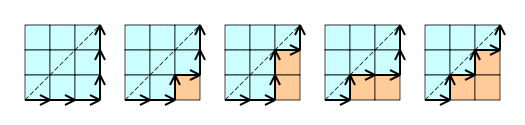
\includegraphics[width=0.4\paperwidth]{./img/catalan}
		\caption{\label{fig:catalan} Retículo de tamaño $\left(k,k\right)$.}
	\end{figure}
\end{example}

\begin{example}[La escalera]
	Un niño decide escalar una escalera con $n\geq 1$ de tal manera que cada paso que él despeja uno o dos de los pasos de la escalera %(vea)
	Encuentre la relación de recurrencia que sirva para calcular el número de diferentes maneras posibles de escalar la escalera.
\end{example}
Usamos la variable desconocida $x_{n}$ para denotar el número de maneras en las cuales el niño puede escalar la escalera de $n\geq1$ pasos. Es fácil de observar que $x_{1}=1$ y $x_{2}=2$ (dos pasos cada uno de longitud uno, o un paso de longitud dos escalones). Ahora sea $n\geq3$: si con el primer paso el niño mueve solo el primer escalón; existen claramente $x_{n-1}$ posibles maneras de escalar los que quedan. Si en cambio con el primer lugar, se suben dos peldaños de escalera.
\include{./03_mainmatter/fundament/exercise}
\textit{Resolver una ecuación de recurrencia} significa encontrar una sucesión que satisfaga las ecuaciones de recurrencias. Encontrar una ``solución general'' significa hallar una fórmula que describa todas las soluciones posibles (todas las sucesiones posibles que satisfacen la ecuación). Veamos el siguiente ejemplo:

\begin{example}
	Considere que $T_{n}$ satisface la siguiente ecuación para todo $n\in\mathds{N}$, $n>1$:
	\begin{equation*}
	T_{n}=2T_{n-1}+1.
	\end{equation*}
	La ecuación de recurrencia $T_{n}$ indica cómo continúa la sucesión pero no nos dice como empieza tal. % TODO: Crear una tabla de valores.
	\begin{itemize}
		\item Si $T_{1}=1$, se tiene $T=\left(1,7,3,15,31,\ldots\right)$.
		\item Si $T_{2}=1$, se tiene $T=\left(2,5,11,23,47,\ldots\right)$.
		\item Si $T_{4}=1$, se tiene $T=\left(4,9,19,39,79,\ldots\right)$.
		\item Si $T_{-1}=1$, se tiene $T=\left(-1,-1,-1,1-1,-1,\ldots\right)$.
	\end{itemize}
	?`Existe alguna fórmula para cada una de estas sucesiones? ?`Existe una fórmula en términos de $n$ y $T_{1}$ que describa todos los términos de la sucesión? ?`Existe una posible solución para $T_{n}$? Para poder responder este tipo de problemas, veamos un poco más de ecuaciones con recurrencia.
\end{example}

\section{Ejemplos definidos por ecuaciones de recurrencia}

\begin{example}[Parejas desordenadas]
	Imagina una fiesta donde las parejas llegan juntas, pero al final de la noche, cada persona se va con una nueva pareja. Para cada $n\in P$, digamos que $D_{n}$ es el número de diferentes formas en que las parejas pueden ser ``desordenadas'', es decir, reorganizadas en parejas, por lo que ni uno está emparejado con la persona con la que llegaron.

	Para los valores:
	\begin{itemize}
		\item $D_{1}=0$, una pareja no puede ser desordenada.
		\item $D_{2} = 1$, existe una y solo una manera de ``desordenar'' una pareja.
		\item $D_{3} = 2$, si las parejas llegan como $Aa$, $Bb$, $Cc$, entonces $A$ estaría emparejado con $b$ o $c$. Si $A$ esta emparejado con $b$, $C$ debe estar emparejado con $a$(y no $c$) y $B$ con $c$. Si $A$ esta emparejado con $c$, $B$ no debe estar emparejado con $a$(y no $b$) y $C$ con $b$.
	\end{itemize}
	?`Qué tan grandes son $D_{4}$, $D_{5}$ y $D_{10}$? ?`Cómo podemos calcularlos? ?`Existe alguna expresión cerrada para obtener todos los términos de la? % TODO: Sucesión.

	Vamos a desarrollar una estrategia para contar los desajustes cuando $n\leq4$. Supongamos que hay $n$ mujeres $A_{1},A_{2},A_{3},\ldots,A_{n}$, y cada $A_{j}$ llega con el hombre $a_{j}$.

	La mujer $A_{1}$ puede ser ``re-emparejada'' con cualquiera de los $n-1$ hombres restantes $a_{2}$ o $a_{3}$ o \ldots o $a_{n}$. Digamos que está emparejada con $a_{k}$, donde $2\leq k\leq n$ y ahora consideremos $a_{k}^{\prime}$ pareja original de la mujer $A_{k}$: ella podría tomar $a_{1}$ o ella podría rechazar $a_{1}$ y tomar a alguien más.

	Si $A_{1}$ es pareja con $a_{k}$ y $A_{k}$ es pareja con $a_{1}$, entonces $n-2$ parejas dejaron para desordenar, y eso puede hacerse exactamente de $D_{n-2}$ maneras diferentes.
	% TODO: Cambiar hacerse.

	Ahora para cada uno de los $n-1$ hombres que $A_{1}$ podría elegir, hay $\{D_{n-2}+ D_{n-1}\}$ diferentes formas de completar el trastorno. Por lo tanto, cuando $n\geq 4$ tenemos:
\begin{equation}\label{eq:1_1}
D_{n}=\left(n-1\right)\left\{D_{n-2}+D_{n-1}\right\}
\end{equation}
Usando la ecuación \eqref{eq:1_1} las evaluaciones para $n=1$ y $n=2$ verifican la igualdad, ahora evaluemos $D_{n}$ para cualquier valor de $n$, con $n\in\mathds{N}$
\begin{align*}
D_{3}&=\left(3-1\right)\left\{D_{2}+D_{1}\right\}=2\left(1+8\right)=2.\\
D_{4}&=\left(4-1\right)\left\{D_{3}+D_{2}\right\}=3\left(2+1\right)=9.\\
D_{5}&=\left(5-1\right)\left\{D_{4}+D_{3}\right\}=4\left(9+2\right)=44.\\
D_{6}&=(6-1)\left\{D_{5}+D_{4}\right\}=5\left(44 + 9\right)=265.\\
D_{7}&=\left(7-1\right)\left\{D_{6}+D_{5}\right\}=6\left(265+44\right)=1854.\\
D_{8}&=\left(8-1\right)\left\{D_{7}+D_{6}\right\}=7\left(1854+265\right)=14833.\\
D_{9}&=\left(9-1\right)\left\{D_{8}+D_{7}\right\}=8\left(14833+1854\right)=133496.\\
D_{10}&=\left(10-1\right)\left\{D_{9}+D_{8}\right\}=9\left(133496+14833\right)=1334961.
\end{align*}
La sucesión en $P$ definido por $S_{n}=A\times n!$ donde $A$ es un número real satisface la ecuación de recurrencia \eqref{eq:1_1}. Si $n\geq3$ se tiene:
\begin{align*}
	\left(n-1\right)\left\{S_{n-2}+S_{n-1}\right\}
	&=(n-1)\{A(n-2)!+A(n-1)!\} \\
	&=(n-1)A(n-2)!\{1+(n-1)\} \\
	&=A(n-1)(n-2)!\{n\}\\
	&=A\times n!\\
	&=S_{n}.
\end{align*}
?`Es válida la fórmula para $n=1$ o $n=2$? ?`Existe algún número real tal que $D_{n}=A(n!)$ cuando $n=1$ o $n=2$? No, porque si $0=D_{1}=A(1!)$, entonces $A$ debe ser igual a $0$, y si $1=D_{2}=A(2!)$, se tiene que $A$ debería tomar el valor de $\frac{1}{2}$. Sin embargo, podemos usar esta fórmula para probar que $D_{n}$ es acotado.
\end{example}

\begin{theorem}{}
Para todo $n\geq 2$, $\left(\frac{1}{3}\right)n!\leq D_{n}\leq\left(\frac{1}{2}\right)n!$.
\end{theorem}

\begin{proof}
	Primero considere la tabla de valores:
	\begin{table}[ht!]
		\centering
		\begin{tabular}{ >{$}c<{$} >{$}c<{$} >{$}c<{$} >{$}c<{$}}
			n & \left(\frac{1}{3}\right)n! & D_{n} & \left(\frac{1}{2}\right)n! \\
			\hline
			1 & \frac{1}{3} & 0 & \frac{1}{2}\\
			2 & \frac{2}{3} & 1 &  1=\frac{2}{2}\\
			3 & \frac{6}{3}=2 & 2 & 3=\frac{6}{2}\\
			4 & \frac{24}{3}=8 & 9 & 12=\frac{24}{2}\\
			5 & \frac{120}{3}=40 & 44 & 60=\frac{120}{2}\\
			6 & \frac{720}{3}=240 & 265 & 360=\frac{720}{2}\\
		\end{tabular}
	\end{table}
Por inducción fuerte en matemática sobre $n$.
\begin{enumerate}[label={Paso~\arabic*}]
	\item Si $n=2$, se tiene $\left(\frac{1}{3}\right)n!=\frac{2}{3}<1=D_{n}= \left(\frac{1}{2}\right)n!$ y $n=3$, se tiene $\left(\frac{1}{3}\right)n!=\frac{6}{3}=2=D_{n}<3=\left(\frac{1}{2}\right)n!$.
	\item Supongamos que $\exists k\geq3$ tal que si $2\leq n\leq k$, se tiene $\left(\frac{1}{3}\right)n!\leq D_{n}\leq\left(\frac{1}{2}\right)n!$.
	\item Si $n=k+1$, se tiene $n\geq 4$ y $D_{n}=(n-1)[D_{n-2}+D_{n-1}]$ cuando $2\leq n-2<n-1\leq k$. Así, $D_{n}\leq(n-1)\{(1/3)[n-2]!+(1/3)[n-1]!\}=(1/3)n!$, y $D_{n}\leq(n-1)\{(1/2)[n-2]!+(1/2)[n-1]!\}=(1/2)n!$.
\end{enumerate}
La mejor fórmula para $\bf{D_{n}}$ que sabemos utiliza la función de ``entero más cercano''. Para cualquier número real $x$, sea $\lceil x\rfloor$ que denote \emph{el entero más cercano a} $x$ se define de la siguiente manera:

\begin{itemize}
	\item Si $x$ es escrito como $n+f$ donde $n$ es el entero $\lfloor x\rfloor$, y $f$ es una fracción donde $0\leq f< 1$.
	\item Si $0 \leq f < \frac{1}{2}$, entonces $\lceil x\rfloor=n$.
	\item Si $\frac{1}{2}\leq f<1$, entonces $\lceil x\rfloor=n+1$.
\end{itemize}
?`Es $\lceil x\rfloor=\lfloor x+\frac{1}{2}\rfloor$? Así que $\lceil 3.29\rfloor=3$, $\lceil-3.78\rfloor=-4$. Entonces $D_{n}=\lceil(n!)/e\rfloor$ cuando $e=2.71828182844\ldots$ es la base del logaritmo natural. Note que $(n!)/e$ nunca es igual a $\lceil(n!)/e\rfloor+\frac{1}{2}$.

\begin{table}[ht!]
	\centering
	\begin{tabular}{>{$}c<{$} >{$}c<{$} >{$}c<{$}}
		n & D_{n} & (n!)/e \\
		\hline
		1 &  0 & 0.367879441\\
		2 &  1 &  0.735758882\\
		3 &  2 & 2.207276647\\
		4 &  9 & 8.829106588\\
		5 & 44 & 44.14553294\\
		6 & 265 & 264.8731976\\
		7 & 1854 & 1854.112384\\
		8 & 14833 & 14832.89907 \\
		9 & 133496 & 133496.0916\\
		10 &  1334961 & 1334960.916\\
	\end{tabular}
\end{table}

Hay otra fórmula (mucho menos compacta) para $D_{n}$ dado en los ejercicios, junto con un resumen de la prueba de que $D_{n}=\lceil(n!)/e\rfloor$.
\end{proof}

\begin{example}[Números de Ackermann]\index{Ackermann!número}
	En la década de 1920's, el lógico y matemático alemán, Wilhelm Ackermann (1896–1962), inventó una función muy curiosa, $A\colon P\times P\rightarrow P$ que se define recursivamente usando ``tres reglas'':
	\begin{enumerate}[label={Regla~\arabic*}]
		\item $A(1,n)=2$ para $n=1,2,\ldots$.
		\item $A(m,1)=2m$ para $m=2,3,\ldots$.
		\item Cuando $m>1$ y $n>1$ se tiene $A(m,n)=A(A(m-1,n),n-1)$.
	\end{enumerate}
\end{example}

Entonces,
\begin{align*}
A(2,2)
&=A(A(2-1,2),2-1)&\text{regla }3\\
&= A(A(1,2),1)&\\
&= A(2,1)&\text{regla }1\\
&= 2(2)&\text{regla }2\\
&= 4.
\end{align*}
Además
\begin{align*}
A(2,3)
&= A(A(2-1,3),3-1)&\text{regla }3\\
&= A(A(1,3),2)\\
&= A(2,2)&\text{regla }1\\
&= 4.
\end{align*}
De hecho, si $A(2,k)= 4$, para algún $k\geq2$, entonces
\begin{align*}
A(2,k+1) &= A(A(2-1,k+1), (k+1)-1)&\text{regla }3\\
&=A(A(1,k+1),k)\\
&=A(2,k)&\text{regla }1\\
&=4.
\end{align*}
Así, tenemos por inducción matemática $A(2,n)=4$, $\forall n\geq1$.

Hasta ahora la tabla de los números de Ackermann se ve así:

\begin{table}[ht!]
	\centering
	\begin{tabular}{>{$}c<{$}| >{$}c<{$} >{$}c<{$} >{$}c<{$} >{$}c<{$} >{$}c<{$} >{$}c<{$} >{$}c<{$} >{$}c<{$} >{$}c<{$}}
		A & n=1 & n=2 & n=3 & n=4 & n=5 & n=6 & n=7 & n=8 & n=9 \\
		\hline
		m=1 & 2 & 2 & 2 & 2 & 2 & 2 & 2 & 2 & 2 \\
		m=2 & 4 & 4 & 4 & 4 & 4 & 4 & 4 & 4 & 4 \\
		m=3 & 6 &  &  &  &  &  &  &  &  \\
		m=4 & 8 &  &  &  &  &  &  &  &  \\
		m=5 & 10 &  &  &  &  &  &  &  &  \\
	\end{tabular}
\end{table}

Observamos que la segunda fila es de puro 4s. ?`Pero cómo es la segunda columna?
Si $A(k,2)=2^{k}$ para algunos $k\geq2$ se tiene
\begin{align*}
	A(k,2)=2^{k}
	&= A(A([k+1],2-1)&\text{regla }3\\
	&= A(A(k,2),1) &\\
	&= A(2^{k},1)&\\
	&= 2(2^{k})&\text{regla }2\\
	&= 2^{k+1}.
\end{align*}
Además,
\begin{align*}
	A(2,3)
	&=A(A(2-1,3),3-1)&\text{regla }3\\
	&=A(A(1,3),2)&\\
	&=A(2,2)&\text{regla }1\\
	&=4.
\end{align*}
Así, se tiene $\forall m\geq1:A(m,2)=2^{m}$. Ahora, ?`como son los otros valores?
\begin{align*}
	A(3,3)
	&= A(A(3-1,3),3-1)&\text{regla }3\\
	&= A(A(2,3), 2)  \\
	&=A(4,2)&\text{segunda fila}\\
	&=2^{4}&\text{segunda columna}\\
	&=16.&\\
\end{align*}

\begin{align*}
	A(4,3)
	&=A(A(4-1,3),3-1)&\text{regla }3\\
	&= A(A(3,3), 2) &\\
	&=A(16,2)&\text{encima}\\
	&=2^{16}&\text{segunda columna}\\
	&=65536.&\\
\end{align*}

\begin{align*}
	A(3,4)
	&= A(A(3-1,3),4-1)&\text{regla }3\\
	&= A(A(2,4), 3) &\\
	&=A(4,3)&\text{segunda fila}\\
	&=65536.&\\
\end{align*}
?`Cual es el valor de $A(4,4)$? ?`Podría ejecutar un programa recursivo simple para evaluar $A(4,4)$?
\begin{align*}
	A(5,3)
	&= A(A(5-1,3),3-1)&\text{regla }3\\
	&= A(A(4,3),2) &\\
	&=A(65536,2) &\\
	&=2^{65536}.&\text{segunda columna}\\
	&=n&\text{grande aproximadamente }20000\text{ dígitos en base }10.\\
\end{align*}
Hasta ahora tenemos:

\begin{table}[ht!]
	\centering
	\begin{tabular}{>{$}c<{$}| >{$}c<{$} >{$}c<{$} >{$}c<{$} >{$}c<{$} >{$}c<{$} >{$}c<{$} >{$}c<{$} >{$}c<{$} >{$}c<{$}}
		A & n=1 & n=2 & n=3 & n=4 & n=5 & n=6 & n=7 & n=8 & n=9 \\
		\hline
		m=1 & 2 & 2 & 2 & 2 & 2 & 2 & 2 & 2 & 2 \\
		m=2 & 4 & 4 & 4 & 4 & 4 & 4 & 4 & 4 & 4 \\
		m=3 & 6 & 8 & 16 & 65536 & \text{?} &  &  &  &  \\
		m=4 & 8 & 16 & 65536  & \text{?} &  &  &  &  &  \\
		m=5 & 10 & 2^{65536} &  &  &  &  &  &  &  \\
	\end{tabular}
\end{table}
?`Cómo continúa la tercera columna? Sea $2\uparrow$ denota el valor de ``Torre'' de k 2's, definida recursivamente por \[ 2\uparrow 1=2,\quad\text{y para}\quad k\geq1,\quad2\uparrow\left[k+1\right]=2^{2\uparrow k}. \]
Pero este es un número tan grande que nunca podría escribirse en dígitos decimales, incluso utilizando todo el papel del mundo, Su valor nunca podría ser calculado. Ahora nos preguntamos ?`Los números Ackermann son ``computables''? Por otro lado, supongamos que las sucesiones que encontramos, incluso aquellas definidas por ecuaciones de recurrencia, serán fáciles para entender y tratar.
\section{Resolución de ecuaciones de recurrencia lineal de primer orden}

Una ecuación de recurrencia lineal de primer orden relaciona entradas consecutivas en una secuencia por una ecuación de la forma:
\begin{equation}\label{eq:lineara}
S_{n+1}=a S_{n}+c\quad\text{ para todo }n\text{ en el dominio de } S.
\end{equation}
Una solución general es una descripción algebraica de todas estas secuencias de soluciones. Si $S$ es cualquier secuencia en $\mathds{N}$ que satisface la ecuación anterior, entonces denotando $S_{0}$ por $I$, tenemos:
\begin{align*}
S_1&=aS_0+c=aI+c \\
S_2=&aS_1+c=a[aI+c]+c=a^2I+ac+c \\
S_3=&aS_2+c=a[a^2I+ac+c]+c=a^3I+a^2c+ac+c
\end{align*}
Entonces podríamos decir que
\begin{equation}\label{eq:linearb}
S_n = a^nI+a^{n-1}c+a^{n-2}c +\cdots+ac+c\quad\text{para }\forall n\in\mathds{N}.
\end{equation}
Podemos demostrarlo por \emph{inducción matemática} para cualquier $n\in\mathds{N}$, $S_k=a^nI+a^{n-1}c+a^{n-2}c+\cdots+ac+c$, entonces:
\begin{align*}
S_{k+1}&=aS_{k} + c  \\
S_{k+1}&=a\left[a^kI+a^{k-1}c+a^{k-2}c+\cdots+ac+c\right] + c\\
S_{k+1}&=a^{k+1}I+a^k c+a^{k-1}c+\cdots+a^2c+ac+c
\end{align*}
Por lo tanto,~\eqref{eq:linearb} es correcto. Por lo tanto, si $S$ es cualquier secuencia en $\mathds{N}$ que satisface~\eqref{eq:lineara}, entonces para $\forall n\in \mathds{P}$.
\begin{itemize}
	\item Si $a=1$, entonces $S_n=1^nI+1^{n-1}c+1^{n-2}+\cdots+1c+c=I+nc$.
	\item Y si $a\neq1$, se tiene
	\begin{align*}
	S_n&=a^{n}I+a^{n-1}c+a^{n-2}c+\cdots+ac+c\\
	&=a^{n}I+c\frac{1-a^n}{1-a}=a^nI+\frac{c}{1-a}-a^n\frac{c}{1-a}\\
	&=a^{n}\left[1-\frac{c}{1-a}\right]+\frac{c}{1-a}\\
	\end{align*}
\end{itemize}
Por lo tanto, la solución general a la ecuación de recurrencia es \[ S_{n+1} = aS_n+c,\quad\forall n\in\mathds{N}. \] Se da en dos partes:
\begin{align*}
\text{Si }a=1, S_n&= S_0+ nc,\quad\forall n\in\mathds{N}\\
\text{Si }a\neq1&=S_n= a^{n}\left[S_0-\frac{c}{1-a}\right]+\frac{c}{1-a}\forall n\in\mathds{N}.
\end{align*}

\subsection{Las torres de Hanói}\index{Torres de Hanói}

Cuenta la leyenda que los monjes de un monasterio de la ciudad Hanói medían el tiempo que faltaba para la llegada del ``fin del mundo'' con el siguiente procedimiento:
\begin{quote}
	``Se dispone de tres agujas de diamante, en una de las cuales se apilan $64$ discos de oro distintos, ordenados según el tamaño de sus diámetros. En cada segundo mueven un disco de una aguja a otra, y su tarea finalizará (y con ella el mundo) cuando logren transportar todos los discos a la otra aguja. Pero, ¡atención!, a lo largo del proceso no se puede colocar un disco sobre otro de diámetro más pequeño.''.
\end{quote}
Como la preparación para el ``fin del mundo'' supondrá sin duda un notable ajetreo, vamos a estimar el tiempo del cuál dispondremos. Por ello, replanteamos el problema en general:
\begin{quote}
	``Tenemos $n$ discos y llamamos $a_n$ al mínimo número de movimientos necesario para transportar los $n$ discos desde una aguja a otra.''.
\end{quote}
Por ejemplo, si $a_{1}=1$, nos basta con un movimiento para pasar el disco a otra aguja. El cálculo de $a_2$ requiere ya un pequeño argumento: podemos, por ejemplo, pasar el disco pequeño a otra aguja, luego el grande a la tercera, para finalmente pasar el pequeño a esta tercera aguja, como en la figura~\ref{fig:hanoi}
\begin{figure}[ht!]
	\sidecaption[t]%[ht!]
	\centering
	
\includegraphics[width=0.4\paperwidth]{./img/hanoi}
	\caption{\label{fig:hanoi} Proceso exitoso para dos discos.}
\end{figure}
Como en dos movimientos no se puede hacer, concluimos que la descrita es la mejor estrategia posible, y que, por tanto, $a_{2}= 3$. Si partimos de tres discos, podemos pasar los dos menores a una segunda aguja (con el procedimiento anterior, de tres movimientos), luego pasar el mayor a la tercera aguja, para finalmente llevar los dos discos menores sobre ese disco mayor (de nuevo tres movimientos). En total, $7$ movimientos. Aunque ahora no está claro si se puede hacer el trasvase con menos.

El procedimiento esbozado en el caso $n=3$ se puede generalizar: si tenemos $n$ discos, pasamos $n-1$ a una segunda aguja, luego el mayor disco a la aguja final y, por último, pasamos los $n-1$ discos a esa tercera aguja. Es un algoritmo recursivo: el procedimiento para mover $n$ discos se apoya, dos veces, en el (ya conocido) método para mover $n-1$. Se deduce entonces que el número mínimo de movimientos para transportar $n$ discos cumple que
\begin{equation}\label{eq:hanoi1}
	a_{n}\leq 2a_{n-1}+1,\quad\forall n\geq2
\end{equation} porque con $2a_{n-1}+1$ movimientos lo sabemos hacer. Observe que no es una ecuación de recurrencia, sino una desigualdad. Para comprobar que, en realidad, la
relación se cumple en la igualdad. Deduciríamos así que la estrategia de movimientos es la mejor posible. Esto requiere un argumento extra.

Veamos: Si tenemos $n$ discos, en algún momento tendremos que mover el disco mayor, para lo que necesitaremos haber llevado el resto de los discos a otra aguja, pues debe quedar una aguja libre. Esto requiere, como mínimo $a_{n-1}$ movimientos. Una vez movido el disco grande a una aguja, tendremos que mover los restantes $n-1$ discos sobre él, y esto exige, al menos, otros $a_{n-1}$ movimientos (sea cual sea la estrategia que empleemos). Así que
\begin{equation}\label{eq:hanoi2}
	a_{n}\geq 2a_{n-1}+1,\quad\forall n \geq 2.
\end{equation}
Reuniendo las condiciones~\eqref{eq:hanoi1} y~\eqref{eq:hanoi2}, ya podemos afirmar que
\begin{equation}
	a_{n}= 2a_{n-1}+1,\quad\forall n\geq2.
\end{equation}
La condición inicial ya la hemos visto, es $a_{1}=1$. La resolvemos por simple aplicación repetida de la regla de recurrencia:
\begin{align*}
	a_{n}&=2a_{n-1}+1=2\left(2a_{n-2}+1\right)+1=2^{2}a_{n-2}+2+1=2^{2}\left(2a_{n-3}+1\right)+2+1\\
	a_{n}&= 2^{3}a_{n-3}+2^{2}+2+1=2^{3}(2a_{n-4}+1)+2+1=2^{4}a_{n-4}+2^{3}+2^{2}+2+1\\
	a_{n}&=2^{n-1}a_{1}+2^{n-2}+2^{n-3}+\cdots+2+1=\sum_{k=1}^{n}2^{k-1}=\frac{1-2^{n}}{1-2}=2^{n}-1.
\end{align*}
En el caso de $n=64$ deducimos que el fin del mundo llegará dentro de $a_{64}= 2^{64}-1$ segundos, esto es, !`más de medio billón de años! Parece que, después de todo, la profecía de los monjes de Hanói no debería ser una de nuestras mayores preocupaciones.

\begin{example}{Recurrencia del número de movimientos en la Torre de Hanói}
	La ecuación de recurrencia para el número de movimientos en las Torres de Hanói es una ecuación de recurrencia lineal de primer orden:
	\begin{equation*}
	T_{n}=2T_{n-1}+1.
	\end{equation*}
	Sea $a=2$ y $c=1$, entonces $\frac{c}{1-a}=\frac{1}{1-2}=-1$, y cualquier secuencia $T$ que satisfaga la $RE$ está dado por la fórmula:
	\begin{align*}
	T_{n}&=2^{n}\left[T_{0}-(-1)\right]+(-1)\\
	T_{n}&=2^{n}\left[T_{0}+1\right]-1
	\end{align*}
	Asumiendo que $T$ tiene el dominio $\mathds{Z}$ y que denota $T_0$ la condición inicial, vimos al principio de este capítulo varias soluciones particulares:
	\begin{align*}
		\text{Si }T_{0}=0,\text{ entonces }T=\left(0,1,3,7,15,31,\ldots\right)\quad &T_{n}=2^{n}[0+1]-1=2^n-1.\\
		\text{Si }T_{0}=2,\text{ entonces }T=\left(4,9,19,39,79,159,\ldots\right)\quad &T_{n}=2^{n}[2+1]-1=3\times2^{n}-1.\\
		\text{Si }T_{0}=4,\text{ entonces }T=\left(2,5,11,23,47,95,\ldots\right)\quad &T_{n}=2^{n}[4+1]-1=5\times2^{n}-1.\\
		\text{Si }T_{0}=-1,\text{ entonces }T=\left(-1,-1,-1,-1,-1,\ldots\right)\quad &T_{n}=2^{n}\left[-1+1\right]-1=-1.
	\end{align*}
\end{example}

\subsection{Los tres piratas naufragados}

Un barco pirata es naufragado en una tormenta en la noche. Tres de los piratas sobreviven y se encuentran en una playa la mañana después de la tormenta. Aceptan cooperar para asegurar su supervivencia. Ellos divisan a un mono en la selva cerca de la playa y pasan todo ese primer día recogiendo una gran pila de cocos y luego se van a dormir exhaustos. Pero ellos son piratas. El primero duerme bien, preocupado por su parte de los cocos; despierta, divide la pila en 3 montones iguales, pero encuentra uno sobrante que arroja en el arbusto para el mono, entierra su tercero en la arena, amontona los otros dos montones, y se va a dormir profundamente. El segundo pirata duerme bien, preocupado por su parte de los cocos; se despierta, divide la pila en 3 montones iguales, pero encuentra uno sobrante que arroja en el arbusto para el mono, entierra su tercero en la arena, amontona los otros dos montones, y se va a dormir profundamente.

El tercero también duerme bien, preocupado por su parte de los cocos; despierta, divide la pila en 3 montones iguales, pero encuentra uno sobrante que arroja en el arbusto para el mono, entierra su tercero en la arena, amontona los otros dos montones juntos, y se va a dormir profundamente.

A la mañana siguiente, todos se despiertan y ven una pila algo más pequeña de cocos que se dividen en 3 montones iguales, pero encontrar uno sobrante que tiran en el arbusto para el mono. ?`Cuántos cocos recolectaron el primer día?

Sea $S_{j}$ el tamaño de la pila después del pirata $j^{4h}$ y sea $S_{0}$ el número que recogieron en el primer día. Entonces
\begin{align*}
	S_{0}&=3x+1\text{ para algún número entero }x\text{ y }S_1=2x,\\
	S_{1}&= 3y+1\text{ para algún número entero }y\text{ y }S_2=2y,\\
	S_{2}&=3z+1\text{ para algún número entero}z\text{ y }S_3=2z,\\
	\intertext{y}
	S_{3}&=3w+1\text{ para algún número entero }w.
\end{align*}
?`Hay una ecuación de recurrencia aquí?
\begin{align*}
	S_{1}&=2x\text{ donde }x=(S_{0}-1)/3\text{, entonces }S_{1}=(2/3)S_0-(2/3)\\
	S_{2}&=2y\text{ donde }y=(S_{1}-1)/3\text{, entonces }S_{2}=(2/3)S_1-(2/3)\\
	S_{3}&=2z\text{ donde }z=(S_{2}-1)/3\text{, entonces }S_{3}=(2/3)S_2-(2/3).
\end{align*}
La ecuación de recurrencia satisfecha por los primeros $S_{j}^{\prime}s$ es
\begin{equation}
	S_{j+1}=(2/3)S_{j}-(2/3).
\end{equation}
Si ahora tenemos $S_{4}=(2/3)S_{3}-(2/3)$, entonces $S_{4}=2[S_{3}-1]/3=2w$ para algún número entero $w$. Queremos saber qué valor (o valores) de $S_0$ producirá un número entero par para $S_4$ cuando aplicamos el RE (1). En (1), $a=2/3$ y $c=-2/3$, entonces $c/(1-a) = -2$, y así la solución general de (1) es
\begin{equation*}
	S_{n}={\left(\frac{2}{3}\right)}^{n}\left[S_{0}+2\right]-2.
\end{equation*}
Por lo tanto, $S_{4}=(2/3)^{4}[S_0+2]-2=(16/81)\left[S_0 + 2\right]-2$.

$S_{4}$ será un número entero

$\Leftrightarrow S_{4}+2$ es (un aún) el número entero

$\Leftrightarrow 81\divides\left[S_0 + 2\right]$

$\Leftrightarrow\left[S_{0}+2\right]= 81k$ para algún número entero $k$

$\Leftrightarrow S_{0}=81k-2$ para algún número entero $k$.

$S_{0}$ debe ser un número entero positivo, pero hay un número infinito de respuestas posibles: \[ 79\vee160\vee241\vee322\vee\cdots \]

Necesitamos más información para determinar $S_0$. Si nos hubieran dicho que el primer día los piratas recolectaron entre $200$ y $300$ cocos, ahora podríamos decir ``el número que recogieron el primer día fue exactamente $241$''.

\subsection{Interés compuesto}\index{Interés compuesto}

Supongamos que se le ofrecen dos planes de ahorro para la jubilación. En el plan $A$, empiezas con $\$1,000$, y cada año (en el aniversario del plan), te pagan un $11\%$ de interés simple, y agregas $\$1,000$. En el plan $B$, empiezas con $\$100$, y cada mes, te pagan una-duodécima parte del $10\%$ de interés simple (anual), y agregas $\$100$. ?`Qué plan será más grande después de $40$ años?. ?`Podemos aplicar una ecuación de recurrencia? Considere el plan A y deje que $S_{n}$ denote el número de dólares en el plan después de (exactamente) $n$ años de operación. Entonces $S_{0}=\$1,000$ y
\begin{align*}
	S_{n+1}&= S_{n}+\text{ interés sobre }S_n+\$1000\\
	S_{n+1}&=S_{n}+11\%\text{ de }S_n+\$1000\\
	S_{n+1}&=S_{n}(1+0.11)+\$1000.
\end{align*}
En esta RE, $a=1.11$, $c=1000$, entonces $\frac{c}{1-a}=\frac{1000}{-0.11}$ y
\begin{align*}
	S_{n}&={\left(1.11\right)}^{n}\left[1000-\frac{1000}{-0.11}\right]+\frac{1000}{+0.11}\\
	S_{n}&={\left(1.11\right)}^{n}\left[\frac{1110}{+0.11}\right]-\frac{1000}{+0.11}
\end{align*}
Por lo tanto,
\begin{align*}
	S_{40}&={\left(1.11\right)}^{40}(10090.090909\ldots)-(-9090.909090\ldots)\\
	S_{40}&=(65.000867\ldots)(10090.090909\ldots)-(9090.909090\ldots)\\
	S_{40}&=655917.842\ldots-(9090.909090\ldots)\\
	S_{40}&\approx\$646826.
\end{align*}
?`Puede ser cierto? Pusiste $\$40000$ y sacaste mayor que $\$600000$ en intereses. Ahora considere el plan $B$ y sea $T_{n}$ denota el número de dólares en el plan después de (exactamente) $n$ meses de funcionamiento. Entonces $T_{0}=\$100$ y
\begin{align*}
	T_{n+1}&=T_{n}+\text{ interés sobre }T_{n}+\$100\\
	T_{n+1}&= T_{n}+\left(\frac{1}{2}\right)\text{ de }10\%\text{ de }T_{n}+\$100\\
	T_{n+1}&=T_{n}\left[1+\frac{0.1}{12}\right]\$100
\end{align*}
En esta RE, $a=12.1/12,c=100$, entonces $\frac{c}{1-a}=\frac{100}{-0.1/12}=-12000$ y
\begin{equation*}
	T_{n}={\left(\frac{12.1}{12}\right)}^{n}\left[100+12000\right]-12000.
\end{equation*}
De ahí, después $40\times12$ meses,
\begin{align*}
	T_{480}&={\left(\frac{12.1}{12}\right)}^{480}(12100)-(12000)\\
	T_{480}&={\left(1.008333\ldots\right)}^{480}(12100)-(12000)\\
	T_{480}&=\left(53.700663\ldots\right)(12100)-(12000)\\
	T_{480}&=649778.0234\ldots-(12000)\\
	T_{480}&\approx\$637778.
\end{align*}
Por lo tanto, el plan $A$ tiene un valor ligeramente mayor después de $40$ años.

\section{Resolución de ecuaciones de recurrencia lineal de segundo orden}

Una \emph{ecuación de recurrencia lineal de segundo orden} relaciona entradas consecutivas en una secuencia por una ecuación de la forma
\begin{equation}\label{eq:segordena}
	S_{n+2}=aS_{n+1}+bS_{n}+c\quad\forall n\text{ en el dominio de }S.
\end{equation}
Pero vamos a asumir que el dominio de $S$ es $\mathds{N}$. Supongamos también que $ab\neq0$, de lo contrario, $S_{n}=c$ para $\forall n\in\left\{2\ldots\right\}$, y las soluciones de~\eqref{eq:segorden} no son muy interesantes.

\begin{remark}
	La ecuación de recurrencia de primer orden es solo un caso especial de la ecuación de recurrencia de segundo orden~\eqref{eq:segorden} cuando $b=0$.
\end{remark}

Cuando $c=0$, se dice que la RE es \textbf{homogénea} (todos los términos lucen igual a una constante multiplicada por una sucesión).

\begin{remark}
	La ecuación de recurrencia de Fibonacci es homogénea.
\end{remark}

Vamos a restringir también nuestra atención (por el momento) a una \emph{lineal de segundo orden}, la \emph{ecuación de recurrencia homogénea}
\begin{equation}\label{eq:segordenb}
	S_{n+2}=aS_{n+1}+bS_{n}\text{ para }\forall n\in\mathds{N}.
\end{equation}
Tal como hicimos para la ecuación de la recurrencia de Fibonacci, supongamos que existe una secuencia geométrica, $S_{n}=r^{n}$, que satisface~\eqref{eq:segordenb}. Si lo hubiera, entonces \[ r^{n+2}=ar^{n+1}+br^{n},\quad\forall n\in\mathds{N}. \] Cuando $n=0$, \[ r^{2}=ar+b. \]

La ``ecuación característica'' de~\eqref{eq:segordenb} es $x^2-ax-b=0$, cuyas ``raíces'' son \[ r=\frac{-\left(-a\right)\pm\sqrt{{\left(-a\right)}^{2}-4\left(1\right)\left(-b\right)}}{2\left(1\right)}=\frac{a\pm\sqrt{a^{2}+4b}}{2}. \]

Sean $\Delta=\sqrt{a^2+4b}$, $r_1=\frac{a+\Delta}{2}$, y $r_2=\frac{a-\Delta}{2}$, entonces $r_{1}+r_{2}=a$, $r_{1}\times r_{2}=-b$, y $r_{1}-r_{2}=\Delta$. Tanto $r_{1}$ como $r_{2}$ satisfacen la ecuación $x^{2}=ax+b$, y son las únicas soluciones.

\begin{example}{}
Si $S_{n+2}=10S_{n+1}-21S_n$ para $\forall n\in\mathds{N}$, la ecuación característica es $x^{2}-10x+21=0$ o $(x-7)(x-3)=0$.

Aquí $a=10$, $b=-21$, $a^2+4b=100-84=16$, $\Delta = 4$, entonces $r_{1}=7$ y $r_{2}=3$.
\end{example}

\begin{example}{}
Si $S_{n+2} = 3S_{n+1}-2S_{n}$ para $\forall n\in\mathds{N}$, la ecuación característica es $x^{2}-3x+2=0$ o $(x-2)(x-1)=0$.

Aquí, $a=3$, $b=-2$, $a^{2}+4b=9-8=1$, $\Delta = 1$, entonces $r_{1}=2$ y $r_{2}=1$.
\end{example}

\begin{example}{}
Si $S_{n+2}=2S_{n+1}-S_{n}$ para $\forall\,n\in\mathds{N}$, la ecuación característica es $x^{2}-2x+1=0$ o $(x-1)(x-1)=0$.

Aquí, $a=2$, $b=-1$, $a^2+4b=4-4=0$, $\Delta = 0$, entonces $r_{1}=1$ y $r_{2}=1$.
\end{example}

?`Pero qué hay de una fórmula que da la solución general?

\begin{theorem}
La solución general de la RE homogénea~\eqref{eq:segordenb} es
	\begin{align*}
		S_{n}&=A(r_1)^{n}+B(r_2)^{n},&\text{si }r_{1}\neq r_{2}\left(\Delta\neq0\right)&
		\shortintertext{y}
		S_{n}&=A(r)^n+Bn(r)^{n},&\text{si }r_{1}=r_{2}=r\left(\Delta=0\right).&
	\end{align*}
\end{theorem}
\begin{proof}
Supongamos que $T$ es cualquier solución particular de la RE homogénea. Nos ocupamos de los dos casos por separado.
\begin{enumerate}[label={Caso~\arabic*}]
	\item Si $\Delta\neq0$, entonces las dos raíces son distintas (pero pueden ser números ``complejos''). Encontraremos valores para $A$ y $B$, luego probaremos que $T_{n}=A(r_1)^{n}+B(r_2)^{n}$ para $\forall\,n\in\mathds{N}$. Mostraremos que $A(r_1)^{n}+B(r_2)^{n}$ inicia correctamente para valores especialmente elegidos de $A$ y $B$, y luego mostraremos que $A(r_1)^{n}+B(r_2)^{n}$ continúa correctamente.

	Vamos a resolver las ecuaciones (para $A$ y $B$) que garantizaría $T_{n}=A(r_1)^{n}+B(r_{2})^n$, entonces $n=0$ y $n=1$. Si
		\begin{align}
		T_{0}&={A(r_{1})}^{0}+{B(r_{2})}^{0}=A+B\label{eq:sol1}
		\shortintertext{y}
		T_{1}&={A(r_{1})}^{1}+{B(r_{2})}^{1}=A(r_{1})+B(r_{2}),\label{eq:sol2}
		\end{align}
	entonces $(r_{1})T_{0}=A(r_{1})+B(r_{1})$. multiplicamos~\eqref{eq:so} por $r_{1}$ y $T_{1}= A(r_{1})+B(r_{2})$// (2) otra vez restamos, obtenemos $(r_{1})T_{0}-T_{1}=B(r_{1}-r_{2})=B\Delta$//$r_{1}-r_{2}=\Delta\neq 0$ entonces $B=\frac{(r_{1})T_{0}-T_{1}}{\Delta}$. Tenemos, $A=T_{0}-B=\frac{\Delta T_{0}}{\Delta} -\frac{(r_{1})T_{0}-T_{1}}{\Delta}=\frac{-(r_{2})T_{0}+T_{1}}{\Delta}$. No importa cómo comience la sucesión $T$ (no importa cuáles sean los valores para $T_{0}$ y $T_{1}$). Hay números únicos $A$ y $B$ tales que $T_{n}={A(r_{1})}^{n}+{B(r_{2})}^{n}$ para $n=0$ y $1$. Continuando la prueba por la inducción matemática que $T_{n}={A(r_{1})}^{n}+{B(r_{2})}^{n}$ para $\forall n\in\mathds{N}$.

	\begin{enumerate}[label={Paso~\arabic*}]
		\item Si $n=0$ o $n=1$, entonces $T_{n} = A(r_{1})^{n}+B(r_{2})^{n}$, por nuestra ``opción'' $A$ y $B$.
		\item Asuma que $\exists k\geq1$ tal que si $0\leq n\leq k$, entonces $T_{n}={A(r_{1})}^{n}+{B(r_{2})}^{n}$.
		\item Si $n=k+1$, entonces $n\geq2$ entonces, porque $T$ satisface la RE homogénea (3).
	\end{enumerate}
	\begin{align*}
		T_{k+1}&=aT_{k}+bT_{k-1}\\
		T_{k+1}&=a\left[A(r_1)^k + B(r_2)^k\right]+b\left[A(r_1)^{k-1} + B(r_2)^{k-1}\right] \text{por el paso }2\\
		T_{k+1}&=\left[aA(r_1)^k+bA(r_1)^{k-1}\right]+[aB(r_2)^k+bB(r_2)^{k-1}]\\
		T_{k+1}&=A(r_1)^{k-1}[a(r_1)+b]+B(r_2)^{k-1}[a(r_2)+n]\\
		T_{k+1}&= A(r_1)^{k+1}+B(r_2)^{k+1}
	\end{align*}
	Así, si $r_{1}\neq r_{2}$, $T_{n}=A(r_1)^n+B(r_2)^n$ para $\forall\,n\in\mathds{N}$.
	% TODO: Checkear bien escrito.
	\begin{example}{}
	Si $S_{n+2}=10S_{n+1}-21S_{n}$ para $\forall\, n\in\mathds{N}$, entonces $r_{1}=7$ y $r_{2}=3$. Tenemos, la solución general de la RE es $S_{n}=A7^n+B3^{n}$.
	\end{example}

	\begin{example}{}
	Si $S_{n+2}=3S_{n+1}-2S_{n}$ para $\forall n\in\mathds{N}$, entonces $r_{1}=2$ y $r_{2}=1$. Tenemos, la solución general de la RE es $S_{n}= A2^{n}+B1^{n}=A2^{n}+B$.
	\end{example}
\item Si $\Delta=0$, entonces las raíces son (ambos) iguales a $r$ donde $r=a/2$. También, $b=-a^{2}/4=-r^{2}$. Si $a$ eran $0$, entonces $b=0$, pero asumimos que no tanto $a$ y $b$ son $0$. De ahí, $r\neq0$. Vamos a resolver las ecuaciones (para $A$ y $B$) que garantizarían $T_{n}=A{\left(r\right)}^{n}+nB{\left(r\right)}^{n}$ cuando $n=0$ y $n=1$. Si
\begin{align}
	T_{0}&={A(r)}^{0}+0{B(r)}^{0}=A%(1)
	\intertext{y}
	T_{1}&={A(r)}^{1}+1{B(r)}^{1}=Ar+Br%(2)
\end{align}
entonces $A=T_{0}$ y $B=(T_{1}-Ar)/r$. No importa cómo comience la sucesión $T$ (no importa cuáles sean los valores para $T_{0}$ y $T_{1}$). Hay números únicos $A$ y $B$ tales que $T_n = A(r)^n + B(r)^n$ para $n = 0$ y $1$. Continuando la prueba por la inducción matemática que $T_{n}={A(r)}^{n}+{B(r)}^{n}$ para $\forall n\in\mathds{N}$.

\begin{enumerate}[label={Paso~\arabic*}]
	\item Si $n=0$ o $n=1$, entonces $T_{n}={A(r)}^{n}+{B(r)}^{n}$, por nuestra ``opción'' $A$ y $B$.
	\item Asuma que $\exists k\geq1$ tal que si $0\leq n\leq k$, entonces $T_{n}={A(r)}^{n}+{B(r)}^{n}$.
	\item Si $n=k+1$, entonces $n\geq2$ entonces, porque $T$ satisface la RE homogénea (3).
\end{enumerate}

\begin{align*}
	T_{k+1}&= aT_{k}+bT_{k-1}\\
	T_{k+1}&= a[A(r)^k+kB(r)^k]+b[A(r)^{k-1}+(k-1)B(r)^{k-1}] // \text{ por el paso 2}\\
	T_{k+1}&=[aAr^k+bAr^{k-1}]+[akBr^k+b(k-1)Br^{k-1}]\\
	T_{k+1}&=Ar^{k-1}[ar+b]+Br^{k-1}[akr + b(k-1)]\\
	T_{k+1}&=Ar^{k-1}[r^2]+Br^{k-1}[k(r^{2}) +r^{2}]//r^2 = ar + b\\
	T_{k+1}&=Ar^{k+1}+Br^{k-1}[k(r^2) + r^2]//-b = r^{2}\\
	T_{k+1}&=Ar^{k+1}+(k+1)Br^{k+1}
\end{align*}

Así, si $r_{1}=r_{2}=r$, $T_{n}=A(r)^{n}+nB(r)^{n}$ para $\forall n\in\mathds{N}$.
\end{enumerate}
\end{proof}
%\motto{Use the template \emph{chapter.tex} to style the various elements of your chapter content.}
\chapter{}
\label{intro} % Always give a unique label
 use \chaptermark{}
 to alter or adjust the chapter heading in the running head

\abstract*{}
%% Always give a unique label
%% and use \ref{<label>} for cross-references
%% and \cite{<label>} for bibliographic references
%% use \sectionmark{}
%%% to alter or adjust the section heading in the running head
%%
%%% For figures use
%%%
%\begin{figure}[!ht]
%	\sidecaption[t]
%	% Use the relevant command for your figure-insertion program
%	% to insert the figure file.
%	% For example, with the option graphics use
%	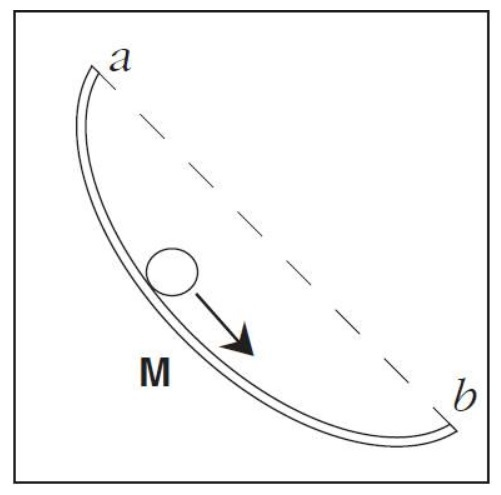
\includegraphics[width=0.343\textwidth]{bola.jpg}
%	%
%	% If not, use
%	%\picplace{5cm}{2cm} % Give the correct figure height and width in cm
%	%
%	\caption{Dados dos puntos $A$ y $B$, con $A$ a una elevación mayor que $B$, existe solo una curva cicloide con la concavidad hacia arriba que pasa por $A$ con pendiente infinita (dirección vertical y sentido de arriba hacia abajo), también pasa por $B$ y no posee puntos máximos entre $A$ y $B$.}
%	\label{fig:1}       % Give a unique label
%\end{figure}
%
%\eject
%
%%\begin{eqnarray}
%%\left|\nabla U_{\alpha}^{\mu}(y)\right| &\le&\frac1{d-\alpha}\int
%%\left|\nabla\frac1{|\xi-y|^{d-\alpha}}\right|\,d\mu(\xi) =
%%\int \frac1{|\xi-y|^{d-\alpha+1}} \,d\mu(\xi)\qquad  \\
%%&=&(d-\alpha+1) \int\limits_{d(y)}^\infty
%%\frac{\mu(B(y,r))}{r^{d-\alpha+2}}\,dr \le (d-\alpha+1)
%%\int\limits_{d(y)}^\infty \frac{r^{d-\alpha}}{r^{d-\alpha+2}}\,dr
%%\label{eq:01}
%%\end{eqnarray}
%
%\enlargethispage{24pt}
%
%\begin{quotation}
%Please do not use quotation marks when quoting texts! Simply use the \verb|quotation| environment -- it will automatically be rendered in the preferred layout.
%\end{quotation}
%\subsection{Algunas observaciones, demostraciones y aplicaciones de Euler, Lagrange y Jacobi en el Cálculo variacional}
%Instead of simply listing headings of different levels we recommend to let every heading be followed by at least a short passage of text. Furtheron please use the \LaTeX\ automatism for all your cross-references and citations as has already been described in Sect.~\ref{subsec:2}, see also Fig.~\ref{fig:1}\footnote{If you copy text passages, figures, or tables from other works, you must obtain \textit{permission} from the copyright holder (usually the original publisher). Please enclose the signed permission with the manucript. The sources\index{permission to print} must be acknowledged either in the captions, as footnotes or in a separate section of the book.}
%\paragraph{Paragraph Heading} %
%Instead of simply listing headings of different levels we recommend to let every heading be followed by at least a short passage of text. Furtheron please use the \LaTeX\ automatism for all your cross-references and citations as has already been described in Sect.~\ref{sec:2}.
%
%Please note that the first line of text that follows a heading is not indented, whereas the first lines of all subsequent paragraphs are.
%
%For typesetting numbered lists we recommend to use the \verb|enumerate| environment -- it will automatically render Springer's preferred layout.
%\begin{figure}[h]
%	\centering
%	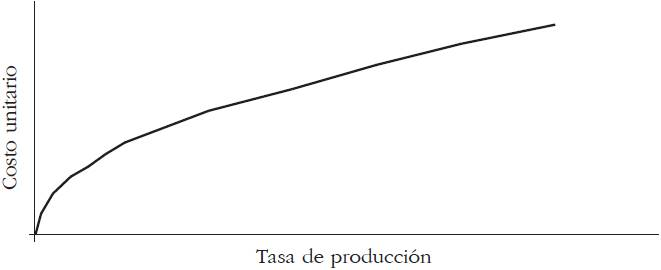
\includegraphics[width=0.6\textwidth]{grafica.jpg}
%	\caption{Costo de producción proporcional a la raíz cuadrada de la tasa de producción.}
%\end{figure}
%\begin{figure}[t]
%\sidecaption[t]
%% Use the relevant command for your figure-insertion program
%% to insert the figure file.
%% For example, with the option graphics use
%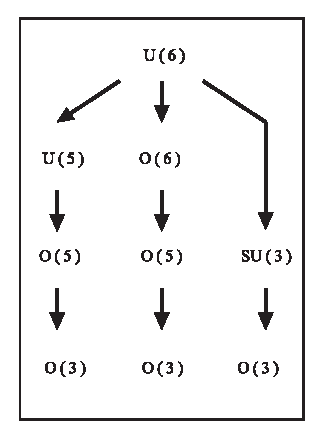
\includegraphics[scale=.65]{figure}
%%
%% If not, use
%%\picplace{5cm}{2cm} % Give the correct figure height and width in cm
%%
%\caption{Please write your figure caption here}
%\label{fig:2}       % Give a unique label
%\end{figure}
%
%\runinhead{Run-in Heading Boldface Version} Use the \LaTeX\ automatism for all your cross-references and citations as has already been described in Sect.~\ref{sec:2}.
%
%\subruninhead{Run-in Heading Boldface and Italic Version} Use the \LaTeX\ automatism for all your cross-refer\-ences and citations as has already been described in Sect.~\ref{sec:2}\index{paragraph}.
%
%\subsubruninhead{Run-in Heading Displayed Version} Use the \LaTeX\ automatism for all your cross-refer\-ences and citations as has already been described in Sect.~\ref{sec:2}\index{paragraph}.
%% Use the \index{} command to code your index words
%%
%% For tables use
%%
%\begin{table}[!t]
%\caption{Please write your table caption here}
%\label{tab:1}       % Give a unique label
%%
%% For LaTeX tables use
%%
%\begin{tabular}{p{2cm}p{2.4cm}p{2cm}p{4.9cm}}
%\hline\noalign{\smallskip}
%Classes & Subclass & Length & Action Mechanism  \\
%\noalign{\smallskip}\svhline\noalign{\smallskip}
%Translation & mRNA$^a$  & 22 (19--25) & Translation repression, mRNA cleavage\\
%Translation & mRNA cleavage & 21 & mRNA cleavage\\
%Translation & mRNA  & 21--22 & mRNA cleavage\\
%Translation & mRNA  & 24--26 & Histone and DNA Modification\\
%\noalign{\smallskip}\hline\noalign{\smallskip}
%\end{tabular}
%$^a$ Table foot note (with superscript)
%\end{table}
%%
%\section{Section Heading}
%\label{sec:3}
%% Always give a unique label
%% and use \ref{<label>} for cross-references
%% and \cite{<label>} for bibliographic references
%% use \sectionmark{}
%% to alter or adjust the section heading in the running head
%Instead of simply listing headings of different levels we recommend to let every heading be followed by at least a short passage of text. Furtheron please use the \LaTeX\ automatism for all your cross-references and citations as has already been described in Sect.~\ref{sec:2}.
%
%Please note that the first line of text that follows a heading is not indented, whereas the first lines of all subsequent paragraphs are.
%
%If you want to list definitions or the like we recommend to use the Springer-enhanced \verb|description| environment -- it will automatically render Springer's preferred layout.
%
%\begin{description}[Type 1]
%\item[Type 1]{That addresses central themes pertainng to migration, health, and disease. In Sect.~\ref{sec:1}, Wilson discusses the role of human migration in infectious disease distributions and patterns.}
%\item[Type 2]{That addresses central themes pertainng to migration, health, and disease. In Sect.~\ref{subsec:2}, Wilson discusses the role of human migration in infectious disease distributions and patterns.}
%\end{description}
%
%\subsection{Subsection Heading} %
%In order to avoid simply listing headings of different levels we recommend to let every heading be followed by at least a short passage of text. Use the \LaTeX\ automatism for all your cross-references and citations citations as has already been described in Sect.~\ref{sec:2}.
%
%Please note that the first line of text that follows a heading is not indented, whereas the first lines of all subsequent paragraphs are.
%
%\begin{svgraybox}
%If you want to emphasize complete paragraphs of texts we recommend to use the newly defined Springer class option \verb|graybox| and the newly defined environment \verb|svgraybox|. This will produce a 15 percent screened box 'behind' your text.
%
%If you want to emphasize complete paragraphs of texts we recommend to use the newly defined Springer class option and environment \verb|svgraybox|. This will produce a 15 percent screened box 'behind' your text.
%\end{svgraybox}
%
%
%\subsubsection{Subsubsection Heading}
%Instead of simply listing headings of different levels we recommend to let every heading be followed by at least a short passage of text. Furtheron please use the \LaTeX\ automatism for all your cross-references and citations as has already been described in Sect.~\ref{sec:2}.
%
%Please note that the first line of text that follows a heading is not indented, whereas the first lines of all subsequent paragraphs are.
%
%\begin{theorem}
%Theorem text goes here.
%\end{theorem}
%%
%% or
%%
%\begin{definition}
%Definition text goes here.
%\end{definition}
%
%\begin{proof}
%%\smartqed
%Proof text goes here.
%%\qed
%\end{proof}
%
%\paragraph{Paragraph Heading} %
%Instead of simply listing headings of different levels we recommend to let every heading be followed by at least a short passage of text. Furtheron please use the \LaTeX\ automatism for all your cross-references and citations as has already been described in Sect.~\ref{sec:2}.
%
%Note that the first line of text that follows a heading is not indented, whereas the first lines of all subsequent paragraphs are.
%%
%% For built-in environments use
%%
%\begin{theorem}
%Theorem text goes here.
%\end{theorem}
%%
%\begin{definition}
%Definition text goes here.
%\end{definition}
%%
%\begin{proof}
%%\smartqed
%Proof text goes here.
%%\qed
%\end{proof}
%%
%%
%\begin{trailer}{Cabeza de remolque}
%If you want to emphasize complete paragraphs of texts in an \verb|Trailer Head| we recommend to
%use  \begin{verbatim}\begin{trailer}{Trailer Head}
%...
%\end{trailer}\end{verbatim}
%\end{trailer}
%%
%\begin{question}{Preguntas}
%If you want to emphasize complete paragraphs of texts in an \verb|Questions| we recommend to
%use  \begin{verbatim}\begin{question}{Questions}
%...
%\end{question}\end{verbatim}
%\end{question}
%%
%%
%\begin{important}{Importante}
%If you want to emphasize complete paragraphs of texts in an \verb|Important| we recommend to
%use  \begin{verbatim}\begin{important}{Important}
%...
%\end{important}\end{verbatim}
%\end{important}
%%
%\clearpage
%\begin{warning}{Atención}
%If you want to emphasize complete paragraphs of texts in an \verb|Attention| we recommend to
%use  \begin{verbatim}\begin{warning}{Attention}
%...
%\end{warning}\end{verbatim}
%\end{warning}
%
%\begin{programcode}{Código de programa}
%If you want to emphasize complete paragraphs of texts in an \verb|Program Code| we recommend to
%use
%
%\verb|\begin{programcode}{Program Code}|
%
%\verb|\begin{verbatim}...\end{verbatim}|
%
%\verb|\end{programcode}|
%
%\end{programcode}
%%
%\begin{tips}{Consejos}
%If you want to emphasize complete paragraphs of texts in an \verb|Tips| we recommend to
%use  \begin{verbatim}\begin{tips}{Tips}
%...
%\end{tips}\end{verbatim}
%\end{tips}
%%
%%
%\begin{overview}{Visión general}
%If you want to emphasize complete paragraphs of texts in an \verb|Overview| we recommend to
%use  \begin{verbatim}\begin{overview}{Overview}
%...
%\end{overview}\end{verbatim}
%\end{overview}
%\clearpage
%\begin{backgroundinformation}{Background Information}
%If you want to emphasize complete paragraphs of texts in an \verb|Background|
%\verb|Information| we recommend to
%use
%
%\verb|\begin{backgroundinformation}{Background Information}|
%
%\verb|...|
%
%\verb|\end{backgroundinformation}|
%\end{backgroundinformation}
%\begin{legaltext}{Legal Text}
%If you want to emphasize complete paragraphs of texts in an \verb|Legal Text| we recommend to
%use  \begin{verbatim}\begin{legaltext}{Legal Text}
%...
%\end{legaltext}\end{verbatim}
%\end{legaltext}
%%
%\begin{acknowledgement}
%If you want to include acknowledgments of assistance and the like at the end of an individual chapter please use the \verb|acknowledgement| environment -- it will automatically render Springer's preferred layout.
%\end{acknowledgement}
%%
%\section*{Apéndice}
%\addcontentsline{toc}{section}{Apéndice}
%%
%When placed at the end of a chapter or contribution (as opposed to at the end of the book), the numbering of tables, figures, and equations in the appendix section continues on from that in the main text. Hence please \textit{do not} use the \verb|appendix| command when writing an appendix at the end of your chapter or contribution. If there is only one the appendix is designated ``Appendix'', or ``Appendix 1'', or ``Appendix 2'', etc. if there is more than one.
%
%\begin{equation}
%a \times b = c
%\end{equation}
%% Problems or Exercises should be sorted chapterwise
%\section*{Problemas}
%\addcontentsline{toc}{section}{Problems}
%%
%% Use the following environment.
%% Don't forget to label each problem;
%% the label is needed for the solutions' environment
%\begin{prob}
%\label{prob1}
%A given problem or Excercise is described here. The
%problem is described here. The problem is described here.
%\end{prob}
%
%\begin{prob}
%\label{prob2}
%\textbf{Problem Heading}\\
%(a) The first part of the problem is described here.\\
%(b) The second part of the problem is described here.
%\end{prob}
\renewcommand{\refname}{Referencias bibliográficas}
\nocite{*}
\bibliographystyle{spmpsci}
{\footnotesize 
	\bibliography{bib}}
%[title={Referencias bibliográficas},heading=bibintoc]}
%\biblstarthook{In view of the parallel print and (chapter-wise) online publication of your book at \url{www.springerlink.com} it has been decided that -- as a genreral rule --  references should be sorted chapter-wise and placed at the end of the individual chapters. However, upon agreement with your contact at Springer you may list your references in a single seperate chapter at the end of your book. Deactivate the class option \texttt{sectrefs} and the \texttt{thebibliography} environment will be put out as a chapter of its own.\\\indent
%References may be \textit{cited} in the text either by number (preferred) or by author/year.\footnote{Make sure that all references from the list are cited in the text. Those not cited should be moved to a separate \textit{Further Reading} section or chapter.} If the citatiion in the text is numbered, the reference list should be arranged in ascending order. If the citation in the text is author/year, the reference list should be \textit{sorted} alphabetically and if there are several works by the same author, the following order should be used:
\endgroup
%%%%%%%%%%%%%%%%%%%%%%%%%%%%%%%%%%%%%%%% Segunda parte %%%%%%%%%%%%%%%%%%%%%%%%%%%%%%%%%%%%%%%%
%\begin{partbacktext}
\part{Realización numérica}
La segunda parte de la monografía se dedica a las realizaciones prácticas de problemas. Combinaremos las consideraciones teóricas sobre diferentes modelos y ecuaciones con las técnicas. Al principio presentamos modelos alternativos para problemas de interacción. En el capítulo $3$ estudiamos la formulación variacional. Este modelo debe ser considerado como la técnica más avanzada. Damos detalles en la construcción de . Segundo, la formulación es introducida en el capítulo $4$. Este nuevo enfoque alternativo es adecuado para problemas con. Nuevamente, presentamos las herramientas necesarias de discretización y simulación. El capítulo $5$ se ocupa de las herramientas para la solución de los problemas algebraicos que surgen de la discretización. En ambos casos, tenemos que lidiar con problemas muy grandes, no lineales. Finalmente, el capítulo $6$ introduce el concepto de tiempo de escala para la reducción de la dimensión de los esquemas discretos que nos permitirá reducir significativamente la complejidad de los sistemas.
\end{partbacktext}
%\chapauthor{Autor}
%\chapsubtitle{Subtítulo}
\chapter{Método de Euler}\index{Método de Euler}
\abstract{En este capítulo introducimos un tipo de funciones llamadas que pueden ser usados para aproximar otras funciones más generales}
%\chaptermark{xd}
\section{Ecuación diferencial ordinaria lineal}
\begingroup
\let\clearpage\relax
%%\chapauthor{Autor}
%\chapsubtitle{Subtítulo}
\chapter{Método de Euler}\index{Método de Euler}
\abstract{En este capítulo introducimos un tipo de funciones llamadas que pueden ser usados para aproximar otras funciones más generales}
%\chaptermark{xd}
\section{Ecuación diferencial ordinaria lineal}
Una aplicación inmediata del método de las diferencias finitas para aproximar derivada es la solución aproximada de los problemas de valor inicial para ecuaciones diferenciales ordinarias. El uso de la forma general de tal problema es
\begin{equation}\label{eq:ivp}
y^{\prime}=f\left[t,y\right],\quad y\left(t_{0}\right)=y_{0},
\end{equation}
donde $f$ es la función desconocida de $t$ e $y$, y $t_{0}$ y $y_{0}$ son los valores dados. El objetivo en la solución de este problema es encontrar la función $y$ como una función de $t$, en el curso usual en ecuaciones diferenciales ordinarias, el estudiante aprende un número de técnicas para resolver analíticamente~\eqref{eq:ivp}, basado sobre la asunción de cualquier número de formas especiales para $f$. Aquí usaremos una de nuestras aproximaciones de la derivada para construir un método para aproximadamente resolver ~\eqref{eq:ivp}.

Usamos %
para remplazar la derivada en~\eqref{eq:ivp}:
\begin{align*}
\frac{y\left(t+h\right)-y\left(t\right)}{h}
&=f\left(t,y\left(t\right)\right)+\frac{1}{2}hy^{\prime\prime}\left(t_{h}\right),
\shortintertext{el cual puede ser simplificado cuidadosamente hasta}% TODO:
y\left(t+h\right)&=y\left(t\right)+hf\left(t,y\left(t\right)\right)+\frac{1}{2}h^{2}y^{\prime\prime}\left(t_{h}\right).
\end{align*}
Esto sugire el siguiente método numérico:
\begin{enumerate}
	\item Defina una sucesión de $t$ valores (llamado una \emph{malla}) de acuerdo con $t_{n}=t_{0}+nh$, donde $h$ es el parámetro fijado (llamado el \emph{espacio de la malla} o \emph{tamaño de la grilla}), encontraremos este tipo de cosa con frecuencia en tópicos posteriores.
	\item Calcule los valores $y_{n}$ a partir de $y_{0}$ y los $t$ valores de la malla %TODO
	, de acuerdo con
	\begin{equation}\label{eq:euler}
	y_{n+1}=y_{n}+hf\left(t_{n},y_{n}\right).
	\end{equation}
\end{enumerate}
Note que esto se sigue de%
por %
el término de error y ajustando la notación cuidadosamente.

La ecuación~\eqref{eq:euler} define lo que es conocido como el \emph{método de Euler} para resolver (aproximadamente) los problemas de valor inicial para ecuaciones diferenciales ordinarias. La figura X muestra qué está ocurriendo geométricamente.

\begin{example}
	Considere el problema de valor inicial \[ y^{\prime}=-y+\sin t,\quad y\left(0\right)=1. \]
	Este tiene exactamente la solución $y\left(t\right)=\frac{3}{2}e^{-t}+\frac{1}{2}\left(\sin t-\cos t\right)$, encontrado al usar los tipos de métodos enseñados en un curso usual de EDO. Si aplicamos el método de Euler para esto, usando $h=\frac{1}{4}$, obtenemos los siguientes resultados.
	\begin{enumerate}[Paso 1]
		\item Tenemos $h=\frac{1}{4}$, así $t_{1}=h=\frac{1}{4}$ y $y_{0}$ es dado como $1$. Entonces, \[ y_{1}=y_{0}+hf\left(t_{0},y_{0}\right)=1+\frac{1}{4}\left(-1+\sin 0\right)=\frac{3}{4}. \] Así, y$\left(1/4\right)\approx0.75$, y el error en esta aproximación es $e_{1}=y\left(1/4\right)-y_{1}=0.8074469434-0.75=0.0574469434$.
		\item Tenemos $t_{2}=2h=\frac{1}{2}$ y $y_{1}=0.75$ del paso 1%
		Entonces, \[ y_{2}=y_{1}+hf\left(t_{1},y_{1}\right)=\frac{3}{4}+\frac{1}{4}\left(-\frac{3}{4}+\sin\frac{1}{4}\right)=0.6243509898. \] Así, $y\left[1/2\right]-y_{2}=0.710774779-0.6242509898=0.0863664881$.
	\end{enumerate}
\end{example}\footnote{Leonhard Euler (1707--1783) fue uno de los grandes matemáticos de la era pos Newton, el otro fue Carl Friedrich Gauß. Euler nació en Basilea, Suiza, y se educó en la Universidad de Basilea, el primero con un ojo siguiendo en la carrera de su padre como ministro Luterano. Con la asistencia de su tutor y su mentor Johann Bernoulli, sin embargo, él fue capaz de convencer a su pare a perseguir una carrera de matemáticas. En 1727, Euler ingresó a la Academia de Ciencias de San Petersburgo en Rusia, donde él estuvo hasta 1741, en su tiempo ĺe ingreso a la Academia de Ciencias de Berlín por la invitación del rey de Prusia, Federico el grande. Después de algunas disputas con el monarca, Euler dejó Berlín en 1766 y regresó a San Petersburgo. Las contribuciones de Euler a las matemáticas son %
Él publicó una enorme cantidad de material, en una amplia variedad de áreas, incluyendo series infinitas, funciones especiales (un campo de estudio que él prácticamente inventó), teoría de números, variables complejas e hidrodinámicas. Su nombre es adjuntado a resultados%
en matemáticas, desde la fórmula de Euler que relaciona las funciones trigonométricas para la exponencial compleja, hasta las ecuaciones diferenciales de Euler-Cauchy, hasta la fórmula de Euler que relaciona el número de caras, aristas y vértices en un poliedro. Su influencia en la notación se siente hasta el día de hoy por el uso de $\Sigma$ para denotar sumas, $\cos y $$\sin$ para el coseno y seno de un ángulo. Los trabajos recolectados de Euler, publicado entre 1911 y 1975 alcanza los 72 volúmenes!

El método para resolver numéricamente ecuaciones diferenciales que lleva su nombre fue aparentemente presentado en el periodo 1768--1769, en los volúmenes de su trabajo \emph{Institutionum calculi integralis}. La base teórica para la convergencia de este método fue %
por Augustin Louis Cauchy en los mediados de 1800 y por Rudolf Lipschitz en los finales de 1800.
}

Si en vez de usar $h=\frac{1}{8}$ y continuar el cálculo para $t=1$, entonces mostramos la tabla.

Si dividimos el tamaño de la malla en la mitad, nuevamente, para $h=\frac{1}{16}$, entonces obtenemos los resultados en la Tabla X. Note que para $h=\frac{1}{8}$, el error máximo es dado por $4.425\times 10^{-2}$, donde $h=\frac{1}{16}$ este es dado por $2.140\times10^{-2}$. Esto sugiere (pero no prueba) que el método de Euler es $\mathcal{O}\left(h\right)$ preciso, algo que probaremos en \autoref{ch:6}, donde tomamos un rango más amplio de estudio de los métodos numéricos para ecuaciones diferenciales. Esto es adecuado, pero no preciso %
preferimos un método que sea $\mathcal{O}\left(h^{p}\right)$ preciso para $p\geq2.$

La figura X muestra la solución exacta (línea sólida), la solución aproximada calculado con $h=\frac{1}{8}$ (denotada por asteriscos), y la solución aproximada calculada con $h=\frac{1}{16}$ (denotada por los signos más). Note que los signos más (aquellos valores calculados con una malla menor) aparece ser más precioso.

Escribiendo el código de computadora para el método de Euler no es difícil. Si asumimos que $h$, el tamaño de la malla, es dado, junto con $N$, el número de pasos a tomar, entonces el código luciría algo como el código dado en el algoritmo X

\newpage

Ahora nos concentraremos aquí con el problema de resolver ecuaciones diferenciales. numéricamente. Primero, nos concentramos en el llamado \emph{problema de valor inicial} (PVI): Encuentre una función $y\left(t\right)$ tal que \[ \frac{dy}{dt}=f\left(t,y\left(t\right)\right),\quad y\left(t_{0}\right)=y_{0}, \] donde $f$ es una función desconocida de dos variables, $t_{0}$ y $y_{0}$ son valores conocidos. Este es llamado el problema de valor inicial porque (como la notación sugiere) podemos ver el término independiente $t$ como el tiempo, y la ecuación como el modelamiento de un proceso que mueve anteriormente desde algún tiempo inicial $t_{0}$ con estado inicial $y_{0}$. (Muy frecuentemente, $t_{0}=0$.) La variable dependiente $y$, la función desconocida, podría ser una función escalar o, posiblemente, una función vectorial definida como \[ y\left(t\right)={\left(y_{1}\left(t\right),y_{2}\left(t\right)\ldots,y_{N}\left(t\right)\right)}^{T}. \] En \ref{} desarrollamos el método de Euler para aproximar soluciones de problemas de valor inicial. En este capítulo no solo revisaremos el método de Euler, sino también veremos métodos más sofisticados (y por lo tanto, esperamos más preciso) para resolver este tipo de problemas. Más adelante, atacaremos los problemas de valor de frontera, que puede ser escrito como
\begin{align*}
-\frac{d^{2}u}{dx^{2}}&=F\left(x,u,\frac{du}{dx}\right),\quad a<x<b,\\
u\left(a\right)&=g_{0},\\
u\left(b\right)&=g_{1}.
\end{align*}
Aquí la función desconocida es $u$ con variable independiente $x$, $F$ es una función desconocida de tres variables, y $g_{0}$ y $g$ son los datos iniciales conocidos. Muy frecuentemente el intervalo $\left(a,b\right)=\left(0,1\right)$.

En ambos casos queremos encontrar una función desconocida. Haremos esto aproximando los puntos individuales en la gráfica de la función. así como lo hicimos en \ref{} con el método de Euler para los problemas de valor inicial. Por lo tanto, esperaremos (en el caso del PVI) un conjunto de valores $y_{k}$ tal que $y_{k}\approx y\left(t_{k}\right)$ para algún conjunto de puntos en la grilla $t_{k}$ (conocido), o (en el caso del PVF) un conjunto de valores $u_{k}$ tal que $u_{k}\approx u\left(u_{k}\right)$ para algún conjunto de puntos en la grilla (conocido) $x_{k}$. Note que esto significa que nuestra aproximación es solo definida en los puntos de la grilla, a menos podríamos usar los métodos de la aproximación del %\autoref{}
 para construir soluciones que aproximen continuamente a las ecuaciones diferenciales, esto es algo que es frecuentemente hecho, y mostramos un ejemplo de este, donde usamos esplines para resolver problemas con dos valores de frontera.
 
En X, %
introducimos el método de los elementos finitos para PVF, el cual también usa la noción de expandir la aproximación como una combinación lineal de funciones simples. 

En el %\autoref{}
revisamos esta idea (y extendemos esto para algunas ecuaciones en derivadas parciales EDP). Pero en este capítulo nos concentraremos en lo básico.

Debería notarse que la solución numérica de las ecuaciones diferenciales ordinarias (tanto los PVI o los PVF), es un área de investigación con mucha actividad. El lector es invitado a revisar la lista de referencias en el fin de este capítulo para un tratamiento más profundo de este material.

\section{El problema de valor inicial}
Considere la ecuación diferencial ordinaria
\begin{equation}\label{eq:ode}
\frac{dy}{dt}=f\left(t,y\left(t\right)\right),\quad y\left(t_{0}\right)=y_{0},
\end{equation}
 donde $f$ es una función desde $\mathds{R}^{N+1}$ en $\mathds{R}^{N}$ para algún  $N>0$ (si $N>1$, entonces tenemos una ecuación escalar, caso contrario, una ecuación vectorial), $t_{0}$ es un valor escalar dado, frecuentemente tomado como $t_{0}=0$, y conocido como el \emph{punto inicial} e $y_{0}$ es conocido como el vector en $\mathds{R}^{N}$, conocido como el \emph{valor inicial}. Queremos encontrar la función desconocida $y\left(t\right)$, el cuál resuelve~\eqref{eq:ode} en el sentido que \[ y^{\prime}\left(t\right)-f\left(t,y\left(t\right)\right)=0 \] para todo $t>t_{0}$, e $y\left(t_{0}\right)=y_{0}$.
 
\begin{example}
	Considere el problema \[ y^{\prime}=-2ty,\quad y\left(0\right)=1. \]
\end{example}
Aquí $f\left(t,y\right)$
%%%%%%%%%%%%%%%%%%%%
\newpage

Las ecuaciones diferenciales surgen cuando tenemos información sobre la tasa de cambio de una cantidad, en lugar de la cantidad en sí.

Por ejemplo, sabemos que la tasa de descomposición de una sustancia radiactiva es proporcional a la masa $m$ de la sustancia remanente en el tiempo $t$. Podemos escribir esto como una ecuación diferencial:
\[ \frac{dm}{dt}=-km \]
donde $k$ es una constante. Lo que realmente nos gustaría es una expresión para la masa $m$ en el tiempo $t$. Usando las técnicas desarrolladas en este capítulo, encontraremos que la solución general a esta ecuación diferencial es $m=Ae^{-kt}$.

Las ecuaciones diferenciales tienen muchas aplicaciones en la ciencia, ingeniería y economía, y su estudio es una rama importante de las matemáticas. Para matemáticas Especializadas, consideramos solo una variedad limitada de ecuaciones diferenciales.

\section{Una introducción a las ecuaciones diferenciales}

Una ecuación diferencial contiene derivadas de una función o variable particular. Los siguientes son ejemplos de ecuaciones diferenciales:
\[ \frac{dy}{dx}=\cos x,\quad\frac{d^{2}y}{dx^{2}}-4\frac{dy}{dx}=0,\quad\frac{dy}{dx}=\frac{y}{y+1} \]

La solución de una ecuación diferencial es una definición clara de la función o relación, sin ninguna de sus derivadas involucradas.

Por ejemplo, si $\frac{dy}{dx}=\cos x$, entonces $y=\int\cos x\mathrm{d}x$ y así, $y=\sin x+c$.

Aquí $y=\sin x+c$ es la \textbf{solución general} de la ecuación diferencial $\frac{dy}{dx}=\cos x$.

Este ejemplo muestra las características principales de tales soluciones. Las soluciones de ecuaciones diferenciales son el resultado de una integral, y por lo tanto producen una familia de funciones.

Para obtener una \textbf{solución particular}, requerimos información adicional, que generalmente se proporciona como un par ordenado que pertenece a la función o relación. (Para las ecuaciones con segundas derivadas, necesitamos dos elementos de información).

\subsection{Verificando una solución de una ecuación diferencial}

Podemos verificar que una expresión particular es una solución de una ecuación diferencial por sustitución. Esto se demuestra en los siguientes ejemplos.

Usaremos la siguiente notación para indicar el valor de $y$ para un valor de $x$ dado:
\[ y(0)=3 \text{ significará que cuando }x = 0, y = 3. \]
Consideramos $y$ como una función de $x$. Esta notación es útil en ecuaciones diferenciales.

\begin{example}
	\begin{enumerate}
		\item Verifique que $y=Ae^{x}-x-1$ es una solución de la ecuación diferencial $\frac{dy}{dx}=x+y$.
		\item Por lo tanto, encuentre la solución particular de la ecuación diferencial dado que $y(0)=3$.
	\end{enumerate}
\end{example}

\begin{enumerate}
	\item Sea $y=Ae^{x}-x-1$. Necesitamos verificar que $\frac{dy}{dx}=x+y$.
	\begin{align*}
	\text{LHS}
	&=\frac{dy}{dx}\\
	&=Ae^{x}-1\\
	\text{RHS}
	&=x+y\\
	&=x+Ae^{x}-x-1\\
	&=Ae^{x}-1
	\end{align*}
	Por lo tanto $\text{LHS}=\text{RHS}$ y así $y=Ae^{x}-x-1$ es una solución de $\frac{dy}{dx}=x+y$.
	\item $y\left(0\right)=3$ significa $y\left(0\right)=3$ significa que cuando $x=0$, $y=3$. Sustituyendo en la solución $y=Ae^{x}-x-1$  verificado en a:% TODO:
	\begin{align*}
	3&=Ae^{0}-0-1\\
	3&=A-1\\
	\therefore\quad A&=4.
	\end{align*}
	La solución particular es $y=4e^{x}-x-1$.
	3 = Ae0 - 0 - 1
	3 = A - 1
	∴
	A = 4
	La solución particular es y = 4e x - x - 1.
\end{enumerate}


\begin{example}
	Verifique que $y=e^{2x}$ es una solución de la ecuación diferencial $\frac{d^{2}y}{dx^{2}}+\frac{dy}{dx}-6y=0$.
\end{example}

Sea $y=e^{2x}$, entonces $\frac{dy}{dx}=2e^{2x}$ y $\frac{d^{2}y}{dx^{2}}=3e^{2x}$. Ahora considere la ecuación diferencial:
\begin{align*}
\text{LHS}
&=\frac{d^{2}y}{dx^{2}}+\frac{dy}{dx}-6y\\
&=4e^{2x}+2e^{2x}-6e^{2x}\quad(\text{de ariiba})\\
&=0\\
&=\text{RHS}.
\end{align*}

\begin{example}
	Verigique que $y=ae^{2x}+be^{-3x}$ es una solución de la ecuación diferencial $\frac{d^{2}y}{dx^{2}}+\frac{dy}{dx}-6y=0$.
\end{example}

Sea $y=ae^{2x}+be^{-3x}$, entonces $\frac{dy}{dx}=2ae^{2x}-3be^{-3x}$ y $\frac{d^{2}y}{dx^{2}}=4ae^{2x}+9be^{-3x}$. Así,
\begin{align*}
	\text{LHS}
	&=\frac{d^{2}y}{dx^{2}}+\frac{dy}{dx}-6y\\
	&=\left(4ae^{2x}+9be^{-3x}\right)+\left(2ae^{2x}-3be^{-3x}\right)-6\left(ae^{2x}+be^{-3x}\right)\\
	&=4ae^{2x}+9be^{-3x}+2ae^{2x}-3be^{-3x}-6ae^{2x}-6be^{-3x}\\
	&=0\\
	&=\text{RHS}.
\end{align*}

\begin{example}
	Encuentre las constantes $a$ y $b$ si $y=e^{4x}\left(2x+1\right)$ es una solución de la ecuación diferencial \[ \frac{d^{2}y}{dx^{2}}-a\frac{dy}{dx}+by=0. \]
\end{example}

Sea $y=e^{4x}\left(2x+1\right)$, entonces
\begin{align*}
\frac{dy}{dx}
&=4e^{4x}\left(2x+1\right)+2e^{4x}\\
&=2e^{4x}\left(4x+2+1\right)\\
&=2e^{4x}\left(4x+3\right)
\shortintertext{y}
\frac{d^{2}y}{dx^{2}}
&=8e^{4x}\left(4x+3\right)+4\times2e^{4x}\\
&=8e^{4x}\left(4x+3+1\right)\\
&=8e^{4x}\left(4x+4\right)\\
&=32e^{4x}\left(x+1\right).
\end{align*}

Si $y=e^{4x}\left(2x+1\right)$ es una solución de la ecuación diferencial, entonces
\[ \frac{d^{2}y}{dx^{2}}-a\frac{dy}{dx}+by=0, \]
es decir, $32e^{4x}\left(x+1\right)-2ae^{4x}\left(4x+3\right)+be^{4x}\left(2x+1\right)=0$. Podemos dividir por $e^{4x}$ (ya que $e^{4x}>0$):
\begin{align*}
32x+32-8ax-6a+2bx+b&=0
\shortintertext{es decir,}
\left(32-8a+2b\right)x+\left(32-6a+b\right)&=0
\end{align*}
Por lo tanto,
\begin{align}
32-8a+2b	&=0 \label{eq:1}\\
32-6a+b		&=0 \label{eq:2}\\
\end{align}
Multiplicando~\eqref{eq:2} por $2$ y restando~\eqref{eq:1}: \[ -32+4a=0. \] Así, $a=8$ y $b=16$.

\section{Ecuaciones diferenciales}

Estas ecuaciones diferenciales son similares a las discutidas anteriormente, con la antidiferenciación siendo aplicado dos veces.

Sea $p=\frac{dy}{dx}$, entonces $\frac{d^{2}y}{dx^{2}x}=\frac{dp}{dx}=f\left(x\right)$. La técnica consiste en encontrar primero $p$ como la solución de la ecuación diferencial $\frac{dp}{dx}=f\left(x\right)$ y luego sustituyendo $p$ en $\frac{dy}{dx}=p$ y resolviendo esta ecuación diferencial.

\begin{example}
\end{example}

En esta sección discutimos un método para encontrar una solución aproximada a una ecuación diferencial. Esto se logra encontrando una sucesión finita de puntos $(x_{0},y_{0}),(x_{1},y_{1}),(x_{2},y_{2}),\ldots,(x_{n},y_{n})$ que se encuentran en una curva que se aproxima a la curva de solución de la ecuación diferencial dada.

\subsection{Aproximación lineal a la curva}
Para el diagrama, tenemos \[ \frac{f\left(x+h\right)-f\left(x\right)}{h}\approx f^{\prime}\left(x\right)\text{ para un pequeño }h \] Reordenando esta ecuación da \[ f\left(x+h\right)\approx f\left(x\right)+hf^{\prime}\left(x\right). \]
Esto se muestra en el diagrama. La recta $\ell$ es tangente a $y=f(x)$ en el punto con coordenadas $(x,f(x))$.

Esto da una aproximación a la curva $y=f(x)$ en que la coordenada $y$ de $B$ es una
aproximación a la coordenada $y$ de $A$ en la gráfica de $y=f(x)$.
\subsection{El proceso general}
Este proceso se puede repetir para generar un sucesión de puntos más larga.


Comenzamos de nuevo del principio. Considere la ecuación diferencial
\[ \frac{dy}{dx}=g\left(x\right)\quad\text{con}\quad y\left(x_{0}\right)=y_{0}. \]
Entonces $x_{1}=x_{0}+h$ y e1 $y_{1}=y_{0}+hg(x0)$.

El proceso ahora se aplica repetidamente para aproximar el valor de la función en $x_{2},x_{3},\ldots$.

El resultado es:
\begin{align*}
x_{2}=x_{1}+h\quad\text{y}\quad y_{2}=y_{1}+hg(x_{1})\\
x_{3}=x_{2}+h\quad\text{y}\quad y_{3}=y_{2}+hg(x_{2})
\end{align*}
y así.

El punto $\left(x_{n},y_{n}\right)$ se encuentra en el $n$--ésimo paso del proceso iterativo.

Este proceso iterativo se puede resumir de la siguiente manera.

\begin{theorem}[Método de Euler]
	Si $\frac{dy}{dx}=g\left(x\right)$ con $x_{0}=a$ e $y_{0}=b$, entonces $x_{n+1}=x_{n}+h$ e $y_{n+1}=y_{n}+hg\left(x_{n}\right)$.
\end{theorem}

La precisión de esta fórmula, y el proceso asociado, se puede comparar con los valores
Obtenido a través de la solución de la ecuación diferencial, donde se conoce el resultado.

\section{Variantes del método de Euler}

El método de Euler, por supuesto, no es el único ni el mejor esquema para aproximar soluciones a problemas de valor inicial, y lo que debemos hacer ahora es buscar otros métodos que podamos emplear. Varias ideas pueden ser consideradas basadas en algunas extensiones simples de una derivación del método de Euler.

Nuestra tercera derivación del método de Euler, que también nos da un término restante, se basa en nuestros métodos de diferencia para la aproximación derivada %(de §2.2).

Comenzamos con la ecuación diferencial
\[ y^{\prime}\left(t\right)=f\left(t,y\left(t\right)\right) \]
y reemplace la derivada con y reemplace la derivada con el cociente de diferencia simple derivado en %(2.1).
Esto resulta
\[ \frac{y\left(t+h\right)-y\left(t\right)}{h}=f\left(t,y\left(t\right)\right)+\frac{1}{2}hy^{\prime\prime}\left(\theta_{t,h}\right) \]
donde los subíndices en $\theta$ nos recuerdan que el valor depende tanto de $t$ como de $h$. El método de Euler es entonces obtenido simplemente dejando caer el resto, y reemplazando $t$ por $t_{n}$ y $y\left(t\right)$ con $y_{n}$, y así sucesivamente. Esta es la derivación que usamos en el %Capítulo 2.

Esto plantea una pregunta obvia: ?`Qué sucede si utilizamos otras aproximaciones a la
derivada? Por ejemplo, si usamos
\[ y^{\prime}\left(t\right)=\frac{y\left(t\right)-y\left(t-h\right)}{h}-\frac{1}{2}hy^{\prime\prime}\left(\theta\right), \]
entonces obtenemos el método de Euler hacia atrás:
\begin{equation}
y_{n+1}=y_{n}+hf\left(t_{n+1},y_{n+1}\right),
\end{equation}
y si usamos
\[ y^{\prime}\left(t\right)=\frac{y\left(t+h\right)-y\left(t-h\right)}{2h}-\frac{1}{6}h^{2}y^{\prime\prime\prime}\left(\theta_{t,h}\right) \]
obtenemos lo que comúnmente se conoce como el método del punto medio:
\[ y_{n+1}=y_{n-1}+2hf\left(t_{n},y_{n}\right). \]
O, podríamos usar las aproximaciones derivadas basadas en la interpolación %(§4.5):
\begin{align*}
y^{\prime}\left(t\right)\approx\frac{1}{2h}\left(-y\left(t+2h\right)+4y\left(t+h\right)-3y\left(t\right)\right),\\
y^{\prime}\left(t+2h\right)\approx\frac{1}{2h}\left(3y\left(t+2h\right)-4y\left(t+h\right)+y\left(t\right)\right),
\end{align*}
para obtener los dos métodos numéricos
\begin{align*}
	y_{n+1}&=4y_{n}-3y_{n-1}-2hf\left(t_{n-1},y_{n-1}\right),
	\shortintertext{y}
	y_{n+1}&=\frac{4}{3}y_{n}-\frac{1}{3}y_{n-1}+\frac{2}{3}hf\left(t_{n+1},y_{n+1}\right).
\end{align*}

Finalmente, observamos que se puede derivar otro conjunto de métodos integrando la ecuación diferencial. Tenemos que la solución exacta satisface
\begin{equation}\label{eq:combeuler}
y\left(t+h\right)=y\left(t\right)+\int_{t}^{t+h}f\left(s,y\left(s\right)\right)\mathrm{d}s.
\end{equation}
Por lo tanto, podemos aplicar la regla del trapecio a~\eqref{eq:combeuler} para  obtener
\begin{equation}\label{eq:combeulerb}
y\left(t+h\right)=y\left(t\right)+\frac{1}{2}h\left[f\left(t+h,y\left(t+h\right)\right)+f\left(t,y\left(t\right)\right)\right]-\frac{1}{2}h^{3}y^{\prime\prime\prime}\left(\theta_{t,h}\right).
\end{equation}
donde $\theta_{t,h}\in\left[t,t+h\right]$ y recordamos al lector que
\[ f\left(t,y\left(t\right)\right)=y^{\prime}\left(t\right)\implies\frac{d^{2}}{dt^{2}}f\left(t,y\left(t\right)\right)=y^{\prime\prime\prime}\left(t\right). \]
Eliminar el resto de~\eqref{eq:combeulerb} conduce al método numérico (comúnmente llamado método trapezoidal, por obvias razones)
\begin{equation}
y_{n+1}=y_{n}+\frac{1}{2}hf\left(f\left(t_{n+1},y_{n+1}\right)+f\left(t_{n},y_{n}\right)\right)
\end{equation}
Alternativamente, podemos usar una aproximación de regla de punto medio para la integración~\eqref{eq:combeuler}. Esto lleva a
\[ y\left(t+h\right)=y\left(t\right)+hf\left(t+\frac{1}{2}h,y\left(t+\frac{1}{2}h\right)\right)-\frac{1}{24}h^{3}y^{\prime\prime\prime}\left(\theta_{t,h}\right), \]
lo que sugiere el método numérico
\begin{equation}
y_{n+1}=y_{n}+hf\left(t_{n+1/2},y_{n+1/2}\right),
\end{equation}
donde $t_{n+1/2}=t_{n}+\frac{1}{2}h$ y $y_{n+1/2}\approx y\left(t_{n}+\frac{1}{2}h\right)$. Esto es similar a %X

?`Qué pasa con estos métodos? ?`Alguno de ellos es bueno?

Varias observaciones se pueden hacer de inmediato. Los métodos (6.21), (6.22) y (6.23)
todas se basan en aproximaciones derivadas que son $\mathcal{O}\left(h^{2}\right)$, mientras que el método de Euler fue basado en una aproximación derivada que es solo $\mathcal{O}\left(h\right)$ (como lo es el método de Euler hacia atrás) (6.20)). Esto nos sugiere (pero no prueba, por supuesto) que (6.21), (6.22) y (6.23)
debería ser más preciso que Euler (y Euler hacia atrás). Del mismo modo, los métodos (6.26) y (6.27) se basan en aproximaciones integrales que son más precisas.

Una segunda observación involucra el método del punto medio (6.21) y los dos métodos (6.22) y (6.23). Tenga en cuenta que aquí tenemos fórmulas para $y_{n+1}$ en términos de $y_{n}$ $y_{n-1}$. Estos no son métodos de un \emph{solo paso}, son métodos de \emph{varios pasos}, es decir, dependen de la información de más de un valor aproximado anterior de la función desconocida. ?`Cómo podemos en realidad implementar estos métodos? La ecuación diferencial solo nos da un único valor inicial, $y_{0}$, necesitamos más para comenzar la recursión aquí.


Una tercera observación se refiere al método de Euler posterior y los métodos (6.26) y (6.23). Note que todas estas fórmulas involucran $f\left(t_{n+1},y_{n+1}\right)$. No podemos resolver explícitamente para el nuevo valor aproximado $y_{n+1}$, por lo que estos métodos (y otros similares) se llaman \emph{implícitos}, mientras que los métodos como Euler, punto medio y (6.22) se llaman \emph{explícitos}, porque define $y_{n+1}$ explícitamente en términos de información de los pasos anteriores.


Nos gustaría abordar el tema de la precisión, al menos de manera experimental, pero no podemos incluso implementar varios de los métodos hasta que abordemos los otros problemas. De todos modos, eso será útil, en este punto, para introducir alguna terminología asociada con la precisión de Los diversos métodos.

\begin{definition}[Orden de precisión]
Si el error de truncamiento para un esquema numérico para la solución de problemas de valor inicial es $\mathcal{O}\left(h^{k}\right)$, entonces decimos que el método tiene un \emph{orden de precisión} $k$.
\end{definition}


\section{Métodos de un solo paso: Runge--Kutta}
La familia de métodos Runge-Kutta\footnote{Martín Wilhelm Kutta (1867--1944) estudió en Breslavia y Múnich, además de un año pasado en Gran Bretaña en Cambridge. La mayor parte de su carrera profesional la pasó en Stuttgart. Sobre la base de la idea original de Runge (primera vez presentado en un artículo de 1894), Kutta publicó su versión de los métodos Runge-Kutta en 1901.} es una de las familias más populares de solucionadores precisos para problemas de valor inicial. La derivación general puede llegar a ser muy complicada; Para evitar el ahogamiento en un mar de detalles y notaciones, resumiremos las ideas básicas utilizando el caso de segundo orden. Recuerde la formulación habitual de predictor-corrector del método trapezoidal:
\begin{align*}
\tilde{y}_{n+1}
&=y_{n}+hf\left(t_{n},y_{n}\right),\\
y_{n+1}
&=y_{n}+\frac{1}{2}h\left[f\left(t_{n+1},\tilde{y}_{n+1}\right)+f\left(t_{n},y_{n}\right)\right].
\end{align*}
Podemos sustituir directamente el predictor en el corrector para escribir esto como una sola recursión:
\begin{equation}\label{eq:dedrunge}
y_{n+1}=
y_{n}+\frac{1}{2}h\left[f\left(t_{n+1},y_{n}+hf\left(t_{n},y_{n}\right)\right)+f\left(t_{n},y_{n}\right)\right]
\end{equation}
Dado que la ecuación diferencial implica que $f$ da valores de $y^{\prime}$, se sigue que podemos ver~\eqref{eq:dedrunge} como definiendo $y_{n+1}$ de $y_{n}$ avanzando a lo largo de una línea recta definida por el simple promedio de las dos pendientes $f\left(t_{n},y_{n}\right)$ y $f\left(t_{n+1},\overline{y}\right)$, donde $\overline{y}=y_{n}+hf\left(t_{n},y_{n}\right)$. Esta plantea la pregunta, por supuesto, de si un promedio diferente de dos pendientes podría o no producir un método más preciso. Para ello, consideramos el método más general.
\begin{equation}\label{eq:casirunge}
y_{n+1}=y_{n}+c_{1}hf\left(t_{n},y_{n}\right)+c_{2}hf\left(t_{n}+\alpha h, y_{n}+\beta hf\left(t_{n},y_{n}\right)\right),
\end{equation}
donde $c_{1}$, $c_{2}$, $\alpha$, $\beta$ son parámetros aún no determinados. Queremos elegir estos para que la solución aproximada definida por~\eqref{eq:dedrunge} es lo más precisa posible y queremos hacer
el error de truncamiento lo más pequeño posible, en términos de potencias de $h$. Por lo tanto, nos fijamos en la expresión
\begin{equation}
R=y\left(t+h\right)-y\left(t\right)-c_{1}hf\left(t,y\left(t\right)\right)-c_{2}hf\left(t+\alpha h, y\left(t\right)\right)+\beta hf\left(t,y\left(t\right)\right).
\end{equation}
Para reducir esto de modo que podamos inferir los valores correctos de $c_{1}$, $c_{2}$, $\alpha$ y $\beta$ que darán como resultado el residual más pequeña $R$, tendremos que usar el teorema de Taylor en dos variables, que indicamos aquí sin demostración:
\begin{align*}
F\left(x+h,y+\eta\right)
&=F\left(x,y\right)+hF_{x}\left(x,y\right)+\eta F_{y}\left(x,y\right)+\frac{1}{2}\left(h^{2}F_{xx}\left(x,y\right)\right)\\
&+h\eta F_{xy}\left(x,y\right)+\eta^{2}F_{yy}\left(x,y\right)+\mathcal{O}\left(h^{3}+\eta^{3}\right).
\end{align*}

\newpage

\section{Análisis del método de Euler}
En esta sección probaremos dos resultados que establecen la convergencia y la estimación de error para el método de Euler. En esta sección proporcionamos una gran cantidad de detalles para evitar entrar en tantos detalles con métodos más sofisticados que se derivarán más adelante. A lo largo de la sección nos ocupamos de la solución aproximada, a través del método de Euler, del problema del valor inicial
\[ y^{\prime}=f\left(t,y\right),\quad y\left(t_{0}\right)=y_{0}. \]
El primer teorema muestra que el método de Euler es, de hecho, de primer orden preciso.

\begin{theorem}[Estimación del error del método de Euler]
Sea $f$ Lipschitz continua, con coeficiente $K$, y asuma que la solución $y\in C^{2}\left(\left[t_{0},T\right]\right)$ para algún $T>t_{0}$. Entonces
\[ \max_{t_{k}\leq T}\left|y\left(t_{k}\right)-y_{k}\right|\leq C_{0}\left|y\left(t_{0}\right)-y_{0}\right|+Ch\|y^{\prime\prime}\|_{\infty,\left[t_{0},T\right]}, \] donde \[ C_{0}=e^{K\left(T-t_{0}\right)} \] y \[ C=\frac{e^{K\left(t-t_{0}\right)-1}}{2K}. \]
\end{theorem}

\begin{proof}
El elemento clave en la prueba de este resultado es el hecho de que la solución exacta satisface la misma relación que la solución aproximada, excepto por la adición de un término restante. Así tenemos (de (6.13) y (6.14)),
\begin{align*}
y\left(t_{n+1}\right)&=y\left(t_{n}\right)+hf\left(t_{n},y\left(t_{n}\right)\right)+\frac{1}{2}h^{2}y^{\prime\prime}\left(\theta_{n}\right),\\
y_{n+1}&=y_{n}+hf\left(t_{n},y_{n}\right),
\end{align*}
que restamos para obtener
\[ y\left(t_{n+1}\right)-y_{n+1}=y\left(t_{n}\right)-y_{n}+hf\left(t_{n},y\left(t_{n}\right)\right)-hf\left(t_{n},y_{n}\right)+\frac{1}{2}h^{2}y^{\prime\prime}\left(\theta_{n}\right). \]
Tome valores absolutos y aplique la continuidad de Lipschitz de $ f$ para obtener
\[ \left|y\left(t_{n+1}\right)-y_{n+1}\right|\leq\left|y\left(t_{n}-y_{n}\right)\right|+Kh\left|y\left(t_{n}\right)-y_{n}\right|+\frac{1}{2}h^{2}\left|y^{\prime\prime}\left(\theta_{n}\right)\right|, \]
que escribimos como
\[ e_{n+1}\leq\gamma e_{n}+R_{n}, \]
donde $e_{n}=\left|y\left(t_{n}-y_{n}\right)\right|$, $\gamma=1+Kh$ y $R_{n}=\frac{1}{2}h^{2}\left|y^{\prime\prime}\left(\theta_{n}\right)\right|$, para simplicidad de notación.

Esta es una simple desigualdad recursiva, que podemos ``resolver'' de la siguiente manera. Tenemos
\begin{align*}
e_{1}&\leq\gamma e_{0}+R_{0},\\
e_{2}&\leq\gamma e_{1}+R_{1}\leq\gamma^{2}e_{0}+\gamma R_{o}+R_{1},\\
e_{3}&\leq\gamma e_{2}+R_{2}\leq\gamma^{3}R_{0}\\
\end{align*}
%							ei
%							e2
%							e3
%							<
%							<
%							<
%							7 ^ 0 + Ro,
%							7 ^ i + Ri <72εο + 7-Αο + Λι,
%							7 ^ 2 + # 2 <73 eo + 7 2-Ro + 7-Ri + R2,
%							y así. Se puede aplicar un argumento inductivo para obtener el resultado general.
%							n-l
%							es <7 "e 0 + 2 >> 2 Σ ^" ^ - 1 - *)! ·
%							fc = 0
\end{proof}
\endgroup
%%%%%%%%%%%%%%%%%%%%%%%%%%%%%%%%%%%%%%%% Tercera parte %%%%%%%%%%%%%%%%%%%%%%%%%%%%%%%%%%%%%%%%
%\begin{partbacktext}
\part{Aplicaciones}

\end{partbacktext}
%\chapauthor{Autor}
%\chapsubtitle{Subtítulo}
\chapter{Bifurcación de la ecuación logística}
\abstract{Muchas aplicaciones involucran problemas inversos. En esta sección, }
%\chaptermark{xd}
\section{Ecuación diferencial ordinaria lineal}
\begingroup
\let\clearpage\relax
%\chapter{Bifurcación de la ecuación logística}\index{Ecuación logística}
\abstract{Muchas aplicaciones involucran problemas inversos. En esta sección, }
%\chaptermark{xd}
\section{Ecuación diferencial ordinaria lineal}

\begin{pylabcode}[plotsession]
rc('text', usetex=True)
rc('font', **{'family':'serif', 'serif':['Times']})
rc('legend', fontsize=10.0)
x = linspace(0,3*pi)
figure(figsize=(3.25,2))
plot(x, sin(x), label='$\sin x$')
plot(x, sin(x)**2, label='$\sin^{2}(x)$',linestyle='dashed')
xlabel(r'$x$-axis')
ylabel(r'$y$-axis')
xticks(arange(0,4*pi, pi), ('$0$', '$\pi$', '$2\pi$', '$3\pi$'))
axis([0, 3*pi, -1, 1])
legend(loc='lower right')
savefig('img/myplot.pdf', bbox_inches='tight')
\end{pylabcode}

\begin{figure}[t]
	\sidecaption[t]
	%\centering
	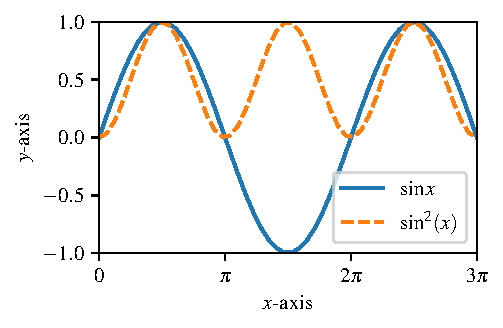
\includegraphics[scale=.65]{./img/myplot}
	% If not, use
	%\picplace{5cm}{2cm} % Give the correct figure height and width in cm
	\caption{\label{fig:matlpotlib} A plot created with PythonTeX}
\end{figure}
%En este capítulo introducimos algunos conceptos básicos concernientes al cálculo en una escala de tiempo. Una \emph{escala de tiempo} es un subconjunto arbitrario no vacío de los números reales. Así, \[ \mathds{R},\quad\mathds{Z},\quad\mathds{N},\quad\mathds{N}_{0}, \] es decir, los números reales, los enteros, los números naturales, y los enteros no negativos son ejemplos de escala de tiempo, como son \[ \left[0,1\right]\cup\left[2,3\right],\quad\left[0,1\right]\cup\mathds{N},\quad\text{el conjunto de Cantor}, \] mientras que \[ \mathds{Q},\quad\mathds{R}\setminus\mathds{Q},\quad\mathds{C},\quad\left(0,1\right), \] los números racionales, los números irracionales, los números complejos y el intervalo abierto entro $0$ y $1$, \emph{no} son escalas de tiempo. A lo largo de esta monografía denotaremos una escala de tiempo por el símbolo $\mathds{T}$. Asumiremos que una escala de tiempo $\mathds{T}$ tiene la topología que hereda de los números reales con la topología estándar.

El cálculo de escala de tiempo fue iniciado por Stefan Hilger, a fin de crear una teoría que pueda unificar el análisis discreto y continuo. En efecto, abajo en la sección 1.2 introduciremos la derivada delta $f^{\Delta}$ para una función $f$ definida sobre $\mathds{T}$, y resulta que
\begin{enumerate}
	\item $f^{\Delta}=f^{\prime}$ es la derivada usual si $\mathds{T}=\mathds{R}$ y
	\item $f^{\Delta}=\Delta f$ es el operador diferencia posterior usual si $\mathds{T}=\mathds{Z}$.
\end{enumerate}
En esta sección introducimos las nociones básicas conectadas a las escalas de tiempo. Empezamos definiendo los operadores salto posterior y anterior.

\section{Introducción}

\begin{definition}[Escala de tiempo]
Sea $\mathds{T}$ una escala de tiempo. Para $t\in\mathds{T}$ definimos el \emph{operador salto posterior} $\sigma\colon\mathds{T}\rightarrow\mathds{T}$ por \[ \sigma(t)\coloneqq\inf\left\{s\in\mathds{T}:s>t\right\}\quad\text{ para cualquier }\quad t\in\mathds{T}, \] mientras que el \emph{operador salto anterior} $\rho\colon\mathds{T}\rightarrow\mathds{T}$ es definido por \[ \rho(t)\coloneqq\sup\left\{s\in\mathds{T}:s<t\right\}\quad\text{ para cualquier }\quad t\in\mathds{T}. \] En esta definición agregamos el $\inf\emptyset=\sup\mathds{T}$, es decir, $\sigma(M)=M$ si $T$ tiene un máximo $M$ y el $\sup\emptyset=\inf\mathds{T}$, es decir, $\rho(m)=m$ si $\mathds{T}$ tiene un mínimo $m$. Si $\sigma(t)>t$, diremos que $t$ es \emph{dispersa a la derecha}, mientras que si $\rho(t)<t$ diremos que $t$ es \emph{dispersa a la izquierda}. Puntos que son dispersos a la derecha y dispersos a la izquierda en el mismo tiempo son llamados \emph{aislados}. También, si $t<\sup\mathds{T}$ y $\sigma(t)=t$, entonces $t$ es llamado \emph{denso a la derecha}, y si $t>\inf\mathds{T}$ y $\rho=t$, entonces $t$ es llamado \emph{denso a la izquierda}. Los puntos que son denso derecha y denso izquierda se llaman \emph{densos}. Si $T$ tiene un máximo disperso a la derecha $M$, entonces definimos $\mathds{T}^{\kappa}=\mathds{T}\setminus\{M\}$, caso contrario $\mathds{T}^{\kappa}=\mathds{T}$. Finalmente, la función \emph{grano} $\mu\colon\mathds{T}\rightarrow\left[0,\infty\right)$ es definida por \[ \mu(t)\coloneqq\sigma(t)-t\quad\text{para cualquier}\quad t\in\mathds{T}. \]
\end{definition}

\section{Diferenciación}

Ahora consideremos una función $f\colon\mathds{T}\rightarrow\mathds{R}$ y definir el llamado delta derivada (o Hilger) de $f$ en un punto $t\in\mathds{T}^{\kappa}$.

\begin{definition}[Delta diferenciable]
	Asuma que $f\colon\mathds{T}\rightarrow\mathds{R}$ es una función y sea $t\in\mathds{T}^{\kappa}$. Entonces definimos el número $f^{\Delta}(t)$  (siempre que este exista) con la propiedad que dado cualquier $\varepsilon>0$, existe una vecindad $U$ de $t$ (es decir, $U=\left(t-\delta\right)\cap\mathds{T}$ para algún $\delta>0$) tal que \[ |f(\sigma(t))|-f(s)-f^{\Delta}(t)(\sigma(t)-s)|\leq\varepsilon|\sigma(t)-s|\quad\text{para cualquier}\quad s\in U. \] Llamamos $f^{\Delta}(t)$ la derivada delta (o Hilger) de $f$ en $t$. Es más, diremos que $f$ es \emph{delta} (o Hilger) \emph{diferenciable} (o en breve: \emph{diferenciable}) en $\mathds{T}^{\kappa}$ siempre que $f^{\Delta}(t)$ exista para cualquier $t\in\mathds{T}^{\kappa}$. La función $f^{\Delta}\colon\mathds{T}^{\kappa}\rightarrow\mathds{R}$ es entonces llamada la derivada (delta) de $f$ sobre $\mathds{T}^{\kappa}$.

	Algunas relaciones sencillas y útiles en relación con la derivada delta se dan a continuación.
\end{definition}

\begin{theorem}{}
	Asuma que $f\colon\mathds{T}\rightarrow\mathds{R}$ es una función y sea $t\in\mathds{T}^{k}$. Entonces tenemos lo siguiente:
	\begin{enumerate}
		\item Si $f$ es diferenciable en $\mathds{T}$, entonces $f$ es continua en $t$.
		\item Si $f$ es continua en $t$ y $t$ es dispersa a la derecha, entonces $f$ es diferenciable en $t$ con \[ f^{\Delta}(t)=\frac{f(\sigma(t))-f(t)}{\mu(t)}. \]
		\item Si $t$ es densa a la derecha, entonces $f$ es diferenciable en $t$ sii el límite \[ \lim_{s\to t}\frac{f(t)-f(s)}{t-s} \] existe como un número finito. En este caso \[ f^{\Delta}(t)=\lim_{s\to t}\frac{f(t)-f(s)}{t-s}. \]
		\item Si $f$ es diferenciable en $t$, entonces \[ f(\sigma(t))=f(t)+\mu(t)f^{\Delta}(t). \]
	\end{enumerate}
\end{theorem}
\begin{exercise}
	Muestre que si $\mathds{T}=q^{\mathds{N}_{0}}\coloneqq\left\{q^{n}:n\in\mathds{N}_{0}\right\}$, $q>1$, entonces \[ {\left(\log t\right)}^{\Delta}=\frac{\log q}{q-1}\cdot\frac{1}{t}. \]
\end{exercise}
\begin{example}{}
	Nuevamente consideremos los dos casos $\mathds{T}=\mathds{R}$ y $\mathds{T}=\mathds{Z}$.
	\begin{enumerate}
		\item Si $\mathds{T}=\mathds{R}$, entonces el Teorema 1.3 resulta que $f\colon\mathds{R}\rightarrow\mathds{R}$ es delta diferenciable en $t\in\mathds{R}$ sii \[ f^{\prime}(t)=\lim_{s\to t}\frac{f(t)-f(s)}{t-s}\quad\text{existe}, \] es decir, sii $f$ es diferenciable (en el sentido clásico) en $t$. En este caso tenemos entonces \[ f^{\Delta}(t)=\lim_{s\to t}\frac{f(t)-f(s)}{t-s}=f^{\prime}(t) \] por el Teorema 1.3 (iii).
		\item Si $\mathds{T}=\mathds{Z}$, entonces el Teorema 1.3 (ii) resulta que $f\colon\mathds{Z}\rightarrow\mathds{R}$ es delta diferenciable en $t\in\mathds{Z}$ con \[ f^{\Delta}(t)=\frac{f(\sigma(t))-f(t)}{\mu(t)}=\frac{f(t+1)-f(t)}{1}=f(t+1)-f(t)=\Delta f(t), \] donde $\Delta$ es el \emph{operador diferencia posterior} usual definida por la última ecuación de arriba.
	\end{enumerate}
\end{example}

A continuación, nos gustaría poder encontrar las derivadas de sumas, productos, y cocientes de funciones diferenciables. Esto es posible de acuerdo con el siguiente teorema:
\begin{theorem}{}
	Asuma que $f,g\colon\mathds{T}\rightarrow\mathds{R}$ son diferenciables en $t\in\mathds{T}^{\kappa}$. Entonces
	\begin{enumerate}
		\item La suma de $f+g\colon\mathds{T}\rightarrow\mathds{R}$ es diferenciable en $a$ con \[ {\left(f+g\right)}^{\Delta}(t)=f^{\Delta}(t)+g^{\Delta}(t). \]
		\item Para cualquier constante $\alpha$, $\alpha f\colon\mathds{T}\rightarrow\mathds{R}$ es diferenciable en $t$ con \[ {\left(\alpha f\right)}^{\Delta}\left(t\right)=f^{\Delta}\left(t\right)+g^{\Delta}\left(t\right). \]
		\item El producto $fg\colon\mathds{T}\rightarrow\mathds{R}$ es diferenciable en $t$ con \[ {\left(fg\right)}^{\Delta}\left(t\right)=f^{\Delta}\left(t\right)g\left(t\right)+f\left(\sigma\left(t\right)\right)g^{\Delta}\left(t\right)=f\left(t\right)g^{\Delta}\left(t\right)+f^{\Delta}\left(t\right)g\left(\sigma\left(t\right)\right). \]
		\item Si $f\left(t\right)f\left(\sigma\left(t\right)\right)\neq0$, entonces $\frac{1}{f}$ es diferenciable en $t$ con \[ {\left(\frac{1}{f}\right)}^{\Delta}\left(t\right)=-\frac{f^{\Delta}\left(t\right)}{f\left(t\right)f\left(\sigma\left(t\right)\right)}. \]
		\item Si $g\left(t\right)g\left(\sigma\left(t\right)\right)\neq0$, entonces $\frac{f}{g}$ es diferenciable en $t$ y \[ {\left(\frac{f}{g}\right)}^{\Delta}\left(t\right)=\frac{f^{\Delta}\left(t\right)g\left(t\right)-f\left(t\right)g^{\Delta}\left(t\right)}{g\left(t\right)g\left(\sigma\left(t\right)\right)}. \]
	\end{enumerate}
\end{theorem}
\begin{proof}
	Asuma que $f$ y $g$ son delta diferenciables en $t\in\mathds{T}^{\kappa}$.
	\begin{enumerate}
		\item Sea $\varepsilon>0$. Entonces, existen vecindades $U_{1}$ y $U_{2}$ de $t$ con \[ \left|f\left(\sigma\left(t\right)\right)-f\left(s\right)-f^{\Delta}\left(t\right)\left(\sigma\left(t\right)-s\right)\right|\leq\frac{\varepsilon}{2}\left|\sigma\left(t\right)-s\right|\quad\text{para todo}\quad s\in U_{1} \] y \[ \left|g\left(\sigma\left(t\right)\right)-g\left(s\right)-g^{\Delta}\left(t\right)\left(\sigma\left(t\right)-s\right)\right|\leq\frac{\varepsilon}{2}\left|\sigma\left(t\right)-s\right|\quad\text{para todo}\quad s\in U_{2}. \] Sea $U=U_{1}\cap U_{2}$. Entonces tenemos para todo $s\in U$
		\begin{align*}
		=+\\
		\end{align*}
		Por lo tanto, $f+g$ es diferenciable en $t$ y ${\left(\right)}^{\Delta}$
	\end{enumerate}
\end{proof}
%%\sectionmark{Ejercicios}
\section*{Ejercicios}
\begin{prob}{Sucesión contractiva}
	Una sucesión $\left\{x_{n}\right\}$ se dice que \textbf{contractiva} si $\exists$ alguna constante $c$, $0<c<1\ni\forall\,n\in\mathds{N}$, $|x_{n+2}-x_{n+1}|\leq c|x_{n+1}-x_{n}|$. Pruebe que una sucesión contractiva debe ser una sucesión de Cauchy, y por lo tanto converge.
\end{prob}

\begin{prob}{Media aritmética recursiva}
Sea $a\neq b$ números reales arbitrarios, y defina la sucesión $\left\{x_{n}\right\}$ por \[ x_{1}=a,x_{2}=b,\text{ y }\forall\,n\in\mathds{N},x_{n+2}=\frac{x_{n+1}+x_{n}}{2}. \] Esto es, cada nuevo término está iniciando con el tercero que es el promedio de los dos términos previos.
	\begin{enumerate}
		\item Pruebe que $\left\{x_{n}\right\}$ converge probando que este es una sucesión constructiva.
		\item Pruebe que $\forall\,n\in\mathds{N}$, $x_{n+1}+\frac{1}{2}x_{n}=b+\frac{1}{2}a$.\label{9b}
		\item Use~\ref{9b} y el álgebra de límites para encontrar que  $\lim\limits_{n\to\infty}x_{n}$. ?`Está sorprendido por la respuesta? Note que si usted intercambia $a$ y $b$ la respuesta podría ser diferente.
	\end{enumerate}
\end{prob}

\begin{prob}{Media aritmética ponderada recursiva}
	Sean $a\neq b$ dos números reales arbitrarios, sea $0<t<1$, y defina la sucesión $\left\{x_{n}\right\}$ por \[ x_{1}=a,x_{2}=b,\text{ z }\forall\,n\in\mathds{N},x_{n+2}=tx_{n}+\left(1-t\right)x_{n+1}. \] Esto es, cada nuevo término que inicia con el tercero que es el promedio ponderado de los términos previos. Geométricamente, $x_{n+2}$ es un punto en el intervalo entre $x_{n}$ y $x_{n+1}$ que corta el intervalo en dos segmentos cuyas longitudes están en la proporción $t$ a $1-t$. Pruebe que $\left\{x_{n}\right\}$ es contractiva, y encuentre su límite.
\end{prob}

\begin{prob}{Aplicación contractiva}
	Sean $a<b$ e $I=\left[a,b\right]$. Una función $f\colon I\rightarrow I$ se dice que es una \textbf{contracción} si $\exists c\ni0<c<1$ y $\forall\,x,y\in I$, $|f\left(x\right)-f\left(y\right)|\leq c|x-y|$. Pruebe que una aplicación contractiva debe tener por lo menos un ``punto fijo'', $x\in I\ni f\left(x\right)=x$. También pruebe que $f$ no puede tener más de un punto fijo en $I$.
\end{prob}

\begin{prob}{Números de Fibonacci}
	La sucesión de Fibonacci consiste de los números de Fibonacci, $1,1,2,3,5,8,13,21,\ldots$, y está definido recursivamente por $f_{1}=1$, $f_{2}=1$, y $\forall\,n\geq2$, $f_{n+2}=f_{n+1}+f_{n}$. Cada nuevo término después del segundo es la suma de los dos términos previos. Muchos resultados interesantes han sido probados acerca de los números de Fibonacci--lo suficiente para llenar un libro entero. Deberemos concentrarnos aquí con la sucesión de proporciones de los sucesivos números de Fibonacci. Empezamos definiendo la sucesión por $r_{n}=\tfrac{f_{n+1}}{f_{n}}$.
		\begin{enumerate}
			\item Desarrolle una tabla que muestre los primeros diez términos de $\left\{r_{n}\right\}$. En la basa de esta tabla, conjeture las respuestas a las siguientes preguntas. ?`$\left\{r_{n}\right\}$ es convergente? ?`Es monótona? ?`Eventualmente monótona? ?`Puede encontrar una subsucesión estrictamente creciente? ?`Una subsucesión estrictamente decreciente? (No se requieren demostraciones).
			\item Pruebe que $\forall\,n\in\mathds{N}$, $r_{n+1}=1+\tfrac{1}{r_{n}}$.
			\item Pruebe que $\forall\,n\geq2$, $\tfrac{3}{2}<r_{n}<2$.
			\item Pruebe que $\left\{r_{n}\right\}$ es ``contractiva'', y por lo tanto es una sucesión de Cauchy.
			\item Encuentre $\lim\limits_{n\to\infty}r_{n}$. [Tome nota de este límite; este reaparecerá.]
			\item La ecuación cuadrática $x^{2}-x-1=0$ tiene dos soluciones, $\alpha=\frac{1+\sqrt{5}}{2}$ y $\beta=\frac{1-\sqrt{5}}{2}$. Muestre que $\alpha+\beta=1$, $\alpha^{2}=a+1$, y $\beta^{2}=\beta+1$, y desde estos hechos muestre que $\forall\,n\in\mathbb{N}$, $\alpha^{n+2}=\alpha^{n+1}+\alpha^{n}$ y $\beta^{n+2}=\beta^{n+1}+\beta^{n}$.\label{9f}
			\item $\forall\,n\in\mathds{N}$, defina $u_{n}=\frac{\alpha^{n}-\beta^{n}}{\alpha-\beta}$, donde $\alpha$ y $\beta$ están definidos en~\ref{9f}. Pruebe que $u_{1}=1$, $u_{2}=1$, y $\forall\,n\geq2$, $u_{n+2}=u_{n+1}+u_{n}$. Por lo tanto, $\left\{u_{n}\right\}$ debe ser la sucesión de Fibonacci. Tenemos encontrado una fórmula para los números de Fibonacci: $f_{n}=u_{n}$.
			\item \textbf{Significado geométrico} de $\alpha$. Considere un rectángulo cuyo ancho $\alpha$ y largo $a+b$ son así proporcionados que cuando un cuadrado de lado $a$ es removido, como se muestra aquí, el rectángulo restante tiene ancho y longitud en la misma proporción. Esto es, $\tfrac{a+b}{a}=\tfrac{a}{b}$.
	
			Los matemáticos de la Grecia clásica llamaron esta proporción $R=\frac{a}{b}$ la ``\textbf{Proporción áurea}'' y cualquier rectángulo con lados en la proporción un ``\textbf{rectángulo áureo}''. Ellos consideraron esto como la más estéticamente agradable de todos los rectángulos, y se usó esto frecuentemente en su arte y arquitectura. Pruebe algebraicamente que $R=\alpha$, definida en~\ref{9f} arriba.
			\item Pruebe que $\forall\,n\geq2$, $\forall\,n\geq2$, $f_{n+1}f_{n-1}-{\left(f_{n}\right)}^{2}={\left(-1\right)}^{n}$.
			\item Pruebe que $\forall\,n\in\mathds{N}$, $r_{n+1}-r_{n}=\frac{{\left(-1\right)}^{n+1}}{f_{n}f_{n+1}}$.\label{9j}
			\item Use~\ref{9j} para probar que $\left\{r_{2n}\right\}$ es estrictamente decreciente y $\left\{r_{2n+1}\right\}$ es estrictamente creciente.
	\end{enumerate}
\end{prob}

\begin{prob}{}
	Sea $a\geq1$. Defina la sucesión $\left\{x_{n}\right\}$ por $x_{1}=a$, y $x_{n+1}=a+\frac{1}{x_{m}}$. Pruebe que $\forall\,n\geq2$, $a+\frac{1}{2a}\leq x_{n}\leq 2a$, y use este resultado para probar que $x_{n}$ es contractiva. Encuentre $\lim\limits_{n\to\infty}x_{n}$.
\end{prob}

\begin{prob}{}
	Sea $a>1$. Defina la sucesión $\left\{x_{n}\right\}$ por $x_{1}=a$ y $x_{n}=\frac{1}{a+x_{n}}$. Pruebe que $\forall\,n\in\mathds{N}$, $\frac{1}{2a}\leq x_{n}\leq a$, y use este resultado para probar que $\left\{x_{n}\right\}$ es contractiva. Encuentre el $\lim\limits_{n\to\infty}x_{n}$. Compare este límite con el ejercicio anterior.
\end{prob}
\endgroup
\renewcommand{\refname}{Referencias bibliográficas}
\nocite{*}
\bibliographystyle{spmpsci}
{\footnotesize 
	\bibliography{bib}}
%[title={Referencias bibliográficas},heading=bibintoc]}
%\biblstarthook{In view of the parallel print and (chapter-wise) online publication of your book at \url{www.springerlink.com} it has been decided that -- as a genreral rule --  references should be sorted chapter-wise and placed at the end of the individual chapters. However, upon agreement with your contact at Springer you may list your references in a single seperate chapter at the end of your book. Deactivate the class option \texttt{sectrefs} and the \texttt{thebibliography} environment will be put out as a chapter of its own.\\\indent
%References may be \textit{cited} in the text either by number (preferred) or by author/year.\footnote{Make sure that all references from the list are cited in the text. Those not cited should be moved to a separate \textit{Further Reading} section or chapter.} If the citatiion in the text is numbered, the reference list should be arranged in ascending order. If the citation in the text is author/year, the reference list should be \textit{sorted} alphabetically and if there are several works by the same author, the following order should be used:
%%%%%%%%%%%%%%%%%%%%%%%%%%%%%%%%%%%%%%%%%%%%%%%%%%%%%%%%%%%%%%%%%%%%%%%%%%%%%%%%%%%%%%%%%%%%%%%
\backmatter
%\appendix
\motto{All's well that ends well}
%\chapter{Chapter Heading}
%\label{introA} % Always give a unique label
% use \chaptermark{}
% to alter or adjust the chapter heading in the running head

\section{Section Heading}
\label{sec:A1}
% Always give a unique label
% and use \ref{<label>} for cross-references
% and \cite{<label>} for bibliographic references
% use \sectionmark{}
% to alter or adjust the section heading in the running head
Instead of simply listing headings of different levels we recommend to let every heading be followed by at least a short passage of text. Furtheron please use the \LaTeX\ automatism for all your cross-references and citations.

\subsection{Subsection Heading}
\label{sec:A2}
Instead of simply listing headings of different levels we recommend to let every heading be followed by at least a short passage of text. Furtheron please use the \LaTeX\ automatism for all your cross-references and citations as has already been described in Sect.~\ref{sec:A1}.

For multiline equations we recommend to use the \verb|eqnarray| environment.
\begin{eqnarray}
\vec{a}\times\vec{b}=\vec{c} \nonumber\\
\vec{a}\times\vec{b}=\vec{c}
\label{eq:A01}
\end{eqnarray}

\subsubsection{Subsubsection Heading}
Instead of simply listing headings of different levels we recommend to let every heading be followed by at least a short passage of text. Furtheron please use the \LaTeX\ automatism for all your cross-references and citations as has already been described in Sect.~\ref{sec:A2}.

Please note that the first line of text that follows a heading is not indented, whereas the first lines of all subsequent paragraphs are.

% For figures use
%
\begin{figure}[t]
\sidecaption[t]
%\centering
% Use the relevant command for your figure-insertion program
% to insert the figure file.
% For example, with the option graphics use
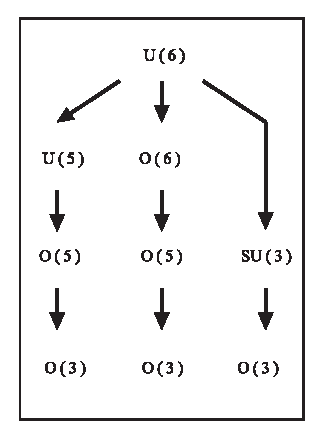
\includegraphics[scale=.65]{figure}
%
% If not, use
%\picplace{5cm}{2cm} % Give the correct figure height and width in cm
%
\caption{Please write your figure caption here}
\label{fig:A1}       % Give a unique label
\end{figure}

% For tables use
%
\begin{table}
\caption{Please write your table caption here}
\label{tab:A1}       % Give a unique label
%
% For LaTeX tables use
%
\begin{tabular}{p{2cm}p{2.4cm}p{2cm}p{4.9cm}}
\hline\noalign{\smallskip}
Classes & Subclass & Length & Action Mechanism  \\
\noalign{\smallskip}\hline\noalign{\smallskip}
Translation & mRNA$^a$  & 22 (19--25) & Translation repression, mRNA cleavage\\
Translation & mRNA cleavage & 21 & mRNA cleavage\\
Translation & mRNA  & 21--22 & mRNA cleavage\\
Translation & mRNA  & 24--26 & Histone and DNA Modification\\
\noalign{\smallskip}\hline\noalign{\smallskip}
\end{tabular}
$^a$ Table foot note (with superscript)
\end{table}
%\Extrachap{Glosario}

\runinhead{término del glosario}
%
\Extrachap{Soluciones}

\section*{Problemas del Capítulo~\ref{intro}}

\begin{sol}{prob1}
The solution\index{problems}\index{solutions} is revealed here.
\end{sol}


\begin{sol}{prob2}
\textbf{Problem Heading}\\
(a) The solution of first part is revealed here.\\
(b) The solution of second part is revealed here.
\end{sol}


\printindex
\end{document}